\documentclass[12pt,letterpaper,oneside]{report}
%\input macros.tex
%\includeonly{seccion_0,seccion_resumen, seccion_1, referencias, anexos}

% ==========================================
% PAQUETES NECESARIOS
% ==========================================
\usepackage[utf8]{inputenc}
\usepackage[spanish,es-tabla]{babel}
\usepackage{graphicx}
\usepackage{array}
\usepackage{amsmath, amssymb}
\usepackage{geometry}
\geometry{letterpaper, left=3cm, right=3cm, top=3cm, bottom=3cm}
\usepackage{subcaption}
\usepackage{setspace}
\usepackage{acronym}
\usepackage{hyperref}
\hypersetup{
    hidelinks
}
\usepackage{xcolor} % Para los colores
\usepackage{titlesec} % Para personalizar los títulos
\usepackage{tikz}
\usetikzlibrary{arrows.meta, positioning}

% ==========================================
% CONFIGURACIÓN DEL FORMATO DE CAPÍTULOS
% ==========================================
\definecolor{verde_antioquia}{RGB}{0, 155, 77} % Puedes ajustar el color aquí
\definecolor{gris_numero}{HTML}{D3D3D3} % Un gris claro o el azul de tu imagen
\definecolor{verdeUdeA}{rgb}{0.325,0.506,0.208} %rgb=83,129,53


\titleformat{\chapter}[display]
  {\normalfont\bfseries\raggedleft} % Alineación a la derecha
  {\color{verde_antioquia}\fontsize{100}{100}\selectfont\thechapter} % Número gigante
  {-20pt} % Espacio entre el número y el título
  {\Huge} % Tamaño del nombre del capítulo (más grande que el texto)
  [\vspace{1cm}]

% Para que los capítulos sin número (Agradecimientos, etc.) también estén a la derecha
\titleformat{name=\chapter,numberless}[display]
  {\normalfont\bfseries\raggedleft}
  {}
  {-40pt}
  {\Huge}
  [\vspace{1cm}]

% ==========================================
% INICIO DEL DOCUMENTO
% ==========================================



\begin{document}

% ==========================================
% PORTADA (Página 1)
% ==========================================
\begin{titlepage}
    \centering
    %\vspace*{0.5cm}
        \vfill
    
\includegraphics[width=0.35\textwidth]{escudo_udea.png}\\[1cm]
    
    {\Large \textbf{Estudio del crecimiento de cristales de hemozoína ($\beta$-hematina) en \textit{Plasmodium falciparum} mediante un modelo de Monte Carlo cinético }}\\[1.5cm]
    
    {\Large \textbf{Sebastian Gaviria Giraldo}}\\[1.5cm]
    
    {\large Tesis para optar al título de Físico}\\[1.5cm]

    {\large \textbf{Asesores}}\\[0.5cm]
    {\large Olga Lucía López Acevedo, Ph.D. en Física Teórica}\\
    {\large Hernán David Salinas Jiménez, Ph.D. en Física}\\[1.5cm]
    

    {\large Universidad de Antioquia}\\[0.2cm]
    {\large Facultad de ciencias exactas y naturales}\\[0.2cm]
    {\large Instituto de Física}\\[0.2cm]
    {\large Medellín}\\[0.8cm]
    {\large Agosto, 2026}
\end{titlepage}

\newpage

    
    \begin{center}
    %\vspace*{0.5cm}
        \vfill
    
\includegraphics[width=0.35\textwidth]{escudo_udea.png}
    \end{center}

\begin{center}

    %--------------------------------------------------
    
    \thispagestyle{empty}
    %{\arrayrulecolor{verdeUdeA}
    \footnotesize{\begin{tabular}{cm{10cm}} 
    \noalign{\color{verdeUdeA}\hrule height 3pt}
    \textbf{Cita} & \hspace{2cm} (Gaviria Giraldo, 2026) \\ \hline
    %
    \parbox[c][2.0\height]{5cm}{\centerline{\textbf{Referencia}} 
        }
     & \hspace{-0.15cm} Gaviria Giraldo, S. (2026). Estudio del crecimiento de cristales de hemozoína ($\beta$-hematina) en \textit{Plasmodium falciparum} mediante un modelo de Monte Carlo cinético. \\ 

     \\

     \parbox[c][2.0\height]{5cm}{\centerline{\textbf{Estilo APA 7 (2020)}} 
        }
     & \hspace{-0.15cm} Trabajo de grado profesional. Universidad de Antioquia, Medellín, Colombia. \\
    \noalign{\color{verdeUdeA}\hrule height 3pt}
\end{tabular}}

%\arrayrulecolor{black}

\end{center}



\noindent \vspace{-0.5cm}
\includegraphics{CC.jpg}\quad

\includegraphics{CCima.png}

\vspace{1cm}
%
\noindent 
\includegraphics[scale=0.35]{escudo_udea_vice.png}\quad

\includegraphics{sis_biblo.png}\\
%
Biblioteca Carlos Gaviria Diaz\\[1cm]
%
\textbf{Repositorio Institucional:} http://bibliotecadigital.udea.edu.co\\[1cm]

\noindent Universidad de Antioquia - www.udea.edu.co\\[0.5cm]
%\textbf{Rector:} Nombres y Apellidos.\\
%\textbf{Decano/Director} Nombres y Apellidos.\\
%\textbf{Jefe departamento:} Nombres y Apellidos.\\[1cm]

\noindent El contenido de esta obra corresponde al derecho de expresión de los autores y no compromete el pensamiento institucional de la Universidad de Antioquia ni desata su responsabilidad frente a terceros. Los autores asumen la responsabilidad por los derechos de autor y conexos.

%--------------------reemplase hasta aqui------------------




% ==========================================
% DERECHOS DE AUTOR (Página 2)
% ==========================================
%\newpage
%\thispagestyle{empty}
%\vspace*{\fill}
%\begin{center}
%    Sebastian Gaviria Giraldo\\
%    all rights reserved, 2026
%\end{center}
%\vspace*{\fill}
\newpage

% Comenzar numeración arábiga en la página 3
\pagenumbering{arabic}
\setcounter{page}{3}

% ==========================================
% AGRADECIMIENTOS (Página 3)
% ==========================================
\chapter*{Agradecimientos}
\addcontentsline{toc}{chapter}{Agradecimientos}

Primero que todo, quiero agradecer a mi familia, amigos y compañeros, por habitar conmigo este pequeño pedazo de espacio-tiempo. Especialmente, agradezco a mi madre Teresa, por todas las madrugadas que se pegó para que yo tuviera algo qué comer durante el día. Agradezco su apoyo emocional y su comprensión única hacia mí. Agradezco su cariño y sus regaños, que siempre han sido en pro de mi bienestar. Le agradezco por ser la mano que más fuerte agarró la mía en los momentos que más lo necesité, y le agradezco infinitamente por haberme salvado, con su ternura y amor, de un destino que no era el mío. También agradezco a mi hermana Jhoana por ser ese ejemplo de superación y tenacidad, por ser un referente en la vida y en lo profesional. Aunque siempre estaré agradecido con toda mi familia, ellas dos son mi fortaleza y la principal motivación detrás de todas mis luchas, alegrías y sueños. Quiero agradecer también a la profe Olga y al profe Hernan por su acompañamiento durante este proceso de trabajo de grado. Su paciencia, consejos y constante disposición siempre que los necesité fueron fundamentales para culminar satisfactoriamente este proyecto. Son para mí, además de dos grandes profesionales en lo que hacen, dos grandes personas, admirables en todos los aspectos. También quiero agradecer a Daniel Duque que, dentro del marco de su trabajo como joven investigador, fue un apoyo fundamental, especialmente en lo concerniente a los cálculos de potenciales interatómicos y el uso de MACE. También agradecer al proyecto Programática 2024-76972 que hizo posible la ejecución del trabajo y la disposición de datos experimentales y al estudiante de maestría Germán Torres, por la base inicial del código implementado. Finalmente, le agradezco a todos los compañeros con los que pude compartir un rato durante mi proceso formativo en la Universidad de Antioquia, ya que a partir de las charlas, las discusiones, y los parches que propiciamos pude aprender de cada uno de ellos.

\newpage
% ==========================================
% DEDICATORIA (Página 4)
% ==========================================
\chapter*{Dedicatoria}
\addcontentsline{toc}{chapter}{Dedicatoria}
\vspace*{3cm}
\begin{flushright}
    \textit{Para mi abuela Blanca, para Billy y Dakota. Aunque ahora no están presentes materialmente, siempre lo estarán en mis pensamientos y en cada paso que doy...}
\end{flushright}

\newpage
% ==========================================
% RESUMEN (Página 5)
% ==========================================
\chapter*{Resumen}
\addcontentsline{toc}{chapter}{Resumen}

En este trabajo se desarrolló un modelo de Monte Carlo cinético (kMC) para describir el crecimiento cristalino de la hemozoína, o su análogo sintético $\beta$-hematina, como parte del proceso de detoxificación del hemo en \textit{Plasmodium falciparum}.  El trabajo revisa las rutas de cristalización desde un enfoque   clásico representando la formación de hemozoína mediante eventos de adsorción, desorción, difusión superficial (migración) e incorporación sobre sitios con distinta coordinación. Con base en este marco, se implementó un esquema de kMC apoyado en el algoritmo BKL, capaz de traducir las tasas de transición en evolución temporal física. La implementación fue validada mediante la reproducción de resultados reportados en la literatura para el crecimiento cristalino de lisozima en la que se evidencian los diferentes regímenes de crecimiento dependiendo de la sobresaturación. Posteriormente se aplicó al estudio del crecimiento de hemozoína en redes 2D y 3D, considerando configuraciones isotrópicas y anisotrópicas. De manera complementaria, se realizaron cálculos con potenciales interatómicos basados en aprendizaje automático, particularmente MACE, con el propósito de explorar la estimación de parámetros energéticos asociados a los eventos incluidos en el modelo. Los resultados muestran trayectorias de porcentaje de conversión y morfologías superficiales que evidencian una dependencia del régimen de crecimiento con la configuración de la red y con los parámetros cinéticos escogidos.

%A partir de las herramientas multidisciplinares que entrega la física, y en este caso la física estadística, se buscó construir un modelo de Monte Carlo cinético (kMC) que permitiera entender con mayor profundidad física los mecanismos microscópicos del crecimiento de cristales de hemozoína (o su análogo sintético, $\beta$ - hematina). A partir de primeros principios, con la ayuda de simulaciones basadas en DFT y el modelo MACE (ASE), se lograron calibrar los parámetros del modelo kMC que reproducen con fiabilidad físico-química el comportamiento de los mecanismos de cristalización de las diferentes caras de la hemozoína. A raíz de varios experimentos computacionales diferentes, se logró reproducir el porcentaje de conversión, la rugosidad, entre otros observables macroscópicos presentes en la literatura y en los estudios especializados en el tema. 

\newpage
% ==========================================
% ÍNDICES (Páginas 6 - 8)
% ==========================================
\tableofcontents % Índice general

\newpage
\listoffigures % Índice de figuras
\addcontentsline{toc}{chapter}{Índice de figuras}

\newpage
% ==========================================
% LISTA DE ABREVIACIONES (Página 9)
% ==========================================
\chapter*{Lista de abreviaciones}
\addcontentsline{toc}{chapter}{Lista de abreviaciones}
\begin{acronym}[MTD] % MTD es la palabra más larga para alinear
    \acro{HZ}{Hemozoína}
    \acro{BH}{$\beta$-hematina}
    \acro{VD}{Vacuola Digestiva}
    \acro{kMC}{Monte Carlo cinético}
    \acro{UC}{Unidad de Crecimiento}
    \acro{CNT}{Teoría Clásica de Nucleación}
    \acro{DFT}{Teoría del funcional de la densidad}
\end{acronym}

\newpage
% ==========================================
% CAPÍTULOS DE LA TESIS
% ==========================================

\chapter{Introducción}



La condición transversal de los métodos, técnicas e ideas desarrolladas por la física ha permitido abordar múltiples tipos de problemas desde los distintos enfoques que esta ciencia ofrece. Uno de los rasgos más valiosos que se adquieren a lo largo de la formación como físico es la capacidad de integración multidisciplinaria, que permite reconocer estructuras conceptuales comunes en fenómenos aparentemente muy distintos. Bajo esta perspectiva, no es raro que el problema de la malaria, tan aparentemente alejado de las ciencias físicas, pueda ser estudiado cuando se enfoca desde los principios apropiados. En particular, al observar el ciclo de vida del parásito de la malaria, podemos identificar que se presentan algunos procesos físicoquímicos interesantes que vale la pena explorar. Concretamente, en los procesos concernientes a la digestión de la hemoglobina dentro de su vacuola digestiva (VD), ocurren algunos procesos de cristalización, que permiten al parásito seguir con vida y proliferar dentro del huesped infectado \cite{Kapishnikov2011}. Por esta razón, comprender con mayor detalle mecanicista estos procesos de cristalización se ha convertido en uno de los principales blancos farmacológicos para atacar el parásito de la malaria y combatir la enfermedad.\\

Desde este punto de vista, la física puede aportar herramientas conceptuales y metodológicas valiosas para la comprensión de dichos mecanismos. Es bien sabido, desde la termodinámica y la físicoquímica, que durante los procesos de crecimiento cristalino ocurren algunos eventos dinámicos, como los conocidos procesos de adsorción, desorción y difusión superficial (migración), los cuales determinan la evolución temporal y morfológica del sistema. Si además se consideran las escalas temporales y espaciales adecuadas, estos mismos eventos pueden ser tratados de forma aproximada con modelos estocásticos, dando entrada así a la física estadística y a la física computacional como herramientas particularmente útiles para estudiar este tipo de problemas. De esta manera, el estudio de la cristalización de Hemozoína (HZ) asociada a la malaria no solo se convierte en un problema de interés biológico y químico, sino también en un escenario ideal para aplicar modelos físicos que permitan capturar la complejidad del proceso desde una perspectiva microscópica, mesoscópica y probabilística. Dentro de los esfuerzos más recientes por abordar el estudio de la problemática de la malaria desde una perspectiva física, destaca la tesis de maestría de Cristian Alirio Parra, la cual constituye un antecedente importante para el presente estudio \cite{AlirioParra2023}. \\

Por otro lado, durante las últimas decadas, uno de los principales modelos estocásticos que ha tomado mayor relevancia para simular la dinámica de crecimiento de cristales es el conocido Monte Carlo  cinético (kMC por sus siglas en inglés). Este enfoque permite introducir escalas temporales reales en los pasos de simulación, proporcionando así una representación más fiel de la evolución dinámica del sistema. Además, en el corazón del kMC se tiene una lista de procesos elementales que pueden asociarse directamente con los eventos que participan en la nucleación y crecimiento de cristales. Las probabilidades relativas de tales eventos dependen de barreras de energía y de propiedades termodinámicas que, a su vez, pueden incorporarse de manera indirecta al modelo mediante cálculos más detallados, apoyados en el uso de la Teoría del Funcional de Densidad (DFT) y la Dinámica Molecular (MD). En este sentido, el kMC se presenta como una estrategia particularmente adecuada para conectar la descripción microscópica del sistema con su comportamiento mesoscópico y temporal, permitiendo así estudiar con mayor precisión los mecanismos que sostienen la formación de cristales relevantes en el contexto de la malaria. Por ejemplo, en los trabajos de Zhu et al. \cite{Zhu1992},
Schulze et al., \cite{Schulze2008} y Andersen et al. \cite{Andersen2019}, se pueden estudiar los fundamentos del kMC con ejemplos aplicados al crecimiento superficial de cristales. Mientras que Rak et al. \cite{Rak2001}, y Piana et al. \cite{Piana2006}, estudian estos mismos efectos teniendo en cuenta la interacción con solvente.  \\

% Agradecimientos también al Grupo programática (averiguar info más detallada con Hernan)

% Mencionar los resultados experimentales

% German Torres por la base de los códigos


\section{Hipótesis}
A partir de supuestos fisicoquímicos, y desde el marco teórico de la física estadística, se puede implementar un modelo de Monte Carlo cinético que reproduzca la cinética y morfología superficial del crecimiento de cristales de Hemozoína (o su análogo sintético $\beta$-hematina).\\

\section{Objetivos}
\subsection*{Objetivo General}
Diseñar, implementar y validar computacionalmente un modelo kMC, en versiones 2D y 3D, que reproduzca la cinética y morfología del crecimiento de cristales de hemozoína ($\beta$-hematina).\\

\subsection*{Objetivos específicos}
\begin{itemize}

    \item Identificar, a partir de la literatura, la unidad de crecimiento dimérica de la HZ (o su análogo sintético BH) para las simulaciones kMC.

    \item Comprender los diferentes tipos de enlace que conforman la estructura de los cristales de HZ.

    \item Estudiar las rutas clásicas de crecimiento de cristales de HZ.

    \item Definir tasas de transición de eventos elementales del modelo kMC que sean acordes con los mecanismos de cristalización de la HZ.

    \item Utilizar valores adecuados para los parámetros que controlan la cinética y morfología mesoscopica del crecimiento cristalino de HZ.

    \item Construir la implementación computacional del modelo y ejecutar diferentes simulaciones que permitan reconstruir acertadamente observables como el porcentaje de conversión y la morfología de crecimiento superficial.
    
\end{itemize}\\

\chapter{La problemática de la malaria}

La malaria es una enfermedad letal, pero tratable, común en regiones tropicales y subtropicales. Se transmite a los humanos por la picadura de mosquitos infectados del género \textit{Anopheles}, portadores de cualquiera de las especies de parásitos unicelulares del género \textit{Plasmodium} (\textit{Vivax}, \textit{Ovale}, \textit{Malariae}, \textit{Knowlesi} y \textit{Falciparum}). De acuerdo con el \textit{World malaria report 2025} de la Organización Mundial de la Salud, en 2024 se estimaron 282 millones de casos de malaria y 610\,000 muertes en 80 países endémicos, lo que representa un incremento con respecto a 2023, siendo el \textit{Plasmodium falciparum} el responsable de al menos el $50 \%$ de los casos reportados de Malaria en humanos, y esta cifra asciende a cerca del $95 \%$ cuando se trata de las muertes asociadas a la malaria. A pesar de ello, el informe también destaca avances importantes: desde el año 2000 se han evitado 2.3 mil millones de casos y 14 millones de muertes, y actualmente 47 países y un territorio han sido certificados oficialmente como libres de malaria. Sin embargo, el documento advierte que el progreso global sigue estando por debajo de las metas de la Estrategia Técnica Mundial para la Malaria $2016-2030$, en particular debido a la persistencia y expansión de la resistencia a los antimaláricos, especialmente a los derivados de artemisinina \cite{WHO2025WMR}.\\

El tratamiento actual de la malaria se ha estandarizado y se enfoca en terapias combinadas basadas en artemisinina, donde esta última se usa junto con otros antimaláricos, en diferentes concentraciones. Sin embargo, en $2010$, se observó evidencia de resistencia parcial a los antipalúdicos a base de artemisinina en la subregión del Gran Mekong y en África \cite{WHO2025ArtemisininResistance}. Por lo anterior, se puede argumentar que el estudio y comprensión de los mecanismos que utiliza el parásito para sobrevivir, recobra gran importancia como un intento en desarrollar nuevas formas de contrarestar la proliferación de la enfermedad. Entre esos mecanismos, está la detoxificación del parásito mediante la cristalización de HZ, y, entenderlos sirve como base para estudiar las posibles formas de inhibir el crecimiento del cristal y, con ello, frenar dicha detoxificación, desde el marco conceptual y metodológico de la física.\\

\section{El ciclo de vida del parásito}

Entre las especies de \textit{Plasmodium} capaces de infectar humanos, \textit{P. falciparum} es la responsable de la mayoría de los casos graves y potencialmente mortales de malaria. El ciclo biológico del parásito requiere dos huéspedes, (mosquito del género \textit{Anopheles} y el ser humano) y comprende etapas de reproducción sexual en el vector y de multiplicación asexual en el huésped humano. En términos generales y centrados en las etapas relevantes para la farmacología y la biocristalización: (i)
 el mosquito \textit{Anopheles} infectado transmite esporozoítos al picar a un humano; (ii) éstos esporozoítos alcanzan el hígado del humano e invaden sus hepatocitos, donde se multiplican asexualmente y generan merozoítos (fase pre-eritrocítica); (iii) los hepatocitos infectados liberan merozoítos a la sangre, que invaden eritrocitos (glóbulos rojos) iniciando la fase eritrocítica, donde el parásito pasa por estados trofozoíto → esquizonte → liberación de nuevos merozoítos; (iv) algunas formas se diferencian en gametocitos, que al ser ingeridos por otro mosquito permiten la fecundación en el intestino del vector y la formación de ooquistes, que liberan nuevos esporozoítos que migran hacia las glándulas salivales del mosquito, repitiendo el ciclo \cite{CDCMalariaLifeCycle}.\\ 

Aunque existen estrategias terapéuticas dirigidas a distintas etapas del ciclo biológico del parásito, la fase eritrocítica resulta especialmente relevante para el presente trabajo. De acuerdo con el CDC, son precisamente las formas sanguíneas asexuales las responsables de las manifestaciones clínicas de la enfermedad \cite{CDCMalariaLifeCycle}. Además, durante el estado intraeritrocítico el parásito degrada grandes cantidades de hemoglobina dentro de su VD especializada, generando hemo libre como subproducto. Debido a la elevada toxicidad de esta molécula de hemo libre, el parásito debe transformarla en cristales de hemozoína para garantizar su supervivencia. Por esta razón, los mecanismos asociados a la digestión de hemoglobina y a la biocristalización de hemozoína constituyen un objetivo de gran interés tanto farmacológico como fisicoquímico.\\

%\begin{figure}[h!]
%    \centering
%    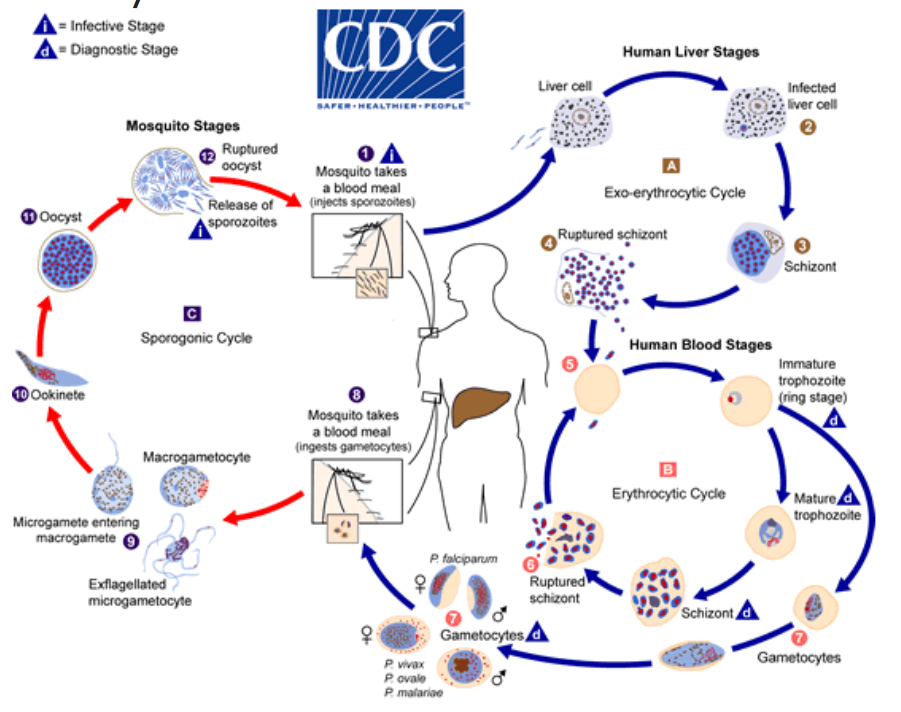
\includegraphics[width=0.7\linewidth]{figures/CDC_malariaCycle.png}
%    \caption{Diagrama esquemático del ciclo de vida del parásito de la malaria.}
%    \label{fig:enlaces}
%\end{figure}


\chapter{Estructura y crecimiento de la hemozoína}



\section{Molécula precursora de la hemozoína}

La hemozoína puede entenderse como un cristal formado a partir de dímeros que se forman a partir de unidades de ferriprotoporfirina IX, también denominada Fe(III)-protoporfirina IX o FP-Fe(III). En consecuencia, para comprender la arquitectura molecular de la hemozoína es necesario analizar primero el origen y las características de esta especie química, ya que constituye la unidad estructural básica a partir de la cual los dímeros desarrollan los procesos posteriores de agregación, nucleación y crecimiento cristalino.\\

La molécula precursora de la ferriprotoporfirina IX es el hemo, un grupo presente en diversas proteínas biológicas, entre ellas la hemoglobina. Estructuralmente, el hemo está formado por un anillo de protoporfirina IX que coordina un ion hierro Fe(II). Dentro de la hemoglobina, este grupo se encuentra protegido por el entorno proteico y participa de manera controlada en procesos de unión y transporte de oxígeno. Sin embargo, cuando la proteína es degradada, el grupo hemo queda expuesto al medio y pierde la estabilización que le proporcionaba la estructura proteica.\\

Una vez liberado de la hemoglobina, el hierro del hemo experimenta una oxidación desde el estado ferroso Fe(II) hacia el estado férrico Fe(III). Como resultado de este proceso se genera la especie conocida como ferrihemo, cuya forma más relevante en el contexto de la hemozoína corresponde a la ferriprotoporfirina IX, es decir, la protoporfirina IX coordinando un hierro en estado de oxidación $+3$. Ese hierro no permanece completamente contenido en el plano del anillo, sino que sobresale parcialmente de él, lo que le da a la molécula un carácter coordinativamente activo. Esta transformación es fundamental porque modifica las propiedades electrónicas y de coordinación del sistema, favoreciendo la interacción entre moléculas vecinas de su misma especie.\\

La importancia de esta etapa radica en que, tanto los modelos clásicos basados en dímeros unidos mediante enlaces hierro-carboxilato, como las propuestas más recientes que incorporan apilamiento $\pi-\pi$ e interacciones supramoleculares complejas, consideran que la cristalización comienza a partir de agregados formados por moléculas individuales de Fe(III)-protoporfirina IX. Por ejemplo, en los trabajos de Pagola et al. y Klonis et al. esta unidad se presenta como la base estructural inmediata tanto de la BH sintética como de la HZ natural \cite{PagolaSilvina2000, Klonis2010}. En consecuencia, la comprensión de la estructura de la hemozoína requiere reconocer que la ferriprotoporfirina IX no es simplemente un precursor químico, sino el bloque de construcción fundamental del cristal.\\

%El hemo es un tipo de molécula que contiene un hierro en el centro de un anillo que se llama porfirina que se encuentra dentro de varias proteinas como un ligando. Cuando el hemo está fuera de la proteina se llama hemina (o hemo libre). Hay varios tipos de hemo que se distinguen por diferentes terminaciones, el  hemo tipo B es el que se encuentra detro de la hemoglobina y el que nos interesa en el proyecto. En la figura \ref{fig:hemo} está representada el hemo libre tipo B (o hemina). 


Desde un punto de vista físico, esta molécula es propensa a agregarse porque combina dos rasgos complementarios: por un lado, un centro metálico capaz de coordinar ligandos oxigenados, y por otro, una superficie aromática plana que favorece el apilamiento entre moléculas vecinas. En la hemozoína, esa dualidad es la que hace posible que un monómero no permanezca aislado, sino que tienda a organizarse en unidades de orden superior. Esa idea está implícita tanto en la interpretación clásica de Pagola et al. como en la reinterpretación moderna de Klonis et al. y en el análisis energético de Marom et al \cite{ Marom2011}.
Puede pensarse en la FP-Fe(III) como una especie de “plataforma” molecular rígida y muy conjugada, capaz de apilarse con otras iguales. En el centro de esa plataforma se encuentra el Fe(III), coordinado por los nitrógenos del anillo porfirínico. Además, la molécula posee dos tipos de sustituyentes laterales que resultan decisivos para su autoensamblaje: los propionatos y los vinilos. Los propionatos son cadenas laterales terminadas en grupo carboxílico, mientras que los vinilos son grupos insaturados más pequeños. Esta disposición aparece de manera explícita en el monómero de la figura \ref{fig:hemina}.\\


\begin{figure}[h!]
    \centering
    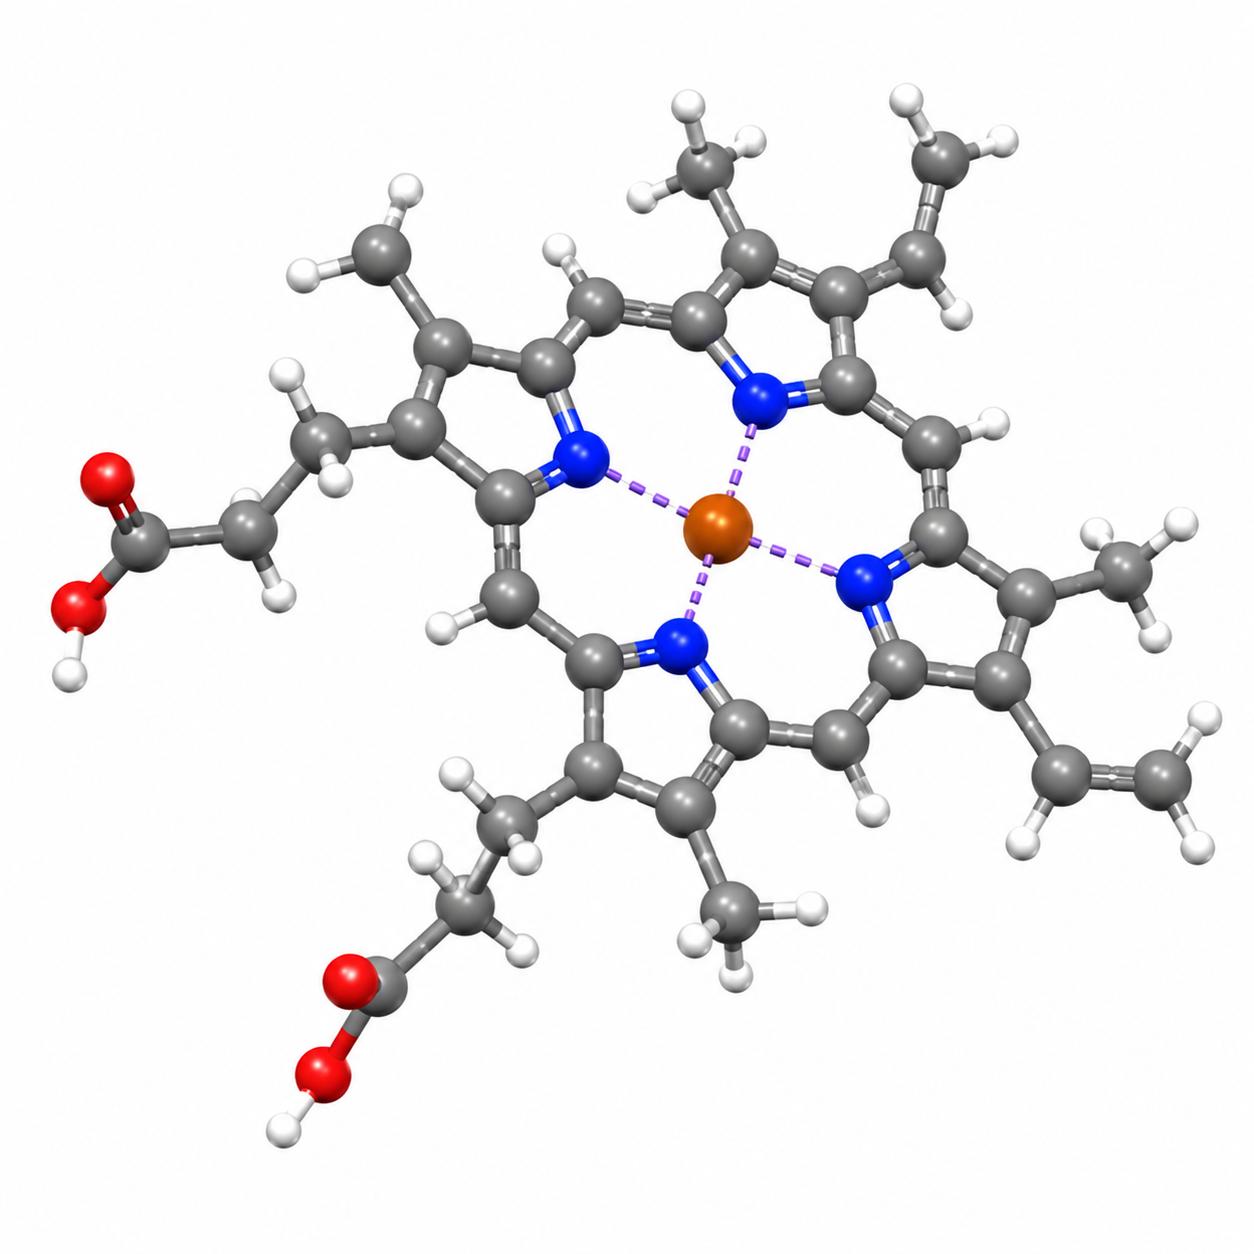
\includegraphics[width=0.5\linewidth]{figures/hemina.png}
    \caption{FP-Fe(III) o Hematina}
    \label{fig:hemina}
\end{figure}\\


%Pagola et al. destacan que el resultado estructural depende de la ubicación de la porfirina y de los grupos vinilo y propionato; Marom et al. muestran, además, que la geometría de esos sustituyentes cambia entre las distintas configuraciones posibles del dímero.\\

%EPAEPAEPAEPAEPA\\

%El grupo hemo (Fe–protoporfirina IX) es una porfirina con alta reactividad oxidativa, derivando en efectos citotóxicos para el parásito. Para evitar este efecto, el parásito lo transforma en hematina (Fe$^{3+}$-protoporfirina IX) y promueve la formación de dímeros estabilizados por interacciones $\mu$-propionato y apilamiento $\pi$-$\pi$ entre unidades de porfirina. Esos dímeros se asocian en láminas que, a su vez, se apilan formando el cristal triclínico conocido como hemozoína, cuyo análogo sintético es la $\beta$-hematina (una fase insoluble, estructuralmente ordenada e inerte desde el punto de vista químico) \cite{Pagola2000}. A partir de esa base estructural, la biocristalización puede descomponerse en etapas que incluyen \textbf{(i)} nucleación, ya sea clásica: aparece primero un núcleo (o semilla) pequeño, esféricamente simétrico, por fluctuaciones de moléculas y, si ese núcleo alcanza

%Diversos medicamentos actúan sobre pasos distintos del proceso de biocristalización. Los quinolínicos (por ejemplo, la cloroquina) se unen al hemo libre y previenen la dimerización $\mu$-propionada que inicia el apilamiento cristalino; otros compuestos (por ejemplo, la quinina) se adsorben sobre caras cristalinas activas, bloqueando sitios de incorporación; algunos agentes modifican el microambiente vacuolar (pH, lípidos) y con ello afectan la probabilidad de nucleación y la estabilidad de agregados precursores; mientras que derivados de la artemisinina inducen daño por radicales libres activados por el hierro del hemo, que puede afectar indirectamente la formación y estabilidad de la hemozoína.  El detalle de estos mecanismos y su eficacia frente a distintas rutas (clásica vs no-clásica) continúa siendo un área activa de investigación.\\


%Dado que la cristalización de hemozoína es un proceso central para la supervivencia del parásito y un blanco molecular de los tratamientos actuales, modelarlo con detalle puede enriquecer la información acerca de: (i) identificar qué sitios superficiales (facetas, bordes, kinks) son críticos para la incorporación; (ii) discriminar mecanismos de inhibición (bloqueo estérico vs alteración termodinámica vs film-forming); y (iii) explorar cómo variaciones en afinidad molecular, movilidad superficial o en protocolos de dosificación afectan la eficacia inhibitoria. Estas preguntas tienen relevancia directa para el diseño racional de compuestos y para proponer estrategias que reduzcan la probabilidad de aparición de resistencias.\\ %\cite{Herrera2023,Herraiz2019}.\\

\section{Unidad de crecimiento y cristalización}\label{sec:GU_cry}


A partir de ahora, se hablará de la química de la BH, teniendo en cuenta que en condiciones químicas iguales, se comporta idénticamente a la HZ. El primer nivel supramolecular de organización aceptado para la BH es el dímero de hematina. En el modelo clásico de Pagola et al., dos moléculas de FP-Fe(III) se enlazan mediante dos interacciones recíprocas Fe\text{-}O (carboxilato): el hierro de una molécula coordina al oxígeno del propionato de la otra, y viceversa, formando el conocido enlace $\mu$-Propionato. Esta interacción genera un dímero centrosimétrico que pasó a ser considerado la unidad repetitiva principal del cristal \cite{PagolaSilvina2000}.\\

%En la nomenclatura posterior de Marom et al., esta especie corresponde al cd11, que es el dímero centrosimétrico más estable y el que domina la fase mayor de $\beta$-hematina.\\

La razón por la cual dos monómeros tienden a formar un dímero no es accidental. En un entorno ácido, y especialmente en condiciones donde el hemo libre se encuentra poco estabilizado por el solvente, los grupos propionato pueden actuar como puntos de unión entre moléculas vecinas. Esto hace que la coordinación Fe\text{–}O sea una ruta natural para reducir la energía local del sistema. Pagola et al. encontraron que, al resolver la estructura de la BH, las moléculas se organizaban precisamente en pares unidos por dos enlaces hierro–carboxilato. Marom et al. reforzaron esta idea al mostrar que, incluso desde un enfoque de primeros principios, la dimerización por carboxilato sigue siendo un paso muy favorable para iniciar la cristalización \cite{PagolaSilvina2000, Marom2011}. En el modelo clásico, estos dímeros no quedan aislados, sino que se enlazan entre sí mediante puentes de hidrógeno entre los grupos propiónicos libres. De este modo, el cristal no se entiende como una cadena lineal de hematina, sino como una red de dímeros cohesionados por interacciones más débiles, pero decisivas para la arquitectura global.\\

%Pagola et al. describen estos enlaces de hidrógeno como el mecanismo que conecta los dímeros en el cristal; Marom et al. añaden que, al considerar el cristal completo, los grupos propiónicos quedan más extendidos y la geometría del dímero se ajusta mejor al entorno cristalino.\\

Conviene subrayar que este dímero no debe imaginarse como una unión puramente geométrica o superficial. Se trata de una asociación en la que la coordinación metal–oxígeno tiene un papel central, y donde el estado del hierro, la orientación de los propionatos y la planitud relativa de los anillos porfirínicos determinan la estabilidad del conjunto. Ese es precisamente el motivo por el cual la estructura del dímero ha sido objeto de revisión en trabajos posteriores. Klonis et al. señalan que, junto con el dímero clásico formado por enlaces $\mu$-Propionato, existen además contactos con mayor solapamiento $\pi$ entre los anillos porfirínicos \cite{Klonis2010}, y Marom et al. muestran que la estabilidad del dímero depende fuertemente de la dispersión y del entorno cristalino \cite{Marom2011}.\\

%Aun así, el dímero cíclico sigue siendo el punto de partida estructural más sólido para describir la hemozoína.\\

%Una vez que se forma el dímero inicial de hemo, el problema deja de ser puramente molecular y pasa a ser supramolecular: cómo se ordenan esas unidades entre sí para generar el cristal. En la visión clásica de Pagola et al., la hemozoína se entiende como una red de dímeros cíclicos que se enlazan entre sí por puentes de hidrógeno entre los grupos propiónicos no coordinados. En esa imagen, el dímero es la unidad estructural básica, y el cristal surge por repetición ordenada de ese motivo en una red tridimensional. Esta interpretación se apoya en el refinamiento estructural de la $\beta$-hematina, donde se observa que las moléculas se agrupan en pares mediante enlaces Fe–carboxilato, y luego esos pares se conectan por interacciones de hidrógeno.\\

Además, los estudios de Klonis et al. también mostraron que la descripción clásica podría estar incompleta. A partir del reanálisis estructural de hemozoína natural, propusieron que el cristal no debe imaginarse solo como un conjunto de dímeros de tipo $\mu$-Pr, sino como una estructura donde también son relevantes otros dos modos de asociación entre moléculas de hematina: el dímero $\pi-\pi$ y la interacción tipo P. En su propuesta, a diferencia de los enfoques clásicos, los dímeros $\pi-\pi$ son considerados como la unidad de crecimiento de la estructura cristalina final. Dos moléculas de hematina pueden acercarse con sus anillos porfirínicos planos casi paralelos, de forma que exista un solapamiento importante de las nubes $\pi$. Esa superposición no es un enlace covalente; es una interacción de apilamiento aromático que aporta estabilidad por dispersión y por complementariedad geométrica. Klonis et al. insisten en que, en este dímero, el solapamiento de los anillos es mucho mayor que en el $\mu$-Pr. Además, los grupos vinilo también contribuyen al contacto. Por eso proponen que el dímero $\pi-\pi$  es un mejor candidato para la unidad de nucleación de la BH \cite{Klonis2010} . En la figura \ref{fig:comparacion_hemo} se observa una comparación entre las dos propuestas de formación de los dímeros que conforman la unidad de crecimiento básica de la BH, y por ende de la HZ.\\


\begin{figure}[h!]
    \centering

    \begin{subfigure}{0.5\textwidth}
        \centering
        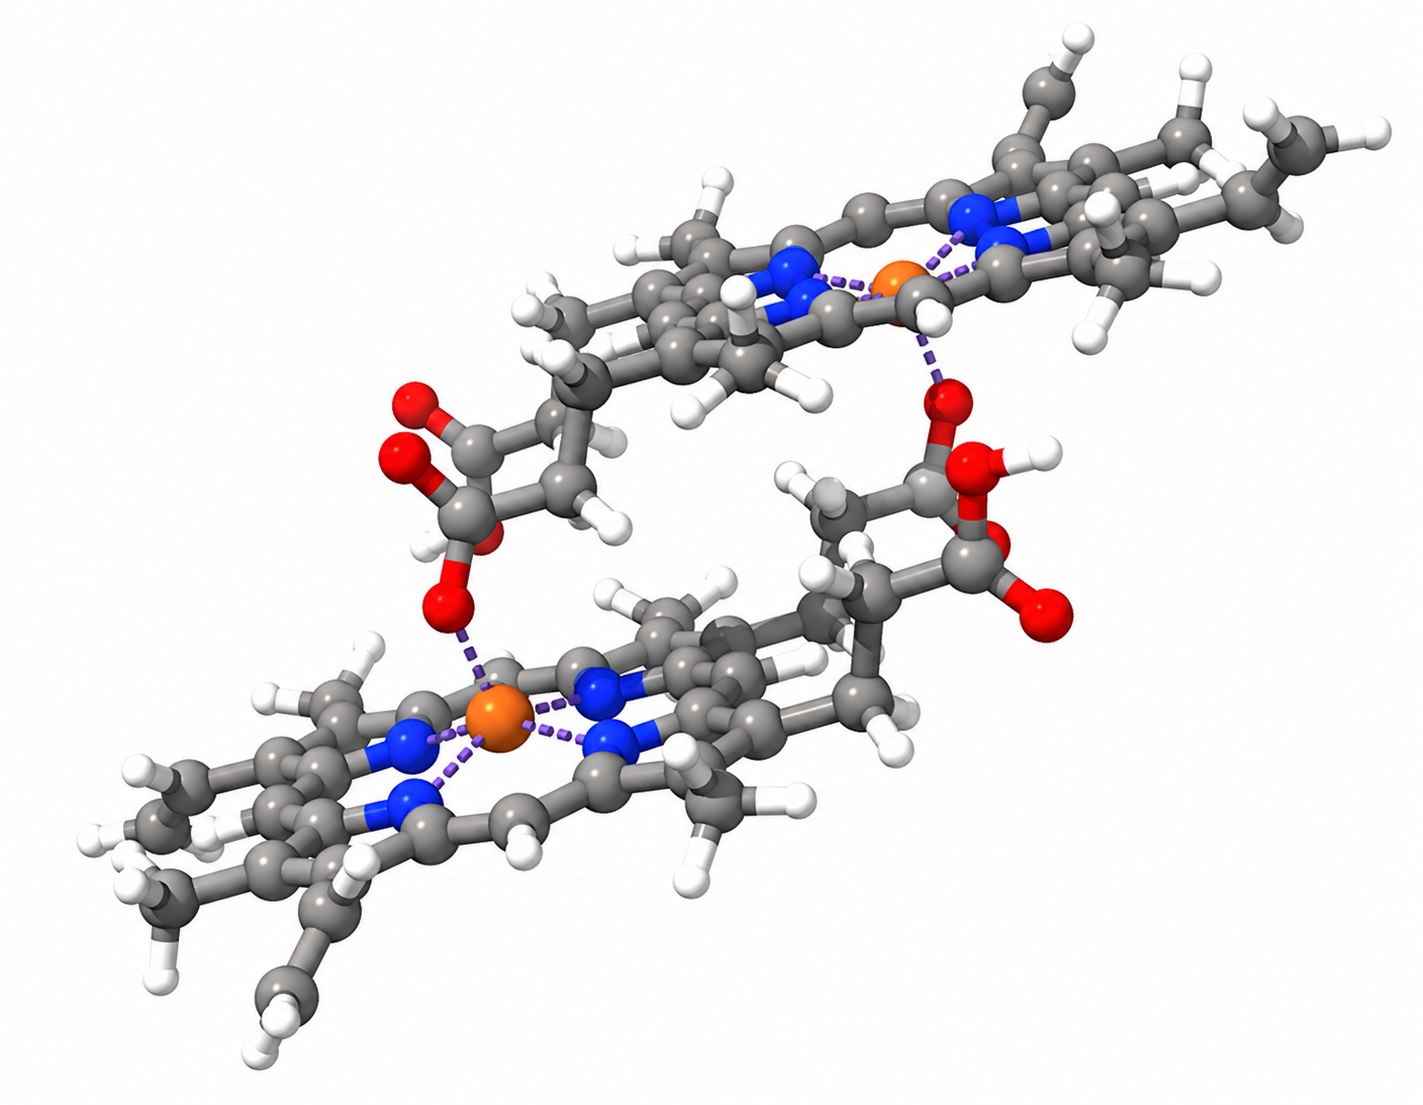
\includegraphics[width=\linewidth]{figures/GU_mPr.png}
        \caption{Unidad de crecimiento a partir de dímeros formados con enlaces $\mu$-Pr.}
        \label{subfig:muPr}
    \end{subfigure}
    \hfill
    \begin{subfigure}{0.45\textwidth}
        \centering
        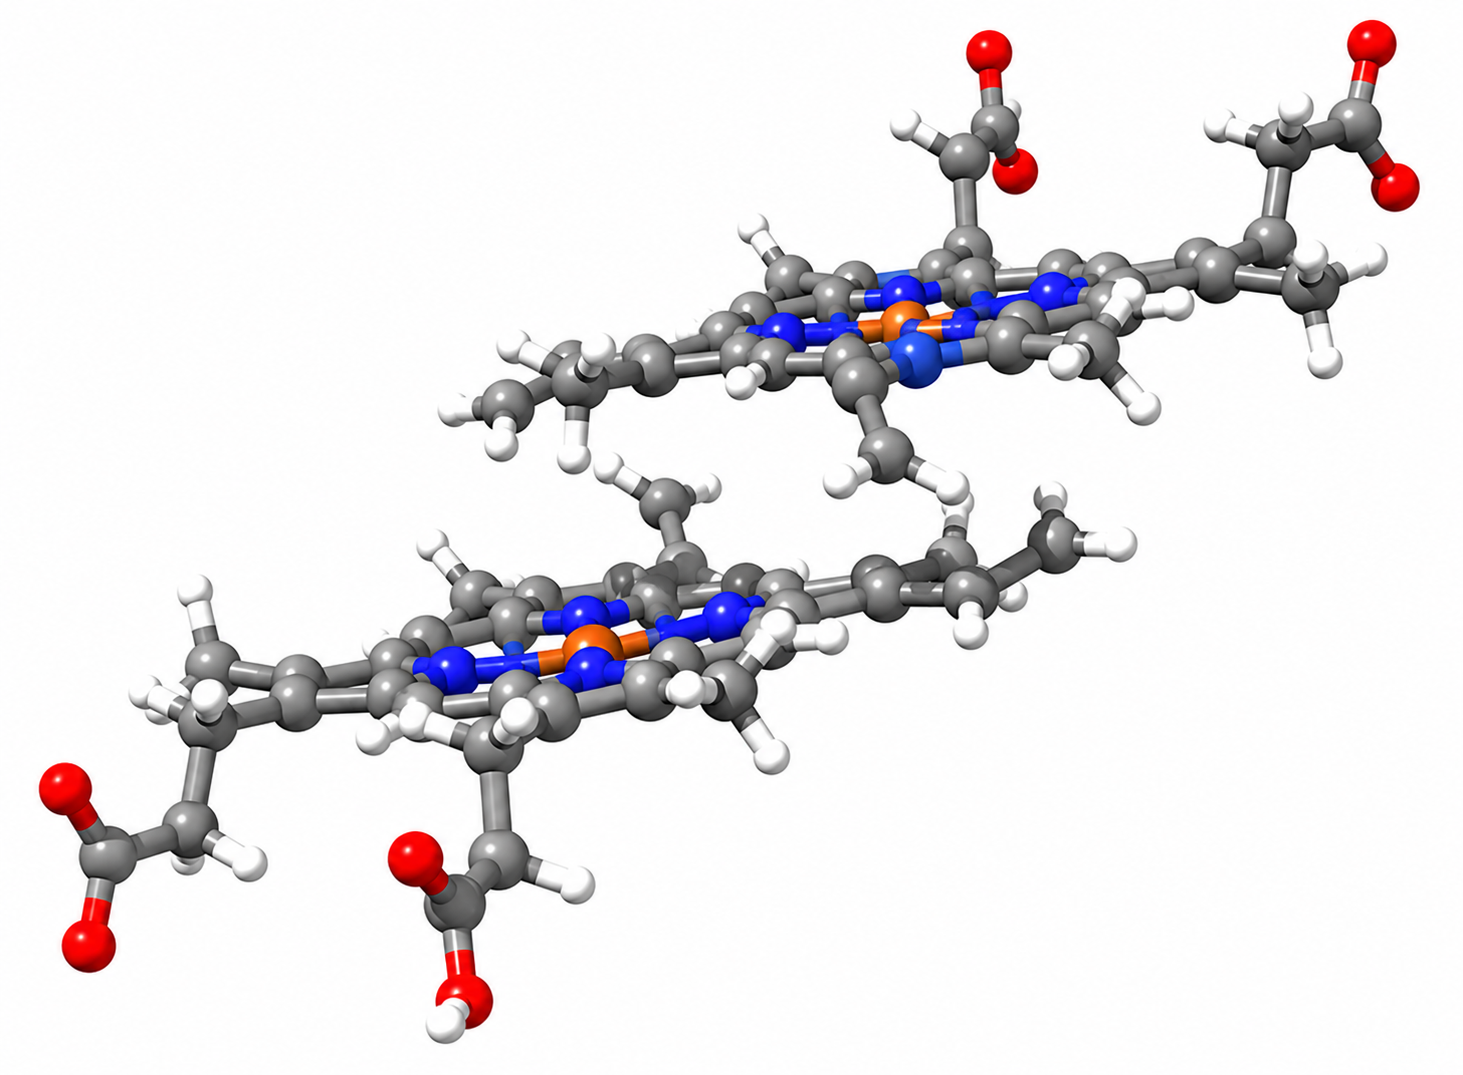
\includegraphics[width=\linewidth]{figures/GU_pp.png}
        \caption{Unidad de crecimiento a partir de dímeros formados con interacciones $\pi-\pi$.}
        \label{subfig:pipi}
    \end{subfigure}

    \caption{Comparación entre las dos propuestas de dímeros formadores de hemozoína o $\beta$-hematina.}
    \label{fig:comparacion_hemo}
\end{figure}\\

Por su parte, las interacciones tipo P se pueden explicar como un contacto desplazado y asimétrico. Cada molécula de hematina conserva una orientación general similar a la de su vecino, pero las moléculas están corridas una respecto de la otra. En este contacto no domina ni el solapamiento completo $\pi-\pi$ ni la coordinación hierro–carboxilato: lo que aparece es una cadena extendida, donde cada monómero aporta sus extremos vinilo y propionato a dos vecinos distintos. Klonis lo presenta como una interacción que sirve para extender columnas de dímeros $\pi-\pi$. Es decir, la interacción tipo P no sería la unidad de nucleación, sino el mecanismo que permite que los dímeros se organicen en agregados lineales más grandes \cite{Klonis2010}. La figura \ref{fig:P-Type} muestra un esquema de la interacción.\\

\begin{figure}[h!]
    \centering
    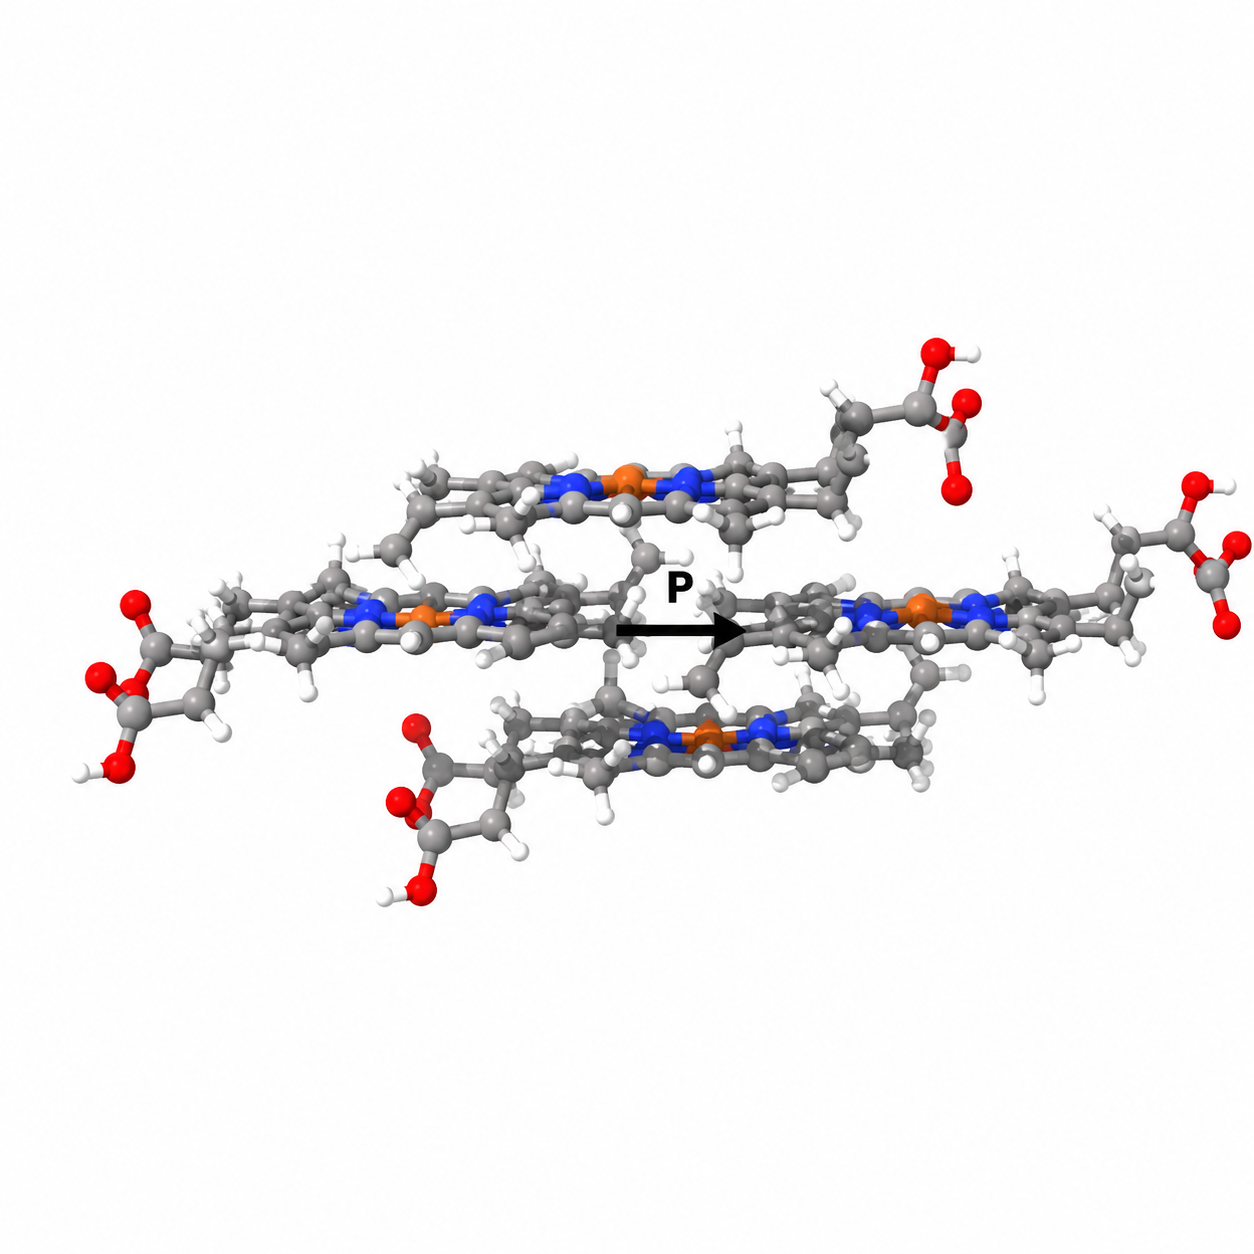
\includegraphics[width=0.5\linewidth]{figures/Ptype.png}
    \caption{Interacción de tipo P entre dos dímeros $\pi-\pi$.}
    \label{fig:P-Type}
\end{figure}\\

Por otro lado, cuando los dímeros formados a partir de interacciones $\pi-\pi$ coexisten, se pueden dar enlaces $\mu$-Pr entre los iones de hierro y los propionatos libres de diferentes dímeros, como se muestra en la figura \ref{fig:muPr y pipi}. Dando paso a la formación de cadenas compuestas de dímeros $\pi-\pi$ unidos por enlaces $\mu$-Pr, dando un giro de tuerca a la comprensión clásica de la formación final de los cristales de BH.\\

\begin{figure}[h!]
    \centering
    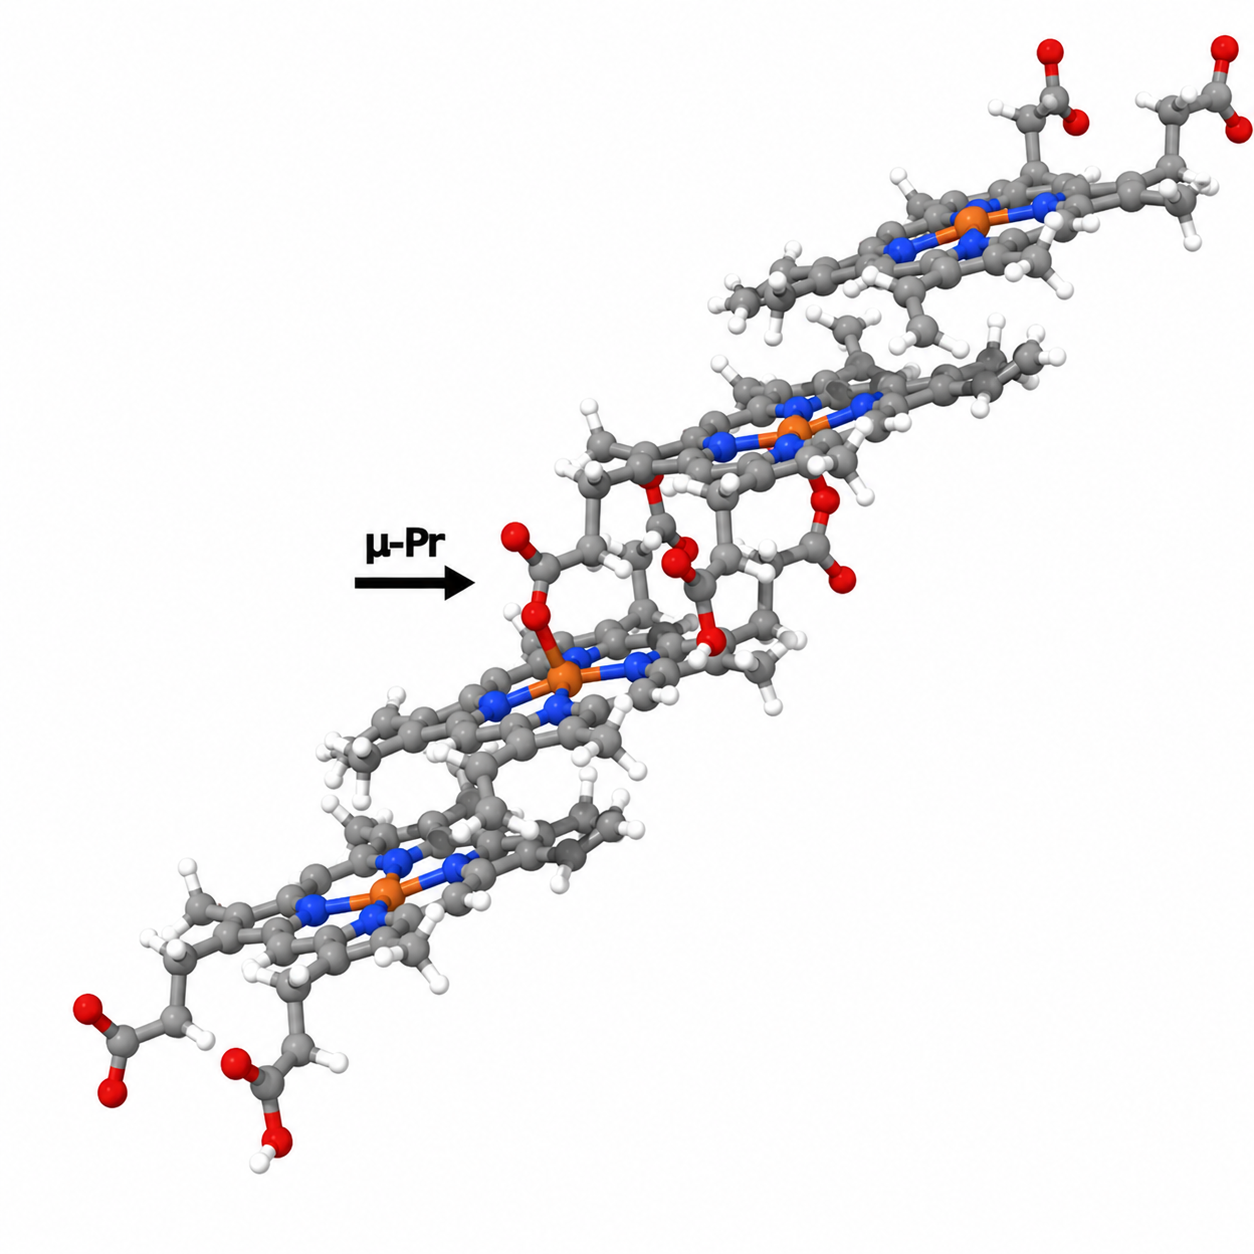
\includegraphics[width=0.5\linewidth]{figures/mPr.png}
    \caption{Enlace $\mu$-Pr de dos dímeros $\pi-\pi$.}
    \label{fig:muPr y pipi}
\end{figure}\\

Otro tipo de interacción fundamental para el resultado final del cristal de BH son los puentes de Hidrógeno. Se puede observar esta interacción en la figura \ref{fig:enlaces_HB}. Estas aparecen cuando los grupos propiónicos que no están coordinados al hierro quedan libres para interaccionar con propionatos vecinos. En Pagola, ya se veía que esos grupos conectan los dímeros en una red cristalina \cite{PagolaSilvina2000}. Klonis retoma esa idea y la coloca en un nivel más amplio: los grupos carboxílicos libres entrecruzan las láminas y ayudan a fijar el cristal. En su modelo de crecimiento, los enlaces de hidrógeno no forman el núcleo inicial, pero sí son cruciales para el empaquetamiento final: actúan como un sistema de “amarre” que estabiliza las láminas y evita que el cristal se desarme \cite{Klonis2010}. Marom et al. también confirman que la estabilización por enlaces de Hidrógeno es relevante, especialmente a lo largo de la dirección cristalográfica donde dominan esas conexiones \cite{Marom2011}.\\

\begin{figure}[h!]
    \centering
    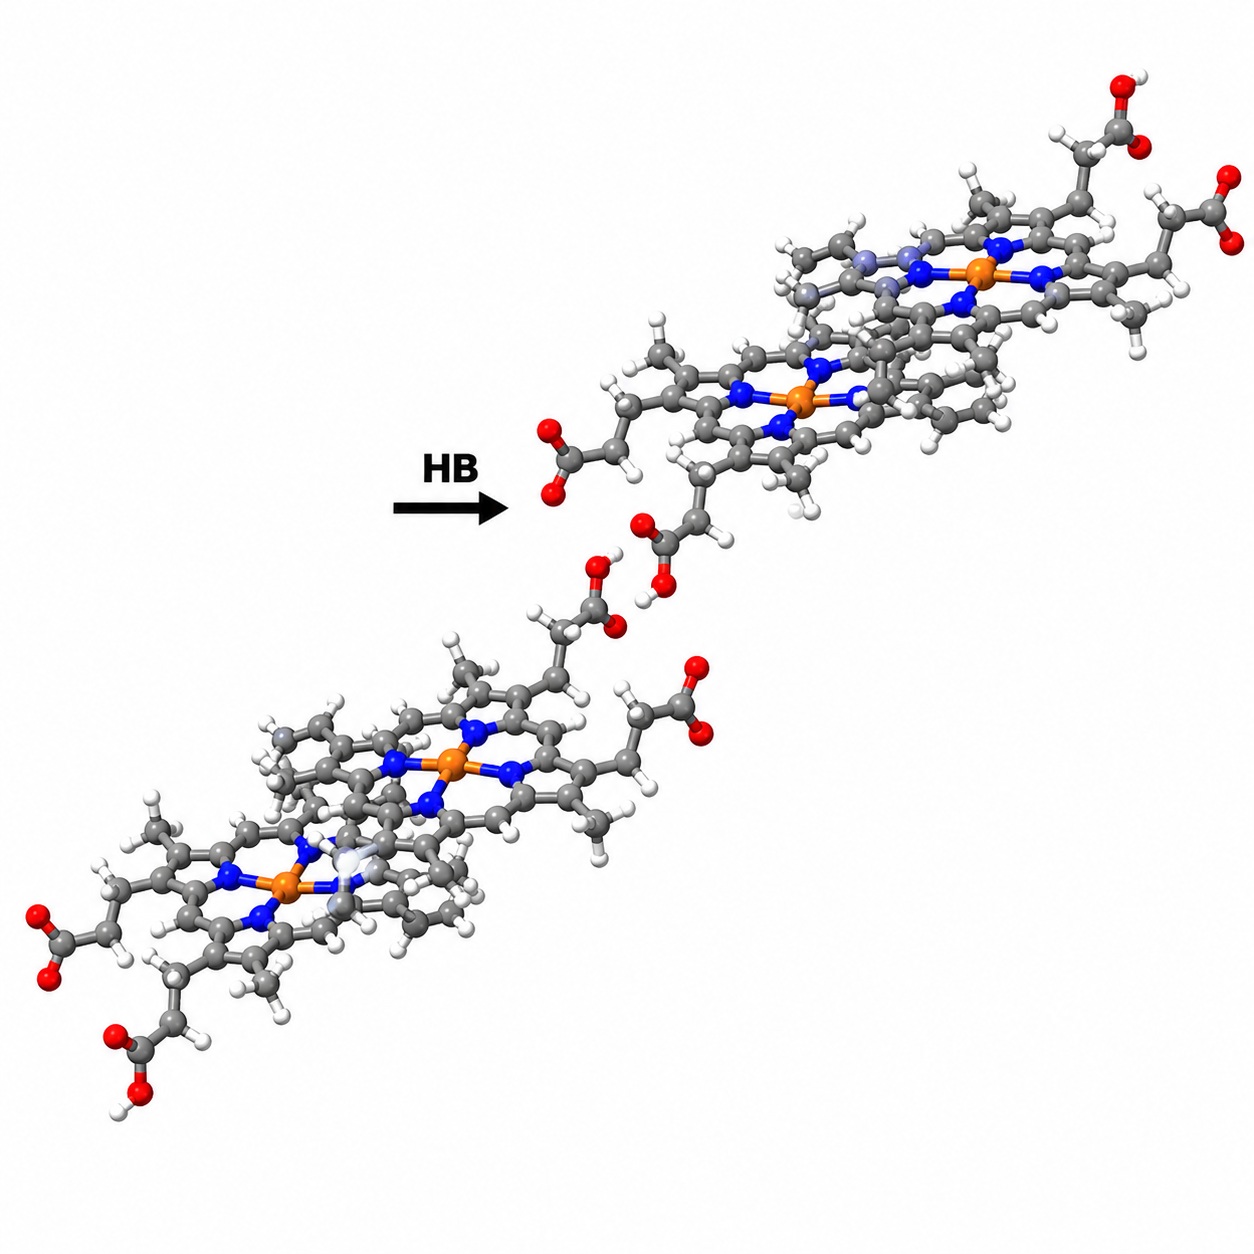
\includegraphics[width=0.5\linewidth]{figures/HB.png}
    \caption{Enlaces o puentes de Hidrógeno}
    \label{fig:enlaces_HB}
\end{figure}\\

Por lo tanto, aunque los estudios clásicos proponen los dímeros formados a partir de $\mu$-Pr como la unidad de crecimiento para la BH, y que estos dímeros después formaban su estructura cristalina a partir de enlaces de Hidrógeno, Klonis objeta que el $\mu$-Pr tiene muy poco o ningún solapamiento entre porfirinas y está estabilizado casi exclusivamente por el enlace hierro–carboxilato. En un medio acuoso, esa estabilización sería menos favorable. Además, ellos señalan que esa geometría no explica bien la presencia de actividad redox en la superficie del cristal \cite{Klonis2010}. El dímero $\pi-\pi$, en cambio, tiene más solapamiento porfirínico, mayor proximidad entre los macroanillos y, por tanto, una estabilidad mejor justificada en medio acuoso. Klonis añade que el dímero $\pi-\pi$ puede ser la especie predominante de FP-Fe(III) en solución, lo que lo vuelve un candidato más plausible como nucleante inicial. La evidencia que presentan Klonis et al. en su estudio no es una prueba directa de nucleación, sino una convergencia de indicios. Sin embargo, sus detalles se escapan del objetivo de este trabajo.\\

Lo que me gustaría rescatar del enfoque presentado en Klonis, es que la ruta que siguen los cristales de BH para su formación final, difiere en algunos detalles respecto a la descripción clásica, pues en su propuesta hay una ruta de ensamblaje jerárquica concreta, que se podría resumir así: \\

\begin{enumerate}
    \item \textbf{Nucleación inicial:} se forman dímeros $\pi-\pi$.
    \item \textbf{Crecimiento unidimensional:}  esos dímeros se agrupan en columnas mediante interacciones tipo P.
    \item \textbf{Crecimiento bidimensional:} las columnas se conectan lateralmente por enlaces $\mu$-Pr, formando una lámina.
    \item \textbf{Crecimiento tridimensional:} las láminas se apilan y se estabilizan por fuerzas de van der Waals y puentes de hidrógeno entre grupos propiónicos no coordinados de láminas adyacentes.
\end{enumerate} \\

La forma resultante es la de un cristal hecho de láminas de grosor cercano a 11 Å, donde las interacciones fuertes y débiles están repartidas por niveles La figura \ref{fig:formacion} muestra un esquema de la formación de las láminas 2D. No obstante, cabe aclarar que en Klonis et al. cada lámina puede verse desde dos lecturas equivalentes: como una colección de dímeros $\mu$-Pr unidos por $\pi-\pi$ o como una colección de dímeros $\pi-\pi$ conectados por $\mu$-Pr. Esa dualidad es precisamente la señal de que el cristal no es trivial y de que la estructura depende de cómo uno elija la unidad repetitiva \cite{Klonis2010}.\\

Así, la organización supramolecular de la hemozoína puede resumirse como una estructura en la que el dímero sigue siendo esencial, pero la forma concreta de empaquetamiento cristalino no es única ni trivial. La imagen moderna es la de un material donde coexisten coordinación metal–carboxilato, apilamiento aromático, enlaces de hidrógeno y fuerzas de dispersión, todas actuando de manera concertada. Esta visión es más rica que la clásica, porque permite entender no solo la estructura global, sino también la reactividad superficial y la posible heterogeneidad del cristal natural. En este trabajo, optamos por la formación a partir de dímeros $\pi-\pi$ como la unidad de crecimiento del modelo desarrollado.\\

\begin{figure}[h!]
    \centering
    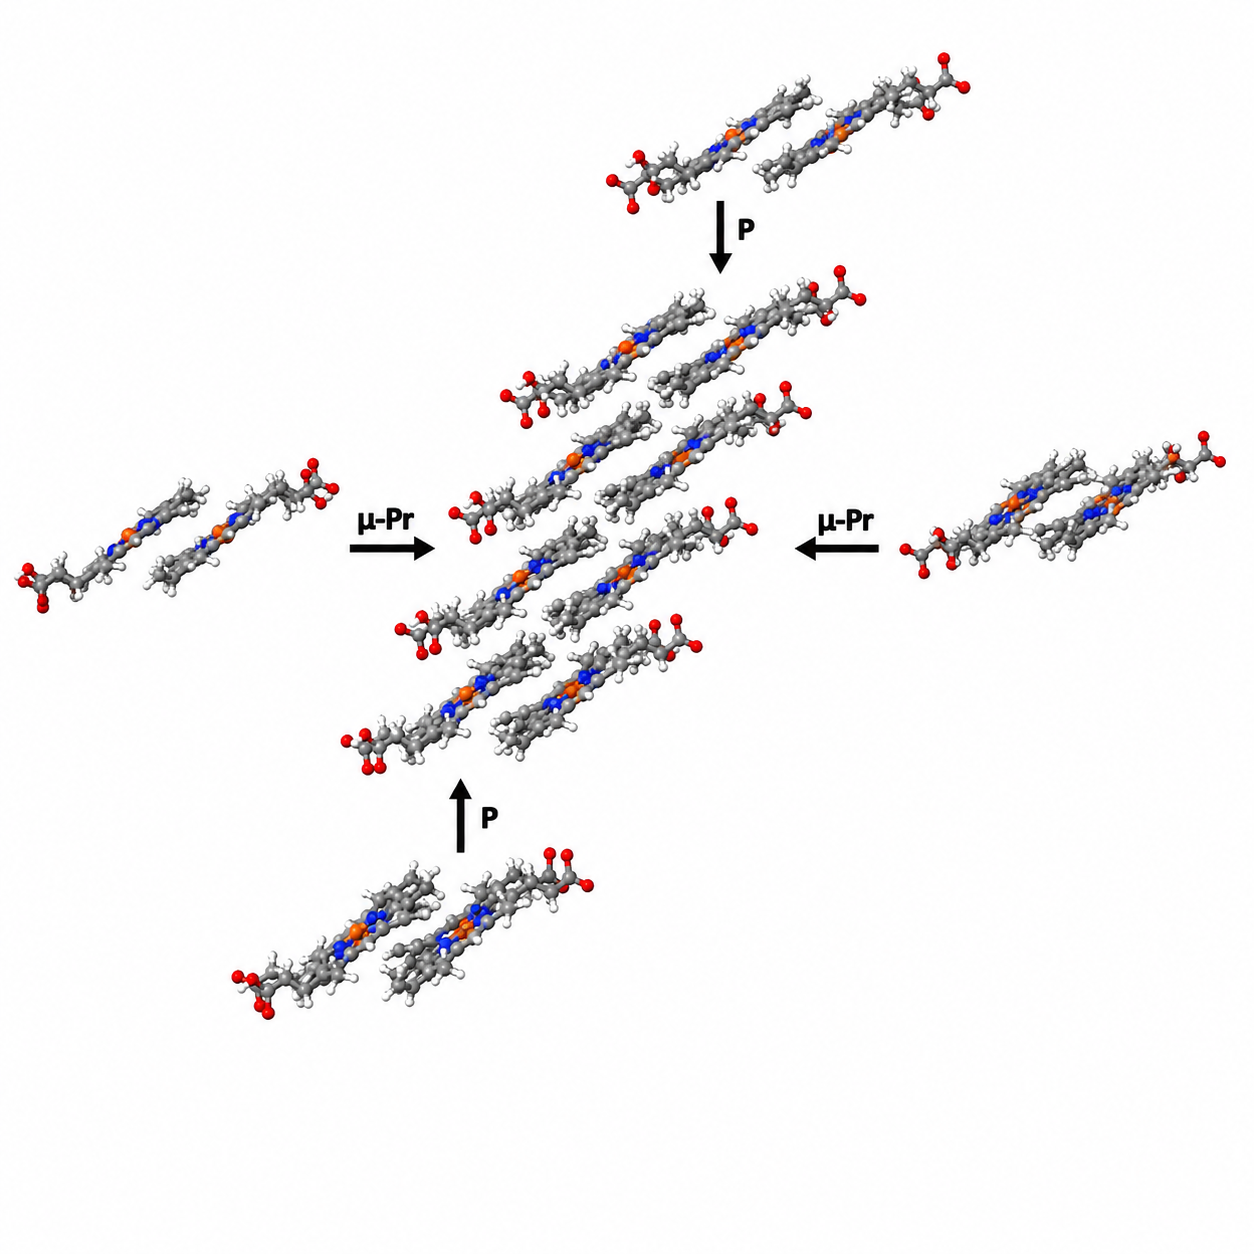
\includegraphics[width=0.65\linewidth]{figures/laywe.png}
    \caption{Formacion de dimeros $\pi-\pi$ seguido de columnas por interacciones tipo P y finalmente láminas 2D por enlaces $\mu$-Pr.}
    \label{fig:formacion}
\end{figure}\\

\section{Nucleación y crecimiento de la hemozoína}


Ahora bien, pese a la descripción anterior de la estructura y los pasos químicos que sigue la hematina para convertirse en BH, la cristalización de ferrihemo en medio acuoso y ácido no se limita simplemente a la ejecución ordenada de dichos pasos, sino que además de la formación de estas especies precursoras, requiere la aparición de núcleos estables y el posterior crecimiento cristalino.\\

%\cite{Pasternack1993}.\\

Desde un punto de vista cinético, la evolución temporal de la cristalización está gobernada por la competencia entre procesos de asociación molecular, nucleación y crecimiento. Como consecuencia, las curvas experimentales de formación de BH presentan típicamente una forma sigmoidal, caracterizada por una etapa inicial lenta, una región de crecimiento acelerado y una saturación final asociada al agotamiento del material disponible para cristalizar. En esta sección, revisaremos algunos conceptos básicos que explican este proceso, así como algunos modelos clásicos y la propuesta moderna hecha por Parra en su tesis de maestría \cite{AlirioParra2023}, apoyándome en la revisión de alguna literatura fundamental que se referencia en su trabajo.\\

%\cite{Pasternack1993}.

\subsection{Teoría clásica de nucleación}

La descripción más ampliamente utilizada para estudiar la formación de cristales en solución es la teoría clásica de nucleación (CNT, por sus siglas en inglés). En este formalismo se considera que los núcleos cristalinos son agregados microscópicos de la nueva fase que poseen las mismas propiedades estructurales que el cristal macroscópico. La estabilidad de dichos núcleos surge de la competencia entre una contribución energética favorable asociada al volumen cristalino y una contribución desfavorable asociada a la superficie del agregado \cite{Erdemir2009}.\\

La variación de la energía libre de Gibbs asociada a la formación de un núcleo esférico de radio $r$ puede expresarse como\\

\begin{equation}
\Delta G(r)
=
-\frac{4}{3}\pi r^{3}\Delta G_{V}
+
4\pi r^{2}\gamma ,
\label{eq:cnt}
\end{equation}\\

\noindent donde $\Delta G_{V}$ representa la diferencia de energía libre por unidad de volumen entre la fase cristalina y la solución, mientras que $\gamma$ corresponde a la energía interfacial entre ambas fases.\\

El primer término favorece la formación del cristal, mientras que el segundo penaliza la creación de superficie. Como resultado, existe un tamaño crítico para que el núcleo sea estable, obtenido al maximizar la energía libre:\\

\begin{equation}
r^{*}
=
\frac{2\gamma}{\Delta G_{V}}.
\label{eq:r_critico}
\end{equation}\\

Los agregados con radios inferiores a $r^{*}$ son termodinámicamente inestables y tienden a redisolverse en la solución. Por el contrario, aquellos que superan dicho tamaño crítico se vuelven estables y pueden crecer espontáneamente mediante la incorporación de nuevas unidades estructurales \cite{Erdemir2009}.\\

%En el contexto de la formación de hemozoína, esta barrera de nucleación determina el tiempo de inducción observado al comienzo de las curvas experimentales de cristalización \cite{Parra2024}.

%\subsubsection{Formación de especies precursoras}

%Aunque la teoría clásica de nucleación proporciona una descripción adecuada del crecimiento cristalino, diversos estudios han mostrado que la cristalización de ferrihemo involucra etapas previas de autoensamblaje molecular \cite{Klonis2002,Stiebler2014}.

%En solución, las moléculas de hemo presentan una marcada tendencia a asociarse mediante interacciones entre sus anillos porfirínicos. Klonis y colaboradores propusieron que esta autoasociación conduce inicialmente a la formación de dímeros apilados de tipo $\pi$-$\pi$ \cite{Klonis2002}. Estas especies representan estados intermedios que preceden a la formación de las unidades estructurales características de la $\beta$-hematina.

%Posteriormente, dichos agregados experimentan una reorganización molecular que conduce a la formación de dímeros $\mu$-propionato, considerados los bloques fundamentales para la construcción del cristal \cite{Parra2024}. Desde esta perspectiva, la cristalización de BH no consiste simplemente en la agregación de moléculas individuales de hemo, sino en la generación previa de unidades precursoras adecuadas para la nucleación.

%Stiebler y colaboradores sugirieron que la etapa limitante del proceso está relacionada con la baja solubilidad del ferrihemo en medio ácido, lo que dificulta la formación de los enlaces necesarios para la generación de los dímeros cristalinos \cite{Stiebler2014}. En contraste, el modelo propuesto por Parra considera que la conversión entre los dímeros $\pi$-$\pi$ y los dímeros $\mu$-propionato constituye el verdadero paso limitante de la cinética global \cite{Parra2024}.

\subsection{Modelos cinéticos de Avrami y Pasternack}

Entre los modelos estudiados por Parra para describir estos procesos de cristalización a partir de la nucleación, se encuentra la ecuación de Avrami, originalmente desarrollada para estudiar transformaciones de fase gobernadas por nucleación y crecimiento cristalino.\\

El modelo de Avrami surge a partir de la CNT y supone que la velocidad de transformación depende de la aparición de núcleos estables y del crecimiento de estos dentro del material. La fracción transformada puede expresarse como\\

\begin{equation}
X(t)
=
X_0
\left[
1-\exp\left(-kt^{n}\right)
\right],
\label{eq:avrami}
\end{equation}\\

\noindent donde $X_0$ representa la cantidad total de material transformable, $k$ es una constante cinética efectiva y $n$ es el denominado exponente de Avrami.\\

El parámetro $n$ contiene información acerca del mecanismo físico responsable de la transformación. En términos generales, puede escribirse como\\

\begin{equation}
n=n_d+n_N,
\end{equation}\\

\noindent donde $n_d$ está relacionado con la dimensionalidad del crecimiento cristalino y $n_N$ describe el modo de nucleación. Por ejemplo, valores de $n_d=1$, $2$ y $3$ corresponden a crecimiento predominantemente unidimensional, bidimensional y tridimensional, respectivamente. Asimismo, la nucleación instantánea y la nucleación continua producen contribuciones distintas al exponente total \cite{AlirioParra2023}.\\

La principal ventaja del modelo de Avrami es que incorpora de forma natural los dos elementos fundamentales de la cristalización: nucleación y crecimiento. Como consecuencia, reproduce adecuadamente las curvas sigmoidales observadas experimentalmente en numerosos sistemas cristalinos, incluyendo la formación de BH.\\

Sin embargo, el modelo presenta una limitación cuando se aplica a la cristalización de HZ. La ecuación de Avrami supone implícitamente que las unidades básicas necesarias para el crecimiento cristalino ya están presentes en el sistema. En otras palabras, el modelo comienza su descripción cuando el material se encuentra listo para nuclear y crecer, sin considerar las etapas moleculares previas necesarias para formar dichas unidades estructurales \cite{AlirioParra2023}.\\%Por ende, esta limitación motivó el desarrollo de modelos más específicos para la formación de HZ.\\

Por otro lado, diversos estudios experimentales mostraron que las curvas de formación de BH presentan una naturaleza bifásica que no siempre puede describirse adecuadamente mediante una única ecuación de Avrami \cite{Pasternack1993}.\\

Con el fin de representar este comportamiento, Pasternack et al. propusieron un modelo fenomenológico que combina una contribución tipo Avrami con una contribución exponencial simple:\\

\begin{equation}
X(t)
=
y_0
-
y_1
\exp\left(-kt^{n}\right)
-
y_2
\exp\left(-k_s t\right),
\label{eq:pasternack}
\end{equation}\\

\noindent donde $X(t)$ representa la conversión total de hematina en BH.\\

En esta formulación, el primer término exponencial corresponde a un proceso rápido asociado a nucleación y crecimiento cristalino, mientras que el segundo término describe una contribución más lenta cuya naturaleza física no fue establecida explícitamente por los autores \cite{Pasternack1993}. Por lo tanto, el modelo de Pasternack sigue siendo esencialmente fenomenológico. Aunque describe adecuadamente las curvas experimentales, sus parámetros no poseen una interpretación microscópica única. En particular, el término exponencial lento se introduce para mejorar la calidad del ajuste, pero no se deriva de un mecanismo molecular específico de formación de BH.\\

%La introducción de ambas escalas temporales permitió reproducir con gran precisión los datos experimentales disponibles. Desde un punto de vista matemático, el modelo puede interpretarse como una extensión empírica de la ecuación de Avrami capaz de capturar desviaciones respecto al comportamiento sigmoidal ideal.


\subsection{Modelo cinético de dos etapas}

Bajo esta interpretación y con todo lo anterior en mente, el estudio de Parra propone un modelo en el que, efectivamente, la cristalización de BH puede describirse mediante dos procesos consecutivos \cite{AlirioParra2023}.\\

La primera etapa corresponde a la formación de los dímeros a partir de especies precursoras presentes en solución. Este proceso puede representarse mediante una cinética de segundo orden:\\

\begin{equation}
\frac{dX}{dt}
=
k_{1}
(\alpha-X)^{2},
\label{eq:segundo_orden}
\end{equation}\\

\noindent donde $X$ representa la cantidad de dímeros formados, también llamado porcentaje de conversión, $\alpha$ es la cantidad máxima de material convertible y $k_{1}$ es la constante cinética asociada a la formación del precursor \cite{AlirioParra2023}.\\

La solución de la ecuación (\ref{eq:segundo_orden}) es\\

\begin{equation}
X(t)
=
\alpha
-
\frac{\alpha}
{\alpha k_{1} t +1}.
\label{eq:sol_segundo_orden}
\end{equation}\\

Una vez se han generado suficientes dímeros, comienza la segunda etapa, correspondiente a la nucleación efectiva y al crecimiento del cristal. Esta fase puede modelarse mediante una ecuación logística:\\

\begin{equation}
\frac{dX}{dt}
=
k_{2}
X(\beta-X),
\label{eq:logistica}
\end{equation}\\

\noindent donde $\beta$ representa la cantidad máxima de material cristalizable y $k_{2}$ la constante de crecimiento cristalino. La solución correspondiente es\\

\begin{equation}
X(t)
=
\frac{\beta}
{1+\exp\left(-\beta k_{2} t + D\right)},
\label{eq:sol_logistica}
\end{equation}\\

\noindent siendo $D$ una constante determinada por las condiciones iniciales.\\

Finalmente, la cinética global puede expresarse como la suma de ambas contribuciones:\\

\begin{equation}
X(t)
=
\alpha
-
\frac{\alpha}
{\alpha k_{1} t+1}
+
\frac{\beta}
{1+\exp\left(-\beta k_{2} t+D\right)}.
\label{eq:modelo_global}
\end{equation}\\

Esta formulación permite interpretar físicamente la curva de cristalización observada experimentalmente. El primer término describe la generación progresiva de las unidades precursoras necesarias para la nucleación, mientras que el segundo representa el crecimiento cooperativo del cristal una vez se han formado núcleos estables.\\

Aunque hay algunas descripciones no clásicas para la nucleación y crecimiento de cristales en solución, que proponen un paso adicional a partir de la unión de precursores mediante clusters lipídicos, y que estas descripciones han ido tomando bastante fuerza por observaciones experimentales, en este trabajo se utiliza la CNT para reproducir la cinética de crecimiento de la BH.\\

%\subsubsection{Crecimiento cristalino y evolución temporal}

%Una consecuencia directa de este mecanismo es la aparición de curvas de cristalización sigmoidal. Durante los primeros instantes domina la formación de precursores y la velocidad global es relativamente baja. A medida que aumenta la concentración de dímeros $\mu$-propionato y aparecen núcleos estables, la velocidad de crecimiento aumenta significativamente debido a la disponibilidad creciente de superficies cristalinas activas.

%Finalmente, el proceso entra en una región de saturación cuando la cantidad de ferrihemo libre disminuye y la incorporación de nuevas unidades estructurales se vuelve progresivamente menos eficiente.

%Este comportamiento ha sido observado tanto en sistemas acuosos como en medios que contienen componentes orgánicos. En particular, la presencia de interfaces agua-lípido favorece la formación de especies precursoras y acelera considerablemente la cristalización, lo que sugiere que el entorno lipídico presente en la vacuola digestiva del parásito desempeña un papel fundamental en la biomineralización de la hemozoína \cite{Parra2024,Pasternack1993,Stiebler2014}.

En conjunto, la evidencia experimental y teórica disponible indica que la formación de BH es un proceso jerárquico de autoensamblaje molecular en el que la generación de especies precursoras, la nucleación y el crecimiento cristalino están acoplados. Esta visión proporciona un marco físico consistente para interpretar tanto la cinética de formación de BH como los mecanismos mediante los cuales distintos compuestos antimaláricos interfieren con dicho proceso.\\

%Esta secuencia aparece explícitamente en la discusión de Klonis et al. en las pp. 3–4, y constituye una reinterpretación importante del empaquetamiento cristalino.\\

%Desde este punto de vista, el cristal de hemozoína ya no es una estructura gobernada por una sola interacción dominante, sino por una jerarquía de interacciones. En el nivel más fuerte está la coordinación Fe–O(carboxilato) que define el dímero; en el nivel siguiente aparecen los puentes de hidrógeno entre grupos propiónicos libres; y en un nivel más amplio actúan el apilamiento $\pi-\pi$, las interacciones P-type y las fuerzas de dispersión entre sustituyentes laterales. La consecuencia conceptual es importante: la estabilidad del cristal depende tanto de la química de coordinación como del modo en que se acomodan los anillos porfirínicos unos respecto de otros.\\


%Cuando el hemo esta en la hemoglobina su hierro está en estado de oxidación +2 (se denota Fe(II)) y si enlaza adicionalmente una molecula de dioxigeno O2 entonces dona un electron a la molecula O2 y el hierro pasa a estado de oxidación +3 que se denota Fe(III). Tanto el hemo libre como el ligado a la proteina tienen el mismo estado de oxidacion dependiendo de si estan enlazados a una molecula adicional como por ejemplo O2. Entonces, hemo o hemina sin enlace adicional está en +2 y si se enlaza por ejemplo a un O2 (o un OH) entonces dona un electrón y queda en estado +3. El estado de espin sigue directamente la oxidacion así:
%\begin{itemize}
%    \item Fe neutro: [Ar] 3d$^6$ 4s$^2$ tiene en la capa d 4 electrones no apareados y dos compartiendo un nivel. El momento magnético es $\mu = 4 \mu_B$.
%    \item ion Fe(II): [Ar] 3d$^6$ 4s$^0$ los electrones se donan de la capa s. El momento magnético es $\mu = 4 \mu_B$.
%    \item ion Fe(III): [Ar] 3d$^5$ 4s$^0$ los electrones se donan de la capa s y adicional el que estaba apareado en la capa d. El momento magnético es $\mu = 5 \mu_B$.
%\end{itemize}

%Por evidencia experimental y simulaciones clásicas. En las condiciones de medio acuoso-oleoso el dimero de minima energia libre es un dimero que enlaza por interacción de dispersión los anillos con el "hierro por fuera". Ver isomero 1 en la imagen del articulo de referencia. Este dimero no es el dímero que se propone como el dimero de base de manera estándar pero en el articulo experimental proponen un camino de cristalizacion a partir de estos.


%A nivel molecular, el pigmento se organiza mediante tres modos de autoasociación críticos: \begin{enumerate} \item \textbf{Dímero de metal-propionato ($\mu$-Pr):} Definido por un enlace de coordinación Fe-O recíproco entre el hierro férrico de un monómero y el grupo carboxilato del propionato del compañero. Si bien es el modelo clásico, los datos sugieren que es vulnerable en medios puramente acuosos sin estabilización adicional. \item \textbf{Dímero $\pi$-$\pi$:} Este estado presenta un solapamiento sustantivo de los anillos de porfirina y de los grupos vinilo, estabilizado por fuerzas de Van der Waals. Es el estado predominante del FP-Fe(III) en solución y se considera la unidad estructural de mayor estabilidad inicial. \item \textbf{Interacción Tipo-P (Polimérica):} Una asociación asimétrica donde el extremo propionato y vinilo de una molécula interactúa con la cara coordinada de la siguiente, facilitando la formación de cadenas. \end{enumerate}

%La hemozoína se organiza en una serie de láminas (\textit{sheets}) con un espesor aproximado de 11.0 \AA. Esta arquitectura tridimensional se estabiliza mediante una red cooperativa de fuerzas: \begin{itemize} \item \textbf{Enlaces de Coordinación:} Los enlaces Fe-O reticulan las unidades de hematina dentro de cada lámina. \item \textbf{Interacciones $\pi$-$\pi$:} Cruciales para la estabilización de la estructura extendida y el empaquetamiento compacto de los núcleos de porfirina. \item \textbf{Enlaces de Hidrógeno:} Los grupos de ácido propiónico no coordinados forman puentes de hidrógeno recíprocos con láminas adyacentes, bloqueando la red en su estado cristalino. \item \textbf{Dualidad Reactiva:} El cristal no es totalmente inerte. Presenta una actividad peroxidasa residual del 1.5\% en comparación con el hemo libre. \item \textbf{Interpretación de Datos:} Este 1.5\% de actividad correlaciona precisamente con la proporción de átomos de Fe(III) localizados en la superficie del cristal (asumiendo dimensiones típicas de 100 $\times$ 100 $\times$ 300--500 nm), donde el hierro está parcialmente expuesto al solvente. \item \textbf{Consecuencia Biofísica:} La orientación de los dímeros $\pi$-$\pi$ en las caras expuestas permite que el cristal participe en reacciones de oxidación lipídica, explicando su potencial inmunomodulador. \end{itemize}


\chapter{Método Monte Carlo cinético}

\section{Un poco de teoría del kMC}\label{sec:kMC_theory}

Aunque el método kMC tiene una rica teoría, cuyos fundamentos se apoyan en la Física Estadística \cite{Kratzer2009}, en este trabajo se discutirán únicamente los aspectos clave para entender su funcionamiento básico y sus conceptos más importantes. Dicho esto, el kMC se puede definir como una técnica de simulación estocástica para estudiar la evolución temporal de sistemas gobernados por eventos discretos con probabilidades dictadas por tasas de transición. A diferencia de los métodos deterministas que integran ecuaciones de movimiento, el kMC selecciona eventos elementales (como pueden ser: adsorción, desorción, difusión, incorporación) con probabilidad proporcional a su tasa y actualiza el tiempo mediante un salto determinístico derivado de un número aleatorio uniforme. Este procedimiento produce trayectorias estocásticas que reproducen tanto la cinética promedio como las fluctuaciones estadísticas del sistema \cite{Andersen2019}. El kMC en modelos de superficie o SOS (Solid-On-Solid) capta la dependencia local de las tasas (terrace/step/kink), la anisotropía por faceta y las transiciones entre regímenes de crecimiento, atributos esenciales para modelar nucleación clásica de BH.\\

%\cite{Nagpal2024}.\\


En el formalismo kMC se trabaja con la ecuación maestra markoviana para las probabilidades de estado. Sea \(\{i\}\) el conjunto de microestados del sistema (por ejemplo, procesos elementales en una red), la probabilidad \(P_i(t)\) de estar en el estado \(i\) en el tiempo \(t\) satisface la ecuación maestra markoviana\\

\begin{equation}\label{eq:master}
\frac{dP_i(t)}{dt} \;=\; \sum_{j\neq i}\left[ k_{j i}\,P_j(t) - k_{i j}\,P_i(t)\right],
\end{equation}\\

\noindent donde \(k_{ij}\) es la tasa de transición de \(i\to j\) (unidades de tiempo\(^{-1}\)). La solución directa de la ecuación  \eqref{eq:master} es impracticable para sistemas con muchos grados de libertad, por lo que kMC genera trayectorias estocásticas cuyas estadísticas reproducen la evolución promedio de \(P_i(t)\) \cite{Andersen2019}.\\

En equilibrio térmico las tasas deben cumplir la relación de \emph{balance detallado}: \\

\begin{equation}
\frac{k_{ij}}{k_{ji}} = \frac{P_j^\ast}{P_i^\ast} = \exp\!\left(-\frac{F_j - F_i}{k_B T}\right),
\label{eq:detailed_balance}
\end{equation}\\

\noindent con \(F_i\) la energía libre (o energía efectiva) del estado \(i\). Esta condición impone que para cada proceso exista su reverso y que las expresiones de las tasas respeten la consistencia termodinámica \cite{Andersen2019}. \\

Las tasas de transición, que gobiernan la dinámica estocástica del sistema, suelen calcularse bajo las hipótesis de la Teoría de Estado de Transición (TST). La tasa entre un estado inicial \(i\) y un estado final \(j\) puede aproximarse por la forma Eyring:\\

\begin{equation}
k_{ij} = \frac{q_{\rm TS}}{q_i}\frac{k_B T}{h}\exp\!\left(-\frac{\Delta E_{ij}}{k_B T}\right),
\label{eq:tst}
\end{equation}\\

\noindent donde \(q_{\rm TS}, q_i\) son funciones de partición vibracionales, \(h\) la constante de Planck y $E_{ij}$ la energía (o barrera) de activación efectiva. Esta última expresión puede ser escrita en la forma Arrhenius, la cuál es más habitual, ya que ayuda a capturar la dependencia de la configuración local\\

\begin{equation}
k_{ij} =  \nu_{ij}\exp\!\left(-\frac{\Delta E_{ij}}{k_B T}\right),
\label{eq:Arr}
\end{equation}\\

\noindent donde $\nu_{ij}$ es el factor preexponencial o frecuencia de intento. En muchas implementaciones el prefactor \(\nu_{ij}\) se toma entre \(10^{12}\)–\(10^{13}\,\text{s}^{-1}\) salvo que exista un cálculo vibracional explícito \cite{Andersen2019}.\\

Entre los algoritmos ampliamente utilizados en Monte Carlo cinético está el llamado método de tamaño de paso variable, también conocido como método de Bortz-Kalos-Lebowitz/Gillespie  (BKL/Gillespie). Este algoritmo permite modelar la evolución
temporal del sistema sin emplear pasos de tiempo
fijos, siendo muy eficiente para simular eventos
raros. El algoritmo puede resumirse así:\\

\begin{enumerate}
    \item \textbf{Inicialización del sistema:} Se genera una configuración inicial, se establece un tiempo inicial,
y se define una condición de parada para la simulación.
    
    \item \textbf{Lista de eventos elementales:} Se construye una lista que contiene
todos los procesos posibles mediante los cuales el
sistema puede transicionar del estado $i$, junto con sus respectivas
tasas de transición.
    
    \item \textbf{C\'alculo de tasas totales:} Se calcula la tasa total $R$ de ocurrencia de eventos del estado actual:
    \begin{equation}
        k_{tot} = \sum_{j\neq i} k_{ij}
        \label{eq:10}
    \end{equation}
    incluyendo en la suma todos los posibles eventos $j$.
    
    \item \textbf{Selecci\'on de evento:} Para determinar cu\'al de los eventos posibles ocurre desde el estado actual, se genera un número aleatorio $r_1$ uniforme en $[0,1]$ y se selecciona el evento $j$ tal que se cumpla la condición:
    \begin{equation}
        \sum_{l < j} k_{il} < r_1 k_{tot} \leq \sum_{l \leq j} k_{il}
        \label{eq:11}
    \end{equation}
    donde $l$ es un índice que recorre todos los posibles eventos desde el estado actual. Esta condición permite
identificar el evento $j$ tal que el número aleatorio $r_1k_{tot}$ está dentro del intervalo correspondiente a su tasa
acumulada. Así, cada evento se selecciona con
una probabilidad proporcional a su tasa de transición.
    
    \item \textbf{Avance temporal:} El tiempo que transcurre entre eventos se obtiene de una distribuci\'on exponencial:
    \begin{equation}
        \Delta t = -\frac{\ln r_2}{k_{tot}}
        \label{eq:12}
    \end{equation}
    donde $r_2$ es un número aleatorio, entre $0$ y $1$, generado uniformemente. El evento seleccionado ocurre despu\'es de este intervalo de tiempo.
    
    \item \textbf{Actualizaci\'on del sistema:} Se ejecuta el evento seleccionado,
se actualiza el estado del sistema y se repite el
proceso desde el tercer paso.
\end{enumerate}\\

Una de las mayores fortalezas del algoritmo BKL es su capacidad para mapear los pasos de la simulación a un tiempo físico real. La fórmula de avance temporal asegura que el tiempo avance de acuerdo con la estadística de intervalos de una distribución de Poisson. Es importante notar que el avance del tiempo es inversamente proporcional a $k_{tot}$: si el sistema es muy activo (altas tasas), el tiempo avanza en intervalos pequeños; si el sistema está cerca del equilibrio (tasas bajas), el tiempo avanza en saltos más grandes.\\

\section{Modelos implementados en este trabajo}

En este trabajo se implementaron dos modelos kMC diferentes, ambos con sus características y supuestos específicos. Por un lado, un modelo 2D simplificado, con tasas de transición que se definen a partir de energías base $E_0^{\{j\}}$ y energías correspondientes a las interacciones laterales entre unidades de crecimiento vecinas $J^{\{j\}}$. Por su parte, el modelo 3D viene de una adaptación del trabajo de Nagpal et al. \cite{Nagpal2024}, donde se desarrolla un modelo kMC adaptativo a la sobresaturación y que reproduce diferentes regímenes de crecimiento superficial. La implementación de dos versiones de crecimiento en dimensiones diferentes parte desde la idea de comparar sus virtudes y desventajas, y de ver el paso del modelo 2D al modelo 3D como una transición natural para entender que un modelo simplificado bidimensional no es suficiente para reproducir la morfología de crecimiento superficial de los cristales de BH. Ambos modelos se construyen con condiciones de frontera periódicas y a partir de vecindades de Von Neumann; es decir, en la red construida, los extremos de la red están plegados unos sobre otros para garantizar la periodicidad, y sólo se tienen en cuenta los vecinos laterales y no los de las diagonales.\\

\subsection{Modelo simple 2D}

Para el modelo 2D se define el evento de adsorción como el evento de añadir una nueva unidad de crecimiento en la red. La desorción es el evento de sustraer una nueva unidad de creimiento de la red. Cuando una unidad de crecimiento está en un sitio de adsorción $a$ y se mueve hacia un sitio de adsorción diferente $b$, estamos hablando de migración o difusión superficial. Por último, la incorporación se refiere al evento de que una unidad de crecimiento quede totalmente atada a un sitio de adsorción de la red, y no pueda cambiar su estado a ninguno de los otros eventos previos. Los detalles de estos eventos se esquematizan de mejor forma en la explicación del modelo 3D. Las tasas de transición correspondientes a estos eventos se definen de la siguiente manera para el modelo 2D:\\

$$k_{ads} = K_0\exp{\left(-\frac{E_0^{ads} - \Delta\mu}{k_BT}\right)}\cdot a_{hemin}, ~~~~~~~~~~ k_{des} = K_0\exp{\left(-\frac{E_0^{des} + nJ^{des}}{k_BT}\right)}$$\\


$$k_{diff} = K_0\exp{\left(-\frac{E_0^{diff} + nJ^{diff}}{k_BT}\right)}, ~~~~~~~~~~~~~~ k_{inc} = K_0\exp{\left(-\frac{E_0^{inc} + nJ^{inc}}{k_BT}\right)}$$\\

\noindent donde $\Delta\mu$ es el potencial químico de la reacción simulada, y $a_{hemin}$ es la actividad relacionada a la concentración de las unidades de crecimiento.\\

Con la definición de estas tasas de transición, se aplica el algoritmo explicado en la sección anterior, y se ejecutan las simulaciones pertinentes.\\

\subsection{Modelo 3D adaptativo}

Se plantea un modelo kMC tridimensional adaptativo al régimen de crecimiento, dependiente de la sobresaturación, tomando como referencia el modelo implementado por Nagpal et al. En el modelo se plantean dos fuerzas impulsoras principales para el proceso de cristalización. La primera es la sobresaturación. Podemos entenderla como la diferencia de potencial químico entre un estado desordenado (como las moléculas disueltas en una solución) y un estado altamente ordenado (el cristal sólido establecido). En términos simples, cuanta más "materia prima" (en este caso unidades de crecimiento) haya en la solución por encima del punto de equilibrio, mayor será la sobresaturación. Esta es la variable clave que controla el mecanismo de crecimiento. A mayor sobresaturación, mayor es el "empuje" para que las unidades de crecimiento se unan a la red cristalina. Por otro lado, está la energía de adhesión, que es la energía que se libera cuando una unidad de crecimiento se adhiere con éxito a la superficie de un cristal. Es una medida de cuán favorable es para una molécula unirse a una cara específica del cristal. Una mayor energía de adhesión conduce a una velocidad de crecimiento más rápida para una cara de cristal específica. Más energía significa un enlace más rápido y, por tanto, un crecimiento más veloz. Por lo tanto, esta energía es un parámetro crucial para predecir qué caras del cristal crecerán más rápido y, en última instancia, cuál será la morfología final del cristal \cite{Nagpal2024}.\\

Dependiendo del nivel de sobresaturación, que actúa como el acelerador del proceso, el cristal adoptará uno de los siguientes tres mecanismos de crecimiento:\\

\begin{itemize}
    \item \textbf{Crecimiento en Espiral:} A niveles bajos de sobresaturación, el crecimiento es lento y se produce principalmente en defectos de la superficie (dislocaciones) donde los sitios "\textit{kink}" ofrecen una baja barrera de energía. El cristal crece en un patrón helicoidal o espiral alrededor del defecto.
    \item \textbf{Crecimiento por Pasos:} La sobresaturación es suficiente para que se formen nuevas islas (nucleación 2D) en las terrazas planas. El crecimiento ocurre a medida que las unidades se adhieren a los bordes de estas islas, que luego se expanden lateralmente, capa por capa.
    \item \textbf{Crecimiento Rugoso:} A altos niveles de sobresaturación, el crecimiento es rápido y desordenado. Las unidades de crecimiento se adhieren aleatoriamente a la superficie como adátomos, formando múltiples islas aisladas que eventualmente se fusionan para crear una capa continua pero irregular.
\end{itemize}\\

\begin{figure}[h!]
    \centering
    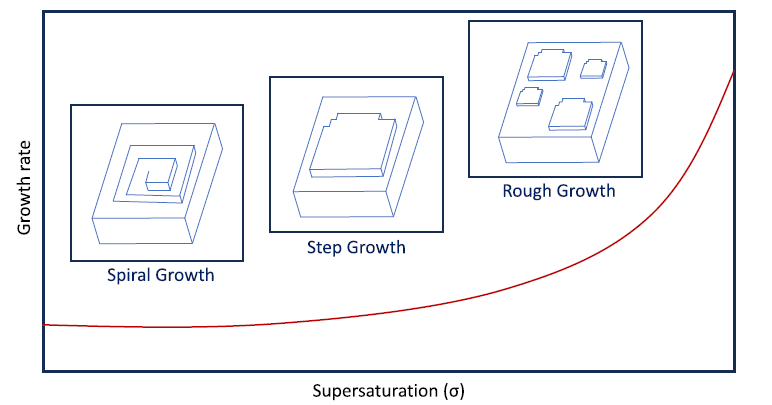
\includegraphics[width=0.6\linewidth]{figures/growth_regimes.png}
    \caption{Diferentes regímenes de crecimiento dependiendo de la sobresaturación.}
    \label{fig:growth_regime}
\end{figure}\\


\subsubsection{Sitios de adsorción del modelo 3D}

El modelo presenta diferentes sitios de adsorción posibles a partir del número de vecinos, en la figura \ref{fig:general_model} se observa un esquema general de cada uno, con sus características individuales que se describen a continuación:\\

\begin{itemize}
    \item \textbf{Adátomo:} Es una unidad aislada que se ha posado sobre una superficie plana y lisa (terraza). Es inestable y representa el punto de partida para el crecimiento "rugoso" a altas sobresaturaciones. Tiene cero vecinos ($n=0$).
    \item \textbf{Borde:} Se define como el final de una capa o escalón en la superficie. Tiene un vecino ($n=1$) y es el sitio clave para el crecimiento por capas o pasos.
    \item \textbf{Codo o Quiebre (Kink):} Es un sitio en un escalón que tiene dos vecinos ($n=2$). Estos sitios son energéticamente muy favorables para la adhesión, ya que forman más enlaces. Se pueden pensar como la esquina interior de una pared de Lego. Un nuevo bloque encaja de forma segura con dos superficies de contacto, haciéndolo mucho más estable que un bloque colocado en medio de una superficie plana. Son esenciales para el crecimiento en espiral a baja sobresaturación.
    \item \textbf{Colgante (Hang):} Un sitio con tres vecinos ($n=3$), característica que le confiere una alta estabilidad y un gran potencial de adsorción para las nuevas unidades.
    \item \textbf{Vacante:} Se puede decir que es un agujero o espacio vacío dentro de una capa de cristal ya formada. Si bien son una característica real de los cristales, es importante notar que el modelo SOS discutido aquí simplifica la realidad al no permitir la formación de vacantes internas, para hacer los cálculos más eficientes. En este modelo se le asigna la cantidad de cuatro vecinos ($n=4$). La interacción entre la sobresaturación y la energía de estos sitios da lugar a diferentes estilos o regímenes de crecimiento.
\end{itemize}\\

\begin{figure}[h!]
    \centering
    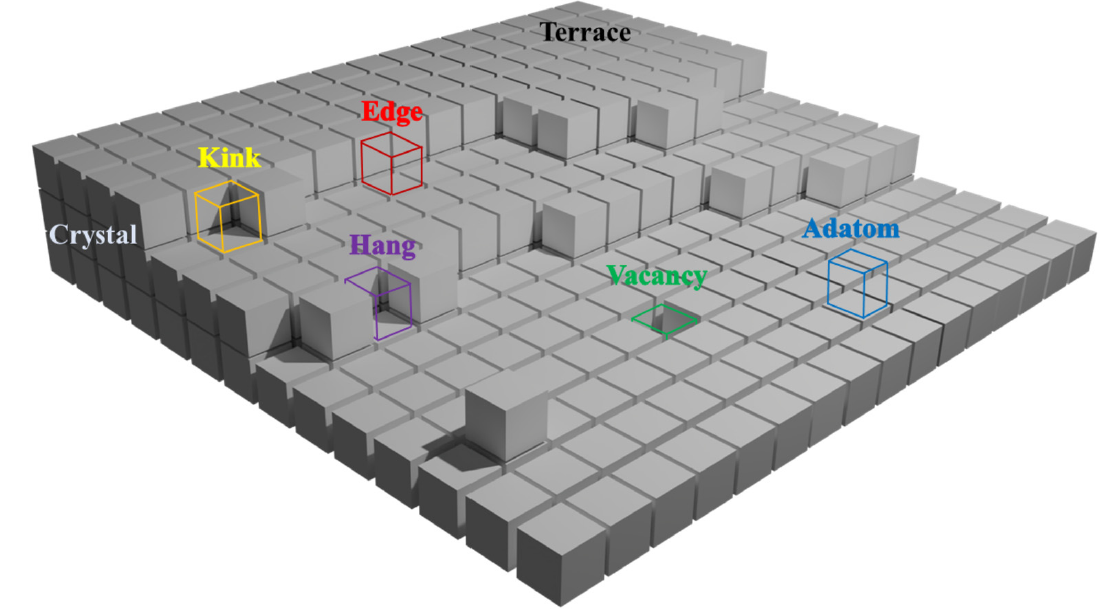
\includegraphics[width=0.6\linewidth]{figures/general_model.png}
    \caption{Visión general de los sitios de adsorción del modelo.}
    \label{fig:general_model}
\end{figure}\\

\subsubsection{Aspectos termodinámicos clave para el modelo 3D}

Hagamos, primero, una descripción de las ecuaciones termodinámicas más importantes implicadas en el modelo. Después, continuamos con las expresiones correspondientes a las tasas de transición.\\

Empecemos por una de las expresiones fundamentales, el potencial químico:\\

\begin{equation}
    \Delta\mu = k_BT\ln\left(\frac{C}{C_{eq}}\right)
    \label{eq:potencial_quimico}
\end{equation}\\

\noindent donde $C$ es la Concentración de soluto, y representa la concentración actual de las unidades de crecimiento en la fase líquida. $C_{eq}$ es la Concentración de equilibrio, y es el valor de saturación a una temperatura específica donde el potencial químico del sólido es igual al de la solución, representando el estado donde el potencial químico del soluto en la fase sólida es igual al de la fase líquida. El cociente entre ambas es la sobresaturación. Si $C > C_{eq}$, entonces $\Delta\mu$ es positivo (en la convención del artículo, indica una disminución de energía potencial al unirse al cristal), lo que proporciona la energía libre necesaria para superar las barreras de adsorción, lo que indica que existe una fuerza termodinámica que favorece la transferencia de unidades de crecimiento hacia el cristal \cite{Nagpal2024}. La ecuación \eqref{eq:potencial_quimico} puede reescribirse en términos de la sobresaturación relativa $\sigma$ como\\

\begin{equation*}
    \sigma = \frac{C}{C_{eq}}-1 ~~~~~\xrightarrow{}~~~~~ \frac{C}{C_{eq}} = \sigma + 1
\end{equation*}\\

\begin{equation}
\Delta\mu = k_BT\ln{\left(\sigma + 1\right)}
\label{eq:mu_sigma}
\end{equation}\\

En adelante, este trabajo usará la ecuación \eqref{eq:mu_sigma} para el potencial químico.\\

Otra relación termodinámica importante a tener en cuenta es la energía libre de Gibbs correspondiente a la creación de una nueva interfaz plana:\\

\begin{equation}
   \Delta G = -N \Delta\mu + \gamma_{edge}A
   \label{eq:gibbs_1}
\end{equation}\\

Esta ecuación describe el cambio global en la energía libre de Gibbs al transferir $N$ unidades de crecimiento a una superficie macroscópicamente plana. El primer término de la ecuación corresponde a la energía libre volumétrica, que siempre es negativo en condiciones de sobresaturación, favoreciendo la estabilidad del cristal. El segundo término representa el trabajo necesario para crear el área de la superficie nueva ($A$), multiplicado por la energía libre superficial específica ($\gamma_{edge}$). Este término es positivo y actúa como una barrera para el crecimiento \cite{Nagpal2024}.\\

Para integrar la termodinámica en el modelo microscópico kMC, Nagpal et al. definen la energía libre asociada a la transferencia de una única unidad de crecimiento (o energía libre por unidad de crecimiento) durante un evento de adsorción, así:\\

\begin{equation}
    \Delta G_{UC} = -\Delta\mu + \gamma_{edge}A_{UC}
    \label{eq:gibbs_2}
\end{equation}\\

En esta ecuación, el término más crítico para la adaptabilidad del modelo es $A_{UC}$. Representa el área nueva expuesta tras la unión de la molécula. Se calcula como $A_{UC} = nA_f$, donde $n$ es el número de vecinos más cercanos del sitio de adsorción y $A_f$ es el área de una cara de la molécula. El producto $\gamma_{edge}A_{UC}$ representa colectivamente la energía de enlace de esa unidad específica en la superficie del cristal.\\

\subsubsection{Tasas de transición del modelo 3D}

La tasa de adsorción en este modelo se define a partir de la $\Delta G_{UC}$, de la siguiente manera:\\

\begin{equation*}
    k_{a_n} = K_0^+\exp{\left(-\frac{\Delta G_{UC}}{k_BT}\right)}
\end{equation*}\\

llegando así, a partir de algunos pasos algebraicos, a la tasa de adsorción\\

\begin{equation}
    k_{a_n} = K_0^+\exp \left(\frac{\Delta\mu}{k_BT} + n_x\frac{\delta_x}{\Delta\mu} + n_y\frac{\delta_y}{\Delta\mu}\right)
    \label{eq:adsorcion}
\end{equation}\\

\noindent donde $(\delta_x,\delta_y)$ son parámetros de energía de unión. Controla el ancho de transición entre regímenes, y es una innovación del trabajo de Nagpal et al. A diferencia de modelos previos donde la adsorción era igual para todos los sitios, aquí la tasa es selectiva. En baja sobresaturación ($\Delta\mu$ pequeña), el término $n\frac{\delta}{\Delta\mu}$ se vuelve muy grande, lo que significa que los sitios con más vecinos tienen una probabilidad de adsorción exponencialmente mayor. A alta sobresaturación, el efecto de $n$ se diluye, permitiendo que la adsorción ocurra en cualquier sitio (lo que corresponde al crecimiento rugoso). En la figura \ref{fig:adosrtion} se observa de manera gráfica los diferentes sitios de adsorción.\\ 

\begin{figure}[h!]
    \centering
    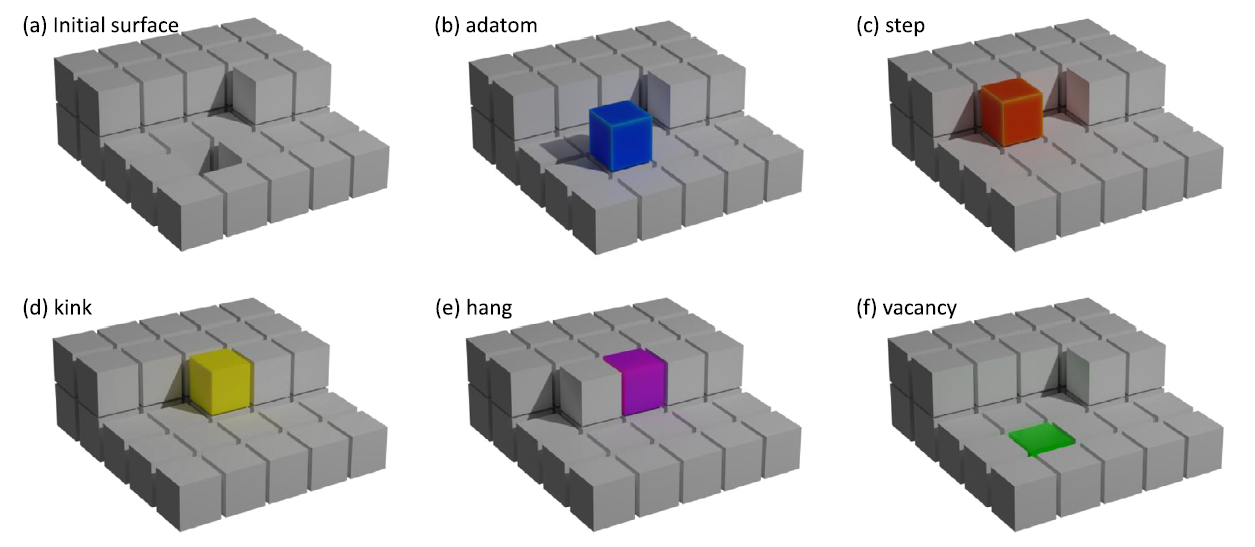
\includegraphics[width=0.65\linewidth]{figures/adsortion.png}
    \caption{Evento de adosrción, con sus diferentes tipos de sitios.}
    \label{fig:adosrtion}
\end{figure}\\


Por su parte, la tasa de desorción viene dada por la siguiente expresión:\\

\begin{equation}
    k_{d_n} = K_0^+\exp \left(\frac{\phi}{k_BT} - n_x\frac{E_{pb_x}}{k_BT} - n_y\frac{E_{pb_y}}{k_BT}\right)
    \label{eq:desorcion}
\end{equation}\\


\noindent donde $\phi$ representa la energía de enlace total, o la energía por unidad de crecimiento en una red completamente ocupada. $E_{pb}$ es la energía necesaria para romper un único enlace entre dos unidades de crecimiento vecinas, es decir, la energía de enlace promedio, por enlace. En este trabajo, la energía $E_{pb}$ se separa en dos direcciones que corresponden a las direcciones bidimensionales de la red inicial. Esto se hace con el fin de modelar la anisotropía de crecimiento y de los diferentes enlaces que forman las hojas 2D de los cristales de HZ, donde $n_x = 0, 1, 2$ y $n_y = 0, 1, 2$.  Así, el término $\phi - n_xE_{pb_x} - n_yE_{pb_y}$ representa la barrera energética que la molécula debe superar para escapar de su sitio actual. Cuando $E_{pb_x} = E_{pb_y}$ entonces se llega al modelo isotrópico y a las ecuaciones de tasas de transición originales de Nagpal et al.\\

Por otro lado, está la tasa de migración o difusión superficial, que permite que una molécula ya adsorbida se mueva a un sitio vecino sin abandonar la superficie:\\

\begin{equation}
    k_{m_n} = K_0^+\exp \left(\frac{\phi}{k_BT} + \frac{E_{pb_x}}{2k_BT} + \frac{E_{pb_y}}{2k_BT} - n_x\frac{E_{pb_x}}{k_BT} - n_y\frac{E_{pb_y}}{k_BT}\right)
    \label{eq:migracion}
\end{equation}\\

El término adicional $\frac{E_{pb}}{2k_BT}$ es la diferencia fundamental con la desorción. Al ser positivo dentro de la exponencial, asegura que la tasa de migración sea siempre mayor que la tasa de desorción. Físicamente, esto significa que es más probable que una molécula migre a un sitio vecino (donde la barrera energética es menor, aproximadamente la mitad de un enlace, $E_{pb}/2)$ que se desprenda totalmente hacia la solución.\\

Finalmente, tenemos la tasa de incorporación:

\begin{equation}
    k_{i_n} = K_{inc}^+\exp \left(n_x\frac{E_{pb_x}}{k_BT} +  n_y\frac{E_{pb_y}}{k_BT}\right)
    \label{eq:desorcion}
\end{equation}\\

Como se observa en la forma de la ecuación, la incorporación está mediada únicamente por los enlaces con los vecinos de la unidad de crecimiento, simulando la incorporación o adhesión total a la superficie del cristal. Esta tasa es añadida en este trabajo y no se encuentra en el modelo implementado por Nagpal et al.\\


\begin{figure}[h!]
    \centering

    \begin{subfigure}{0.5\textwidth}
        \centering
        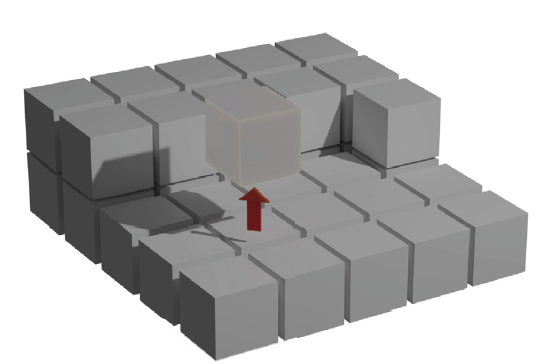
\includegraphics[width=0.55\linewidth]{figures/desortion.png}
        \caption{Evento de desorción.}
    \end{subfigure}
    \hfill
    \begin{subfigure}{0.45\textwidth}
        \centering
        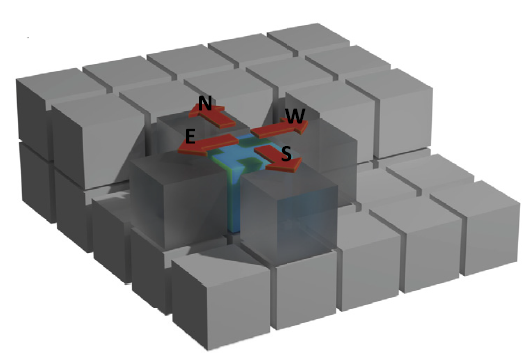
\includegraphics[width=0.55\linewidth]{figures/migration.png}
        \caption{Evento de migración.}
    \end{subfigure}
    \hfill
    \begin{subfigure}{0.5\textwidth}
        \centering
        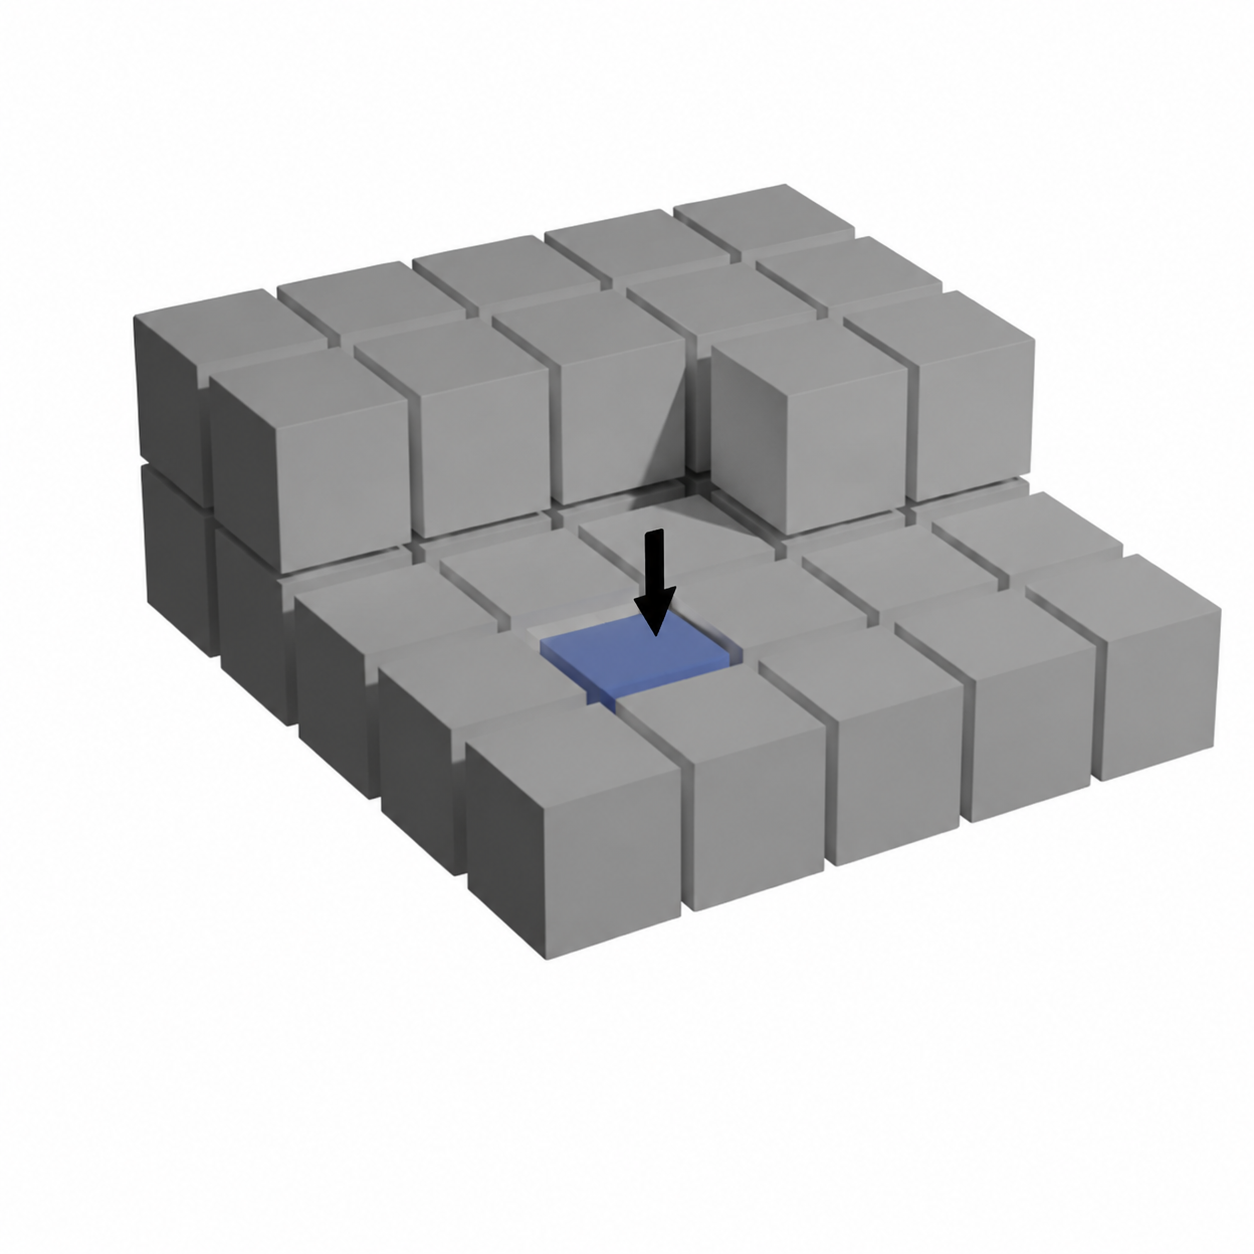
\includegraphics[width=0.55\linewidth]{figures/incorporation.png}
        \caption{Evento de incorporación.}
    \end{subfigure}

    \caption{Visualización gráfica de los eventos del modelo diferentes a la adsorción.}
    \label{fig:eventos}
\end{figure}\\

La figura \ref{fig:eventos} muestra gráficamente el significado de los tres eventos diferentes a la adsorción. Para todas las ecuaciones de las tasas de transición, el término pre-exponencial $K_0^+$  se denomina coeficiente de unión modificado, y es la constante cinética que engloba la frecuencia de colisión de las moléculas con la superficie y factores geométricos de la red.\\

La tasas totales de adsorción, desorción, migración e incorporación se calculan con $M_n$ como la cantidad de sitios reticulares con $n$ vecinos. La tasa total de migración excluye de la sumatoria el sitio de vacancia, pues este no presenta migración:\\

$$W_a = \sum_{n=0}^4M_nk_{a_n}, ~~~~ W_d = \sum_{i=0}^4M_nk_{d_n}, ~~~~ W_m = \sum_{i=0}^3M_nk_{m_n}, ~~~~ W_i = \sum_{n=0}^4M_nk_{i_n}$$\\

Dadas las expresiones para las tasas totales  para los diferentes eventos microscópicos, la tasa total se puede calcular como la suma de estas, de la siguiente manera:\\

\begin{equation}
    W_{tot} = W_a + W_d + W_m + W_i
\end{equation}\\

La probabilidad que decide el evento correspondiente se define como $P_j = W_j / W_{tot}$ y las condiciones para ejecutar el evento se definen en la tabla 1. La tabla 2 representa las condiciones de selección de eventos para los cuatro eventos en función de sus vecinos más cercanos. Para la migración, las clases de sitios de la red se eligen en función de una dirección aleatoria, ya que una unidad de crecimiento no puede migrar a una capa superior. Por lo tanto, primero se elige una dirección al azar y luego se comprueba si la migración es factible. Hay un incremento de tiempo correspondiente independientemente de si el evento tiene éxito o no. Para el trabjo de Nagpal et al., un sitio de migración disponible se refiere al sitio vecino más cercano de menor altura que el sitio de la red actual donde ocurre el evento de migración.\\

\begin{table}[h!]
\centering
\begin{minipage}{0.78\textwidth}
\raggedright
\textbf{Tabla 1}\\
Condiciones de probabilidad para seleccionar un evento kMC.
\vspace{0.6em}

\centering
\renewcommand{\arraystretch}{1.25}
\setlength{\tabcolsep}{18pt}
\begin{tabular}{@{}>{\centering\arraybackslash}p{0.48\textwidth} >{\centering\arraybackslash}p{0.30\textwidth}@{}}
\hline
\textbf{Condiciones de probabilidad} & \textbf{Evento ejecutado} \\
\hline
$0<\zeta\leq P_a$ & Adsorción \\
$P_a<\zeta\leq P_a+P_d$ & Desorción \\
$P_a+P_d<\zeta\leq P_a+P_d+P_m$ & Migración \\
$P_a+P_d+P_m<\zeta\leq 1$ & Incorporación \\
\hline
\label{tab:table1}
\end{tabular}
\end{minipage}
\end{table}

\vspace{1.4em}

\begin{table}[h!]
\centering
\begin{minipage}{0.88\textwidth}
\raggedright
\textbf{Tabla 2}\\
Condiciones de probabilidad para seleccionar el caso de hematina $n$ con un evento definido como $j=1$ (adsorción), $2$ (desorción), $3$ (migración), $4$ (incorporación).
\vspace{0.6em}

\centering
\renewcommand{\arraystretch}{1.25}
\setlength{\tabcolsep}{16pt}
\begin{tabular}{@{}>{\centering\arraybackslash}p{0.70\textwidth} >{\centering\arraybackslash}p{0.18\textwidth}@{}}
\hline
\textbf{Condiciones de probabilidad} & \textbf{Número de vecinos} \\
\hline
$\displaystyle 0<\zeta_j \leq \frac{r_j^{(0)}}{\sum_{n=0}^{4} r_j^{(n)}}$ & Cero \\
$\displaystyle \frac{r_j^{(0)}}{\sum_{n=0}^{4} r_j^{(n)}} < \zeta_j \leq \frac{\sum_{n=0}^{1} r_j^{(n)}}{\sum_{n=0}^{4} r_j^{(n)}}$ & Uno \\
$\displaystyle \frac{\sum_{n=0}^{1} r_j^{(n)}}{\sum_{n=0}^{4} r_j^{(n)}} < \zeta_j \leq \frac{\sum_{n=0}^{2} r_j^{(n)}}{\sum_{n=0}^{4} r_j^{(n)}}$ & Dos \\
$\displaystyle \frac{\sum_{n=0}^{2} r_j^{(n)}}{\sum_{n=0}^{4} r_j^{(n)}} < \zeta_j \leq \frac{\sum_{n=0}^{3} r_j^{(n)}}{\sum_{n=0}^{4} r_j^{(n)}}$ & Tres \\
$\displaystyle \frac{\sum_{n=0}^{3} r_j^{(n)}}{\sum_{n=0}^{4} r_j^{(n)}} < \zeta_j \leq 1$ & Cuatro \\
\hline
\end{tabular}
\end{minipage}
\end{table}\\


Los pasos seguidos para la simulación se basan en el algoritmo BKL ya descrito anteriormente en la sección \ref{sec:kMC_theory} y cuyo diagrama de flujo se esquematiza a detalle en la figura \ref{fig:diagram}. \\

\begin{figure}[h!]
    \centering
    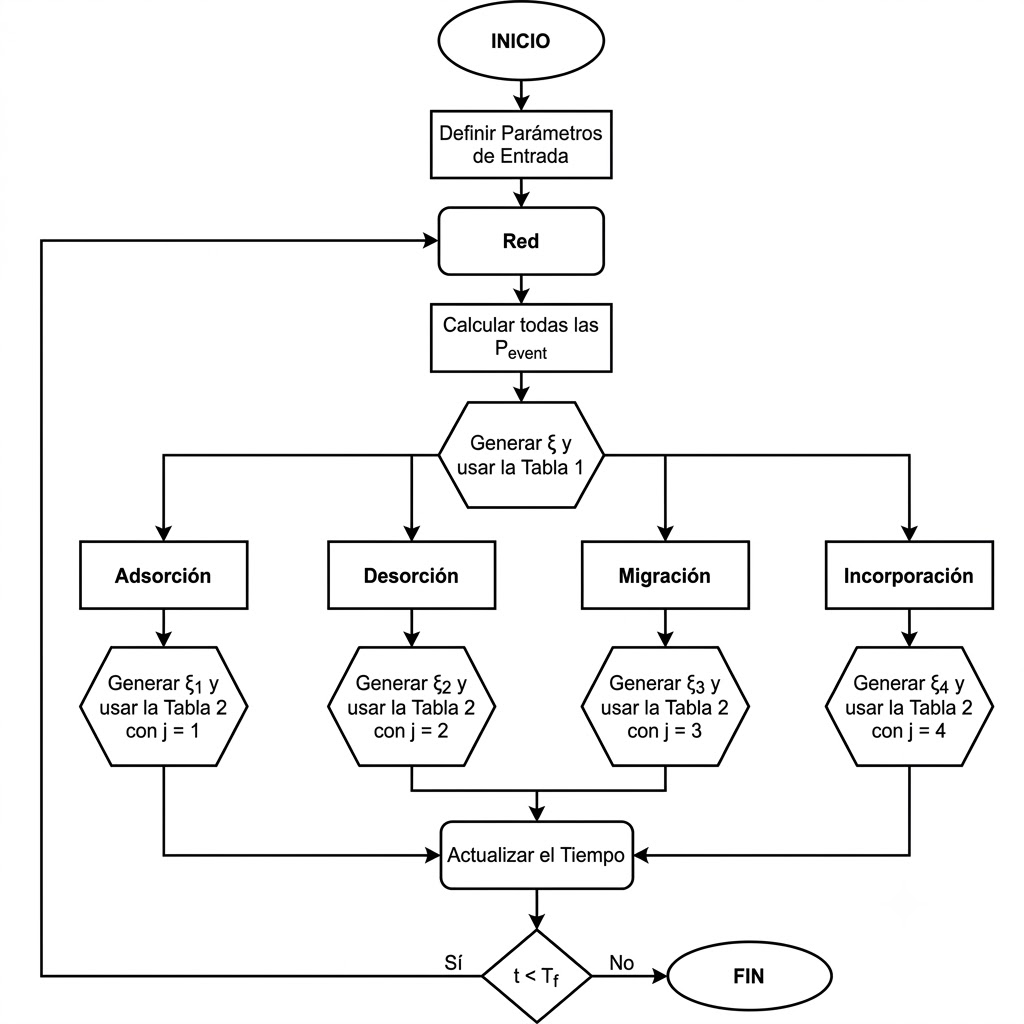
\includegraphics[width=0.5\linewidth]{figures/diagrama.png}
    \caption{Diagrama de flujo del algoritmo kMC adaptado para simular el crecimiento de cristales en diversos regímenes de crecimiento.}
    \label{fig:diagram}
\end{figure}\\

\section{Cálculo \textit{ab initio} de los parámetros kMC}\label{sec:abini}

Como ya se discutió en la sección \ref{sec:GU_cry}, en este trabajo se toma como referencia la estructura reportada por Pagola et al., y trabajos modernos como los de Becker et al. \cite{PagolaSilvina2000, becker2016bhematin}. Sin embargo, así como en Klois et al. \cite{Klonis2010}, en el trabajo de Ma et al. \cite{nonclassical2025ma} se propone que la unidad de crecimiento más estable corresponde a un arreglo por apilamiento $\pi\text{-}\pi$ (ver Figura \ref{fig:comparacion_hemo}). Con el propósito de seguir este modelo, se adaptó la estructura original de Becker empleando sus coordenadas cristalográficas para construir el dímero de apilamiento $\pi\text{-}\pi$.\\

Para obtener la estructura final empleada en los cálculos energéticos, se sometió al dímero de apilamiento $\pi\text{-}\pi$ a un proceso de relajación geométrica. Para ello, se utilizó el software ASE (Atomic Simulation Environment) en combinación con el calculador MACE, un potencial interatómico basado en Machine Learning (MLIP) \cite{batatia2023mace}.\\

\subsection{MLIPs: MACE}
\label{subsec:metodo_mace}

El estudio de sistemas moleculares complejos en física del estado sólido y química computacional requiere describir con alta precisión las interacciones atómicas. Así es posible determinar estructuras de mínima energía y trayectorias dinámicas. Tradicionalmente, niveles altos de precisión se alcanzan mediante métodos \textit{ab initio} basados en la teoría del funcional de densidad (DFT). Sin embargo, el costo computacional del DFT escala de forma cúbica o superior con respecto al número de electrones del sistema ($\mathcal{O}(N^3)$) \cite{capelle2006birds}. Esto limita en la práctica la exploración de sistemas de gran tamaño o simulaciones de dinámica molecular en escalas de tiempo macroscópicas.\\

Como alternativa para superar este cuello de botella computacional, en los últimos años han emergido los potenciales interatómicos basados en Machine Learning (MLIPs, por sus siglas en inglés). Los MLIPs actúan como interpoladores de alta fidelidad, se entrenan a partir de un conjunto de datos previos calculados con metodologías \textit{ab initio} (como DFT) para aprender la superficie de energía potencial del sistema. Una vez entrenado, el modelo es capaz de predecir energías y fuerzas atómicas con una precisión cercana a la de los métodos cuánticos primarios, pero con un costo computacional drásticamente menor, permitiendo un escalamiento lineal $\mathcal{O}(N)$ comparable al de los campos de fuerza clásicos \cite{batatia2023mace}.\\

Dentro de los MLIPs de última generación, MACE (Multi-Layer Atomic Cluster Expansion) destaca por el uso de redes neuronales de paso de mensajes equivariantes (MPNN) \cite{batatia2023mace, batatia2026macepolar}. A diferencia de los potenciales invariantes tradicionales, MACE preserva explícitamente la simetría rotacional y traslacional del espacio tridimensional mediante el uso de armónicos esféricos para describir los entornos atómicos. Esto le permite capturar interacciones físicas de largo alcance y correlaciones de muchos cuerpos (\textit{higher-order many-body interactions}) con un número significativamente menor de parámetros y datos de entrenamiento.\\

En este trabajo, MACE en su modelo \textit{polar}, se establece como el motor de cálculo fundamental. Este modelo permite el calculo de energías de grandes sistemas como lo es la UC de hemozina (con 148 átomos por cada UC) incorporando interacciones electrostáticas con un bajo coste computacional y una alta precisión \cite{batatia2026macepolar}. El modelo \textit{polar} en sus versiones \textsc{medium} y \textsc{large} fue entrenado empleando la base de datos OMol25 \cite{ batatia2026macepolar,omol2025}, esta base de datos corresponde a cálculos realizados con el funcional $\omega\text{B97M-V}$ el cual captura interacciones electrostáticas de largo alcance \cite{mardirossian2016wb97m}.\\

La arquitectura de MACE-\textit{polar} se divide en dos componentes principales: la predicción de energía en entornos locales ($E_{\text{local}}$) mediante MACE como MPNN \cite{batatia2023mace} y la predicción de la energía no local y electrostática ($E_{\text{non-local}} + E_{\text{electrostatic}}$) mediante una construcción de la densidad de espín-carga en un modelo de expansión multipolar \cite{batatia2026macepolar}. Ambos componentes son procesos basados en Machine Learning: el primero predice la energía del estado base de una configuración atómica al suponer los sistemas atómicos como grafos cuyos nodos vecinos pueden interactuar a través de un proceso denominado como construcción e intercambio de mensaje como se ve en la figura \ref{subfig:diagrama_mace_local}. Esta construcción de mensaje se produce como una expansión en una base radial aprendida (empleando las funciones de Bessel) y los armónicos esféricos. Los coeficientes de la expansión mezclan las características de cada nodo que participa del intercambio. A través de un proceso de lectura en el cual se emplea un perceptrón multicapa (MLP) cada configuración atómica predice una energía local \cite{batatia2023mace}. El segundo componente predice la densidad de espín-carga de la configuración atómica mediante una expansión multipolar que emplea orbitales de tipo Gaussiano, los coeficientes de la expansión se predicen mediante un MLP de las características de cada nodo. Estos coeficientes se emplean para la predicción de las energías no locales y electrostáticas como se muestra en la figura \ref{subfig:diagrama_mace_polar_lr}, la primera a través de una sucesión de MLP sobre las características de los nodos de la configuración y la segunda integrando la energía de Hartree y el potencial externo aplicado \cite{batatia2026macepolar}.\\


\begin{figure}[h!]
    \centering
    % =========================================================================
    % SUBFIGURE A: MACE (Message Passing)
    % =========================================================================
    \begin{subfigure}[b]{0.49\textwidth}
        \centering
        \begin{tikzpicture}[
            scale=0.65,                        % Escala el lienzo para el subplot izquierdo
            every node/.style={scale=0.65},     % Escala el texto de forma uniforme
            node distance=0.9cm,
            auto,
            block/.style={
                rectangle, 
                draw=black, 
                thick,
                fill=gray!10, 
                text width=7.0cm,              % Ancho adaptado para la columna izquierda
                text centered, 
                rounded corners, 
                minimum height=1.2cm,
                font=\small
            },
            line/.style={
                draw, 
                -latex, 
                thick
            }
        ]
            % --- NODOS MACE ---
            \node [block, fill=blue!5] (input) {
                \textbf{Entrada: Configuración Atómica} \\ 
                Coordenadas cartesianas $\vec{r}_i$ y números atómicos $Z_i$ para la conformación de $\vec{\sigma}_i$
            };
            
            \node [block, below=of input] (embedding) {
                \textbf{1. Bloque de Embedding } \\ 
                \textbf{Atómico:} $Z_i \rightarrow h_i^{(0)}$ \\ \textbf{Geométrico:} Radial y Angular $Y_l^m(\hat{r}_{ij})$
            };
            
            \node [block, below=of embedding] (messages) {
                \textbf{2. Construcción de Mensajes} \\ 
                Combinación densa de bases para formar los coeficientes $B_{i, \eta \nu kLM}$ del mensaje $m_i^{(t)}$
            };
            
            \node [block, below=of messages] (update) {
                \textbf{3. Actualización de Estados} \\ 
                Actualización del embedding invariante: $h_i^{(t+1)} = W(m_i^{(t)},h_i^{(t)})$
            };
            
            \node [block, below=of update] (readout) {
                \textbf{4. Lectura Local} \\ 
                Mapeo via MLP para predecir la energía del sitio local: $E_i = \mathcal{R}(h_i^{(0)},\dots,h_i^{(T)})$
            };
            
            \node [block, below=of readout, fill=green!5] (output) {
                \textbf{Salida: Energía Total MACE} \\ 
                Predicción por suma directa: $E_{\text{local}} = \sum_{i} E_i$
            };
            
            % --- ENLACES MACE ---
            \path [line] (input) -- (embedding);
            \path [line] (embedding) -- (messages);
            \path [line] (update) -- (readout);
            \path [line] (readout) -- (output);
    
            \path [line] (messages.west) to[out=180, in=180, looseness=1.0] node[left, pos=0.5, font=\scriptsize] {Iteración $t$} (update.west);
            \path [line] (update.east) to[out=0, in=0, looseness=1.0] (messages.east);
        \end{tikzpicture}
        \caption{Algoritmo MACE (Interacciones locales).}
        \label{subfig:diagrama_mace_local}
    \end{subfigure}
    \hfill % Fuerza la separación horizontal máxima entre ambos subplots
    %=========================================================================
    % SUBFIGURE B: MACE-POLAR (Long-Range / Electrostatic)
    % =========================================================================
    \begin{subfigure}[b]{0.49\textwidth}
        \centering
        \begin{tikzpicture}[
            scale=0.65,                        % Escala el lienzo para el subplot derecho
            every node/.style={scale=0.64},     % Escala el texto de forma uniforme
            node distance=0.9cm,
            auto,
            block/.style={
                rectangle, 
                draw=black, 
                thick,
                fill=gray!10, 
                text width=7.0cm,              % Ancho adaptado para la columna derecha
                text centered, 
                rounded corners, 
                minimum height=1.2cm,
                font=\small
            },
            line/.style={
                draw, 
                -latex, 
                thick
            }
        ]
            % --- NODOS MACE-POLAR ---
            \node [block, fill=blue!5] (input_p) {
                \textbf{Entrada: Restricciones Globales} \\ 
                Posiciones Atómicas, Carga Total $Q$ y Espín Total $S$
            };
            
            \node [block, below=of input_p] (init_p) {
                \textbf{1. Inicialización de Multipolos} \\ 
                Predicción de multipolos iniciales $\tilde{p}_{i,lm}^{(0)}$ y funciones de Fukui $f_i^{(0)}$ desde MACE
            };
            
            \node [block, below=of init_p] (poisson_p) {
                \textbf{2. Solución de Poisson Global} \\ 
                Construcción de la densidad $\rho(r)$ y convolución con el núcleo de Coulomb para obtener $v(r)$
            };
            
            \node [block, below=of poisson_p] (induction_p) {
                \textbf{3. Inducción y Equilibrio} \\ 
                Refinamiento de multipolos $p_{i,lm}^{(u)}$ + Normalización de Fukui para conservar $Q$ y $S$
            };
            
            \node [block, below=of induction_p] (energy_p) {
                \textbf{4. Cálculos Energéticos} \\ 
                \textbf{Electrostática:} $E = \frac{1}{2} \int \rho v$ \\ \textbf{No-Local:} $E = \text{MLP}(\vec{h}^{(T)})$
            };
            
            \node [block, below=of energy_p, fill=green!5] (output_p) {
                \textbf{Salida: Energía No-Local Total} \\ 
                $E_{\text{LR}} = E_{\text{electrostatic}} + E_{\text{non-local}}$
            };
            
            % --- ENLACES MACE-POLAR ---
            \path [line] (input_p) -- (init_p);
            \path [line] (init_p) -- (poisson_p);
            \path [line] (induction_p) -- (energy_p);
            \path [line] (energy_p) -- (output_p);
            
            \path [line] (poisson_p.west) to[out=180, in=180, looseness=1.0]  (induction_p.west);
            \path [line] (induction_p.east) to[out=0, in=0, looseness=1.0] node[right, pos=0.5, font=\scriptsize] {Inducción $u$}(poisson_p.east);
        \end{tikzpicture}
        \caption{MACE-Polar (Efectos de largo alcance).}
        \label{subfig:diagrama_mace_polar_lr}
    \end{subfigure}

    \caption{Arquitectura integrada de MACE y MACE-Polar para el cálculo de propiedades moleculares.}
    \label{fig:arquitectura_mace_completa}
\end{figure}\\

\subsection{Relajación de la Estructura}

Para la determinación de la estructura cristalina óptima, se tomó como configuración inicial el dímero con apilamiento $\pi\text{-}\pi$ obtenido a partir de la UC reportada por Becker et al. \cite{becker2016bhematin}, ilustrada en la Figura \ref{subfig:pipi}. Los parámetros de red experimentales de dicha referencia se utilizaron para construir la celda unitaria inicial, aplicando condiciones periódicas de frontera (PBC) en las tres dimensiones. Las interacciones interatómicas se modelaron empleando el modelo \textit{polar-1-l} de MACE.\\

El proceso de relajación estructural se llevó a cabo en dos etapas consecutivas utilizando el entorno ASE. En la primera etapa, se realizó una optimización geométrica exclusiva de la celda manteniendo las posiciones atómicas fijas en coordenadas fraccionarias; para ello, se empleó el formalismo de deformación homogénea mediante la herramienta \texttt{StrainFilter} acoplada al algoritmo Cuasi-Newton de memoria limitada L-BFGS, utilizando un criterio de convergencia en las fuerzas de $F_{\text{max}} = 0.05$ \text{ eV/\AA}. En la segunda etapa, se procedió con una relajación conjunta y acoplada de las coordenadas atómicas y los vectores de la celda (relajación de celda variable). Esta fase se ejecutó mediante el algoritmo \texttt{FrechetCellFilter} en el espacio exponencial y el optimizador L-BFGS, bajo un criterio de convergencia más estricto de $F_{\text{max}} = 0.01$ \text{ eV/\AA}.\\

Como resultado de este protocolo de optimización, se determinaron los parámetros de red calculados para el estado base del cristal: $a = 16.218$ \text{\AA}, $b = 24.214$ \text{\AA}, $c = 7.758$ \text{\AA}, $\alpha = 135.440^\circ$, $\beta = 120.054^\circ$ y $\gamma = 37.008^\circ$, para una comparación con los parámetros iniciales ver la tabla \ref{tab:parametros_red}.\\

% =========================================================================
% SECCIÓN OPCIONAL: Sugerencia de tabla para comparar con el experimento
% =========================================================================
\begin{table}[h!]
\centering
\caption{Comparación de los parámetros de red determinados mediante el campo de fuerza por Becker et al. \cite{becker2016bhematin} frente a los valores optimizados mediante el potencial MACE (\textit{polar-1-l}).}
\label{tab:parametros_red}
\begin{tabular}{lcc}
\toprule
\textbf{Parámetro} & \textbf{Previo \cite{becker2016bhematin}} & \textbf{Optimizado (Este trabajo)} \\
\midrule
$a$ (\AA)       & $16.636$ & $16.218$ \\
$b$ (\AA)       & $24.846$ & $24.214$ \\
$c$ (\AA)       & $7.990$ & $7.758$  \\
$\alpha$ ($^\circ$) & $135.205$ & $135.440$ \\
$\beta$ ($^\circ$)  & $119.553$ & $120.054$ \\
$\gamma$ ($^\circ$) & $36.874$ & $37.008$  \\
\bottomrule
\end{tabular}
\end{table}

\subsection{Cálculos de Energía de Enlace ($E_{\text{pb}}$)}
\label{subsec:calculos_epb}

Para la determinación de las energías de enlace ($E_{\text{pb}}$), se tomó como estado de referencia la UC relajada bajo condiciones periódicas de frontera (PBC). Debido a la naturaleza intrínseca del cálculo de interacciones aisladas, es necesario desactivar las PBC y realizar una re-optimización geométrica en el vacío.\\ 

Con el propósito de evitar artefactos estructurales artificiales en el vacío, tales como el colapso de los grupos carboxilo terminales que originalmente se coordinan con los centros de hierro de las UC adyacentes, se procedió a saturar los átomos de oxígeno externos mediante la adición de átomos de hidrógeno (ver la figura \ref{fig:H-extra}). Físicamente, se puede aproximar a la presencia de una solución.\\

\begin{figure}[h!]
    \centering
    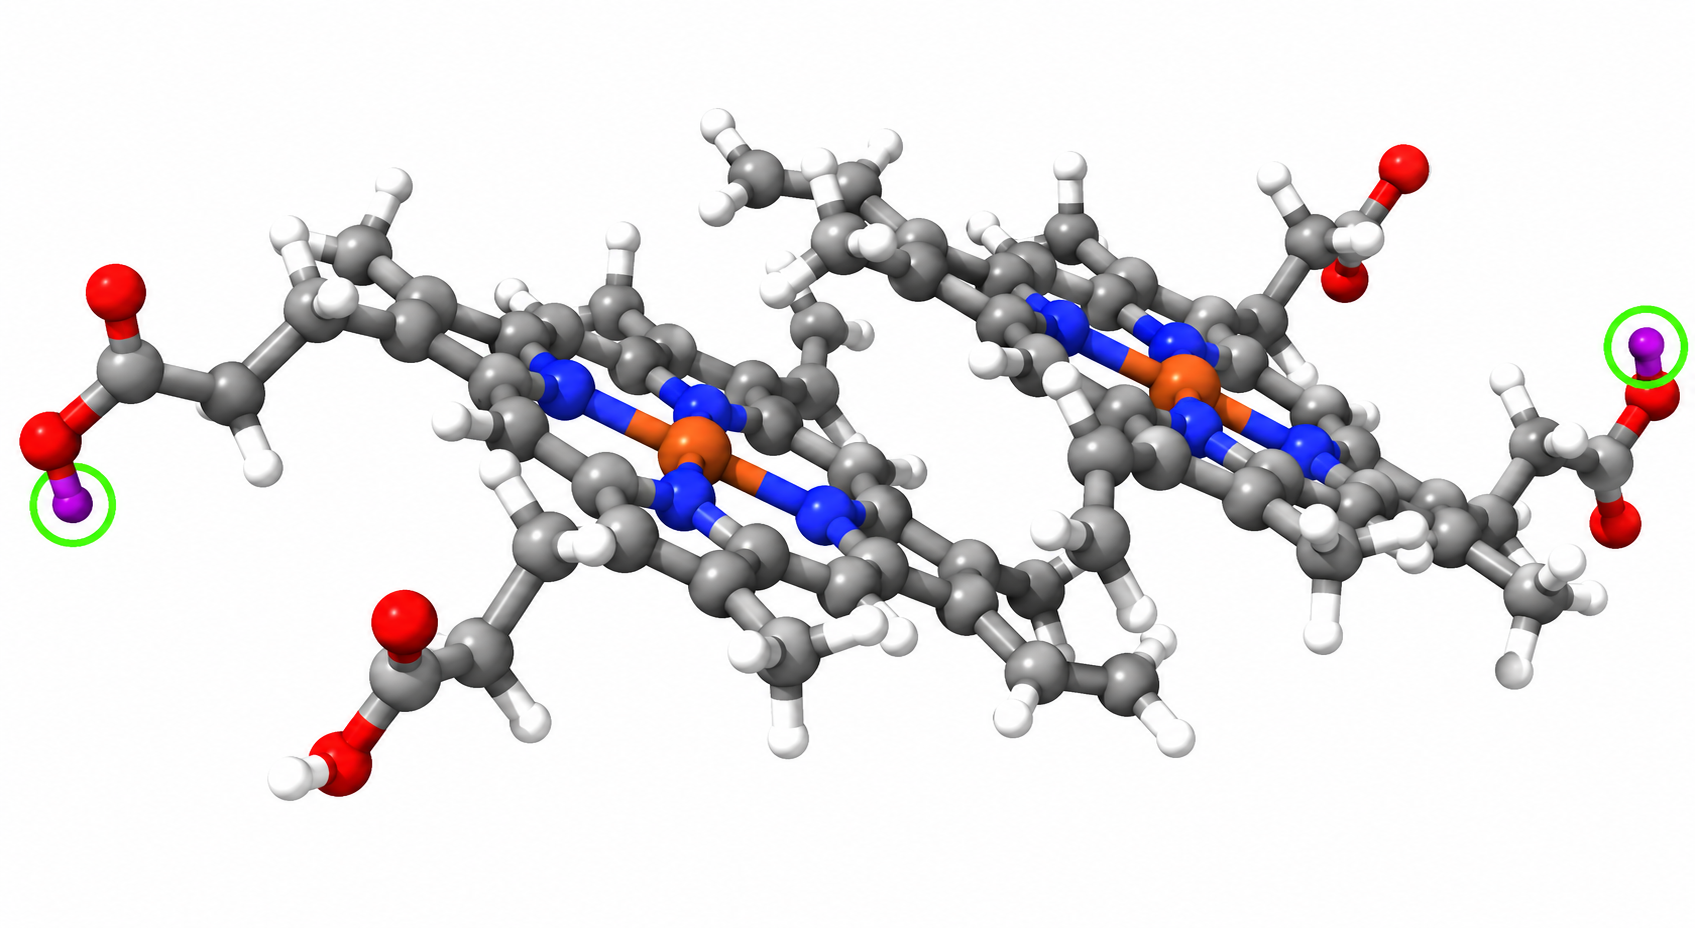
\includegraphics[width=0.8\linewidth]{figures/H_extra_c.png}
    \caption{Estructura con adición de Hidrógenos para la estabilización de la geometría.}
    \label{fig:H-extra}
\end{figure}\\

El protocolo de relajación de las UC modificadas se ejecutó en dos etapas sucesivas mediante el algoritmo LBFGS:\\

\begin{enumerate}
    \item \textbf{Optimización parcial:} Se mantuvieron fijos todos los átomos de la UC original, permitiendo la libre movilidad únicamente de los hidrógenos añadidos para optimizar las distancias de enlace de los grupos hidroxilo.
    \item \textbf{Optimización global:} Se liberaron todos los grados de libertad del sistema hasta alcanzar la convergencia geométrica total.
\end{enumerate}\\

Para aislar y contrarrestar la contribución energética de los hidrógenos extra en el balance termodinámico, se optimizó de manera independiente una molécula de $\text{H}_2$ en el vacío bajo el mismo nivel de teoría. Así, para la dirección del enlace $\mu\text{-propionato}$, donde se remueven los hidrógenos correspondientes para evaluar la coordinación metal-ligando, la energía se computa como:\\

\begin{equation*}
    E_{\mu\text{-Pr}} = E_{\text{dim}} + E_{\text{H}_2} - 2E_{\text{UC}}
\end{equation*}\\

Mientras que para las componentes restantes, donde no se requiere la remoción de los agentes de saturación, la energía de interacción se define directamente mediante la diferencia:\\

\begin{equation*}
    E_{\text{pb}} = E_{\text{dim}} - 2E_{\text{UC}}
\end{equation*}\\

Los resultados energéticos obtenidos a través del calculador MACE, junto con las energías de interacción molecular para cada orientación cristalográfica y sus respectivos promedios de par, se consolidan en la tabla \ref{tab:energias_hemozoin}.\\

\begin{table}[h!]
    \centering
    \caption{Energías totales calculadas de enlace $E_{\text{pb}}$ determinadas con MACE}
    \label{tab:energias_hemozoin}
    \small
    \begin{tabular}{lc}
        \hline
        \textbf{Configuración / Parámetro} & \textbf{Energía (eV)} \\ \hline
        Energía de un monómero aislado relajado ($E_{\text{UC}}$) & $-168\,634.0454$ \\ [1ex]
        \textbf{Energías de Enlace ($E_{\text{pb}}$)} & \\
        \quad Dirección $\mu$-propionato & $-0.7609$ \\
        \quad Dirección Enlace de Hidrógeno (H-Bond) & $-0.7420$ \\
        \quad Dirección P-P & $-2.1994$ \\ [1ex]
        \textbf{Promedios de Pares Intermoleculares} & \\
        \quad Promedio $\mu$-propionato \,+\, H-Bond & $-0.7514$ \\
        \quad Promedio $\mu$-propionato \,+\, P-P & $-1.4801$ \\
        \quad Promedio H-Bond \,+\, P-P & $-1.4707$ \\ [1ex]
        \hline
        \textbf{PROMEDIO TOTAL DE ENLACE} & $\mathbf{-1.2341}$ \\ \hline
    \end{tabular}
    \label{table:MACE}
\end{table}\\

\chapter{Resultados y discusión}

\section{Validación de los modelos implementados}

El primer paso para garantizar la trazabilidad de los resultados obtenidos en este trabajo, fue reproducir algunos resultados del estudio de Nagpal et al. para el modelo 3D. En este caso, se reprodujo un observable muy utilizado en el crecimiento superficial de cristales y en las implementaciones kMC: la tasa de crecimiento superficial en términos de la sobresaturación (ver Figura \ref{subfig:GR}), que sirve para analizar la rapidez con la que crecen las capas superficiales del cristal. En el trabajo de Nagpal et al., se hace un análisis por caras para cristales de Lizosima, con unos parámetros del modelo específicos, que fueron calibrados por \textit{search grid}. Por otro lado, se reprodujo la probabilidad por sitios de adsorción, en términos de la sobresaturación (ver Figura \ref{subfig:PvsSite}). Este último, sirve para analizar los regímenes de crecimiento a partir de la coordinación local de la red.\\

Una vez realizada la reproducción de estos resultados, se tiene plena confianza en el funcionamiento del código implementado, y se garantiza que puede ser usado para adaptarse al contexto del crecimiento superficial de cristales de HZ. Mientras tanto, para el modelo 2D, al ser una versión simplificada y un paso previo para la construcción del modelo 3D, se consideró que no fue necesaria una validación de este tipo.\\


\begin{figure}[h!]
    \centering

    \begin{subfigure}[t]{0.4\textwidth}
        \centering
        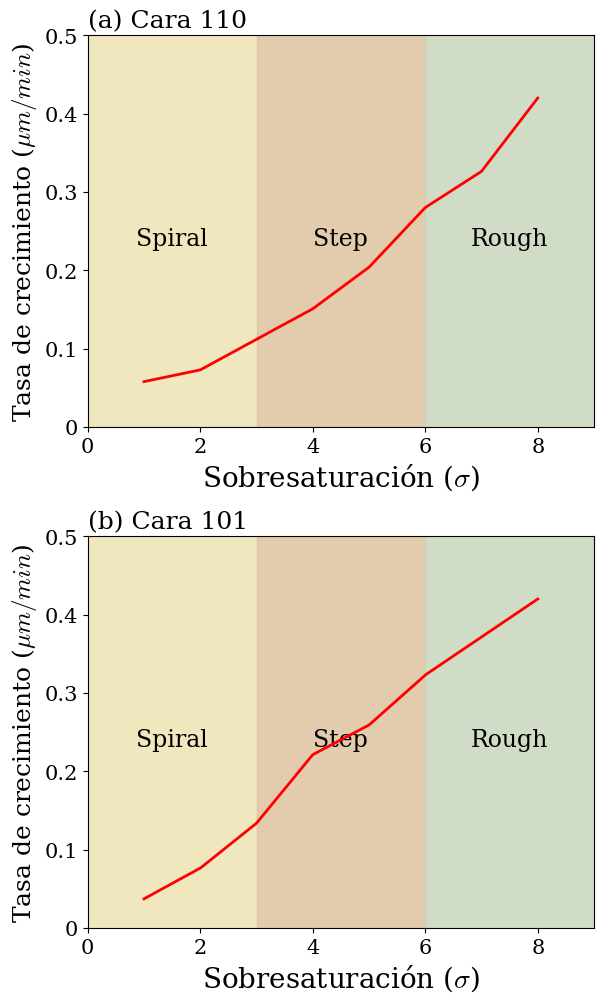
\includegraphics[width=\linewidth]{results/growth_rate_val.png}
        \caption{Índice o tasa de crecimiento para las caras [110] y [101] de cristal de Lizosima, en términos de la sobresaturación.}
        \label{subfig:GR}
    \end{subfigure}
    \hfill
    \begin{subfigure}[t]{0.45\textwidth}
        \centering
        \raisebox{2.5cm}[0pt][0pt]{%
            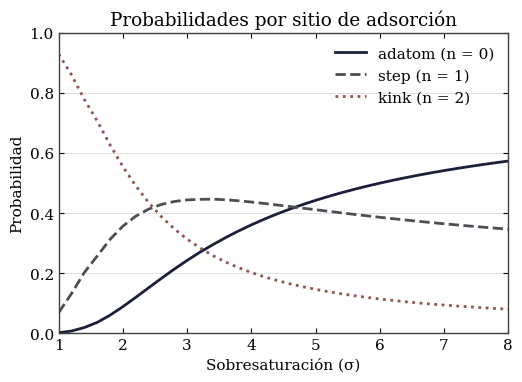
\includegraphics[width=\linewidth]{results/PvsSite.png}%
        }
        \caption{Probabilidades de adsorción, por sitio de adsorción, en relación a la sobresaturación.}
        \label{subfig:PvsSite}
    \end{subfigure}

    \caption{Validación de la implementación del modelo 3D isotrópico, a partir de la reproducción de los resultados para Lizosima en Nagpal et al.}
    \label{fig:validacion}
\end{figure}


\section{Resultados para el modelo 2D}

La ejecución de las simulaciones para el modelo 2D se realizaron con un tamaño de $80\times80$ para la red de sitios de adsorción. El intervalo de tiempo simulado fue de $[0, 240]$ minutos.\\

Con todo esto, se obtuvo la morfología de crecimiento superficial a lo largo del tiempo (figura \ref{fig:seis_imagenes_2x3}), y la cinética de crecimiento superficial (figura \ref{fig:cinetica2d}) que a su vez se compara con los ajustes de los tres modelos de cinética de crecimiento. En la tabla \ref{table:kMC2d} se observa la comparación de los valores de bondad de ajuste de estos tres modelos, con la reproducción de la cinética de crecimiento mediante kMC para el modelo 2D, observando un ajuste satisfactorio y que mejora el modelo de Avrami, y se acerca a los ajustes de segundo orden y de Pasternack.


\begin{figure}[h!]
    \centering
    
    \begin{subfigure}[t]{0.25\textwidth}
        \centering
        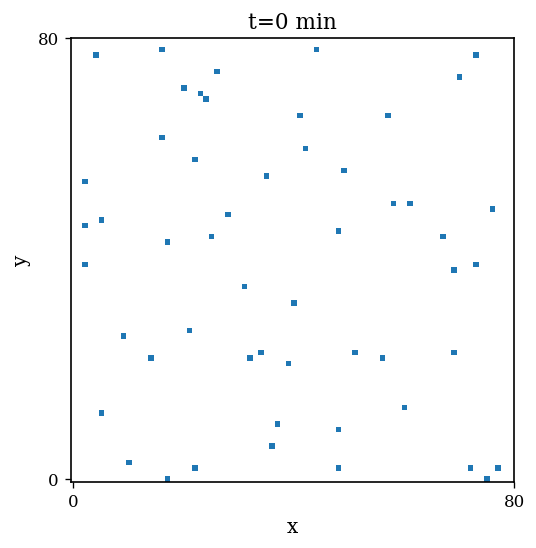
\includegraphics[width=\linewidth]{results/2d_1_snap.png}
        %\caption{Imagen 1}
    \end{subfigure}\hfill
    \begin{subfigure}[t]{0.25\textwidth}
        \centering
        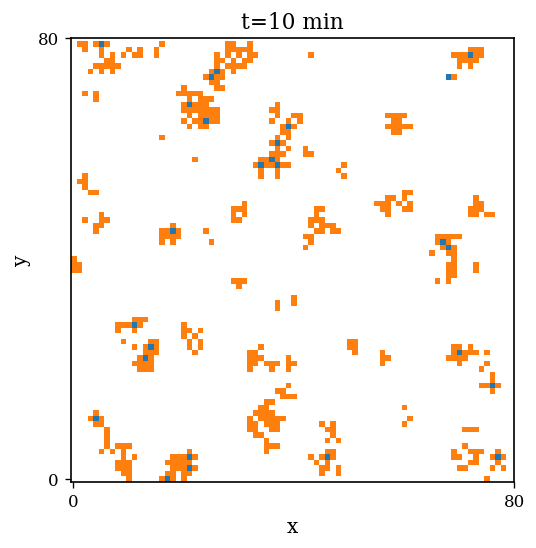
\includegraphics[width=\linewidth]{results/2d_2_snap.png}
        %\caption{Imagen 2}
    \end{subfigure}\hfill
    \begin{subfigure}[t]{0.25\textwidth}
        \centering
        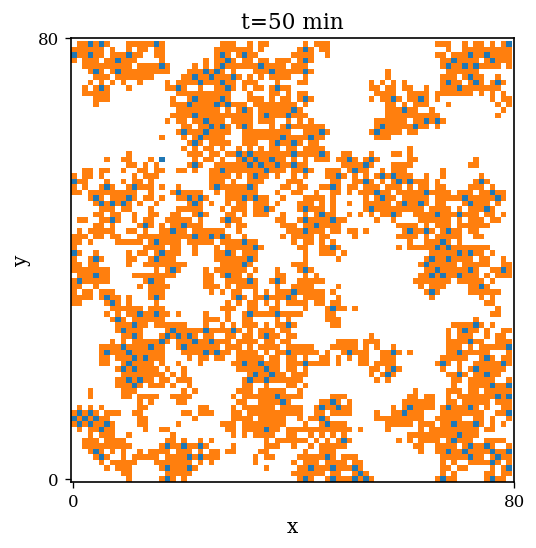
\includegraphics[width=\linewidth]{results/2d_3_snap.png}
        %\caption{Imagen 3}
    \end{subfigure}

    \vspace{0.3cm}

    \begin{subfigure}[t]{0.25\textwidth}
        \centering
        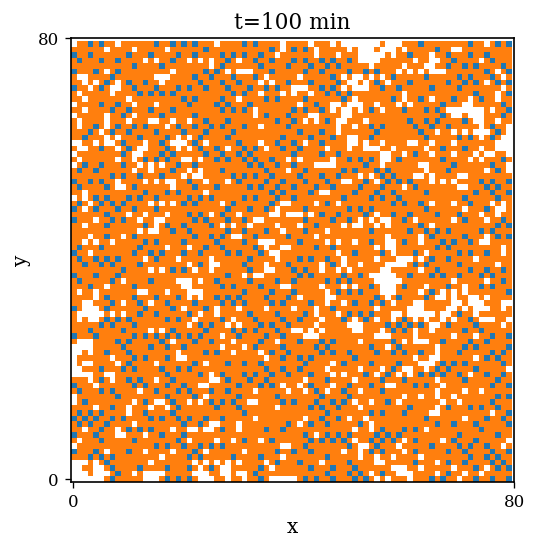
\includegraphics[width=\linewidth]{results/2d_4_snap.png}
        %\caption{Imagen 4}
    \end{subfigure}\hfill
    \begin{subfigure}[t]{0.25\textwidth}
        \centering
        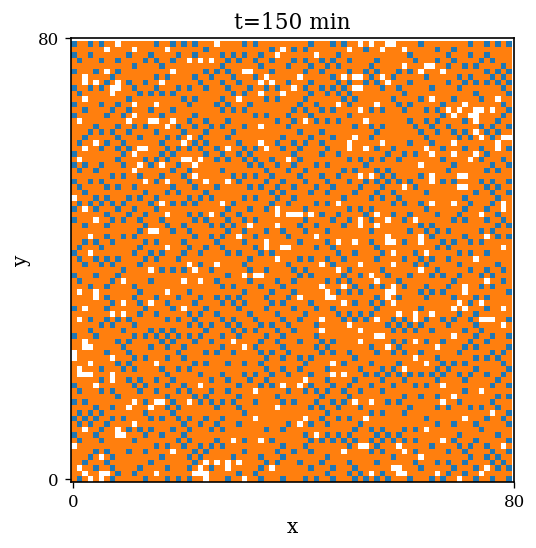
\includegraphics[width=\linewidth]{results/2d_5_snap.png}
        %\caption{Imagen 5}
    \end{subfigure}\hfill
    \begin{subfigure}[t]{0.25\textwidth}
        \centering
        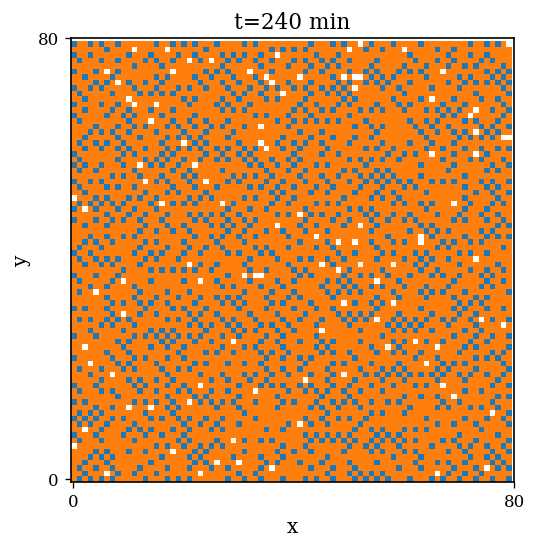
\includegraphics[width=\linewidth]{results/2d_6_snap.png}
        %\caption{Imagen 6}
    \end{subfigure}

    \caption{Snapshots en diferentes tiempos del crecimiento en el modelo 2D.}
    \label{fig:seis_imagenes_2x3}
\end{figure}\\


\begin{figure}[h!]
    \centering
    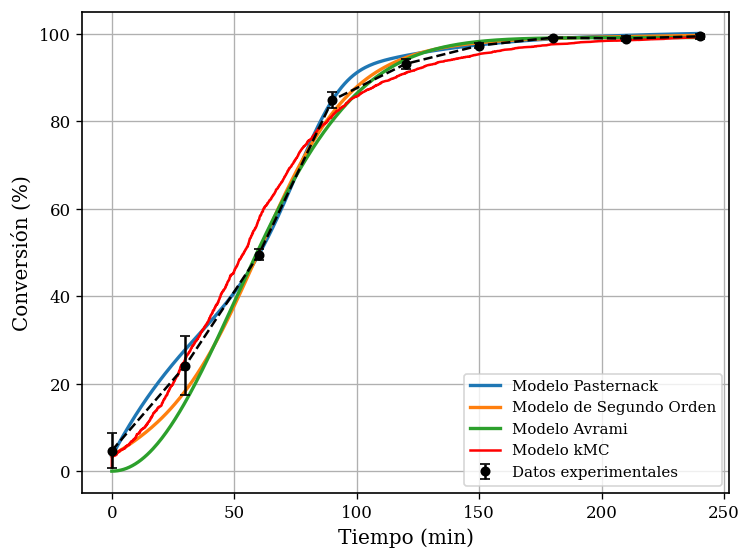
\includegraphics[width=0.5\linewidth]{results/2d_conv.png}
    \caption{Ajuste del modelo kMC 2D isotrópico y su comparación con los modelos cinéticos.}
    \label{fig:cinetica2d}
\end{figure}\\

\begin{table}[h!]
\centering
\caption{Comparativa de los parámetros de bondad de ajuste ($R^2$ y RMSE) entre los modelos analíticos y el modelo estocástico.}
\label{tab:ajuste_kmc_2d}
\begin{tabular}{lcc}
\toprule
\textbf{Modelo} & \textbf{$R^2$} & \textbf{RMSE} \\
\midrule
Pasternack     & 0.998 & 1.49 \\
Segundo Orden  & 0.995 & 2.28 \\
Avrami         & 0.989 & 3.60 \\
Modelo kMC 2D& 0.991 & 2.10 \\
\bottomrule
\end{tabular}
\begin{tablenotes}
\small
\end{tablenotes}
\label{table:kMC2d}
\end{table}\\

\newpage


\section{Resultados para el modelo 3D}

La ejecución de las simulaciones para el modelo 3D también se realizó con un tamaño de $80\times80$ para la red de sitios de adsorción. El intervalo de tiempo simulado fue de $[0, 240]$ minutos.\\

Asimismo, se obtuvo la cinética de crecimiento superficial (figura \ref{fig:cinetica3d}) que a su vez se compara con los ajustes de los tres modelos de cinética de crecimiento (tabla \ref{table:kMC3d}). Se observa, en este caso, una reproducción un poco más deficiente que el modelo 2D. Sin embargo, se considera una reproducción satisfactoria de los datos de cinética de crecimiento.

\begin{figure}[h!]
    \centering
    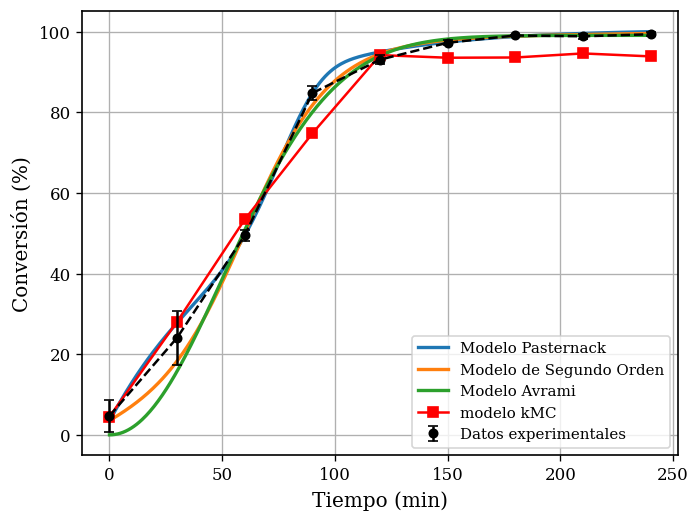
\includegraphics[width=0.6\linewidth]{results/3d_conv.png}
    \caption{Ajuste del modelo kMC 3D y su comparación con los modelos cinéticos.}
    \label{fig:cinetica3d}
\end{figure}

\begin{table}[h!]
\centering
\caption{Comparativa de los parámetros de bondad de ajuste ($R^2$ y RMSE) entre los modelos analíticos y el modelo estocástico.}
\label{tab:ajuste_kmc_3d}
\begin{tabular}{lcc}
\toprule
\textbf{Modelo} & \textbf{$R^2$} & \textbf{RMSE} \\
\midrule
Pasternack     & 0.998 & 1.49 \\
Segundo Orden  & 0.995 & 2.28 \\
Avrami         & 0.989 & 3.60 \\
modelo kMC 3D& 0.971 & 4.69 \\
\bottomrule
\end{tabular}
\begin{tablenotes}
\small
\end{tablenotes}
\label{table:kMC3d}
\end{table}

Por su parte, la morfología reproducida por el modelo 3D tiene dos vertientes. Por un lado, está la parte isotrópica, cuyos parámetros se calibraron mediante un ajuste de optimización Bayesiana. Para este caso, y mediante el uso de dicha herramienta, se obtuvieron los valores de $E_{pb}/k_BT = 1.27$, $\phi/k_BT = 1.48$, $\delta = 1.78$, $K_0^+ = 11.67$, $K_{inc}^+ = 0.507$. Por otro lado, para la vertiente anisotrópica, los parámetros se calibraron con una combinación de lo obtenido mediante optimización Bayesiana para $\phi/k_BT$, $\delta$, $K_0^+$ y $K_{inc}^+$; y los cálculos \textit{ab initio} de la sección \ref{sec:abini} para $E_{pb_x}$ y $E_{pb_y}$. Se utilizaron los valores de la dirección de enlace $\mu$-Propionato para $E_{pb_x}$ y la dirección de enlace $P-P$ para $E_{pb_y}$, cuyas magnitudes están descritas en la tabla \ref{table:MACE}. En las figuras \ref{fig:snaps_iso} y \ref{fig:snaps_aniso} se observan las morfologías de crecimiento superficial reproducidas por el modelo 3D, para valores $\sigma = 0.38$, $\sigma = 1.5$ y $\sigma = 2.7$ respectivamente.\\


\begin{figure}[h!]
    \centering
    
    \begin{subfigure}[t]{0.33\textwidth}
        \centering
        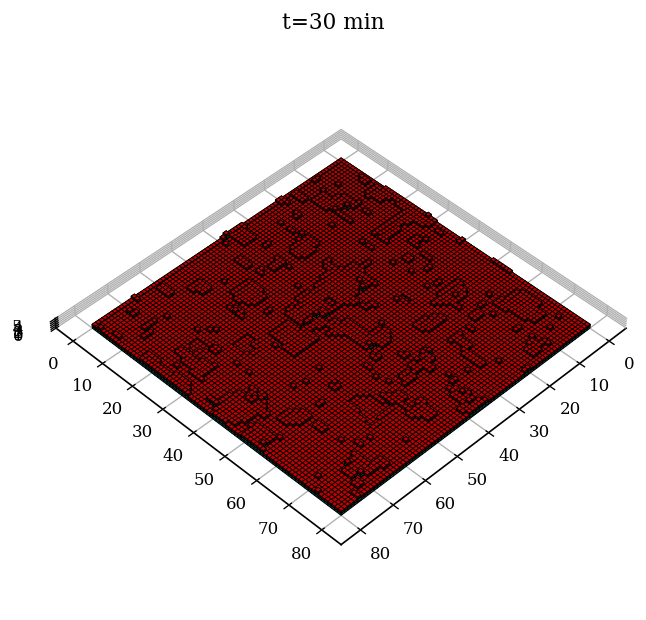
\includegraphics[width=\linewidth]{results/iso_c_1_1.png}
        %\caption{Imagen 1}
    \end{subfigure}\hfill
    \begin{subfigure}[t]{0.33\textwidth}
        \centering
        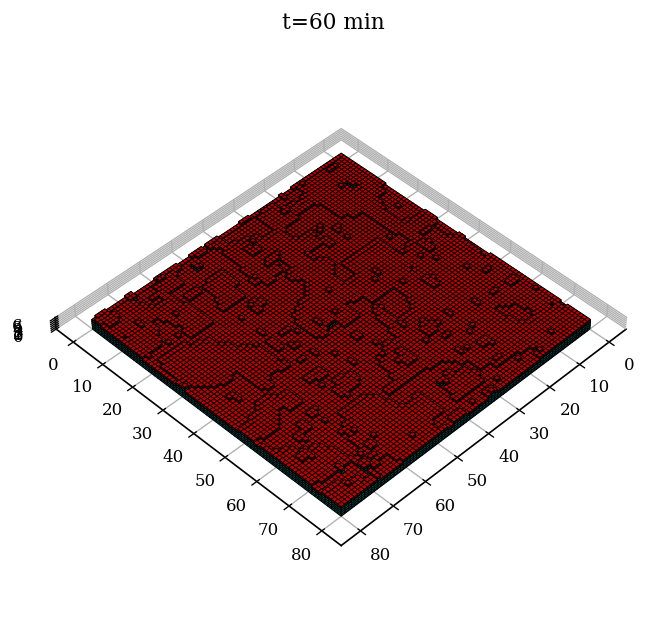
\includegraphics[width=\linewidth]{results/iso_c_2.png}
        %\caption{Imagen 2}
    \end{subfigure}\hfill
    \begin{subfigure}[t]{0.33\textwidth}
        \centering
        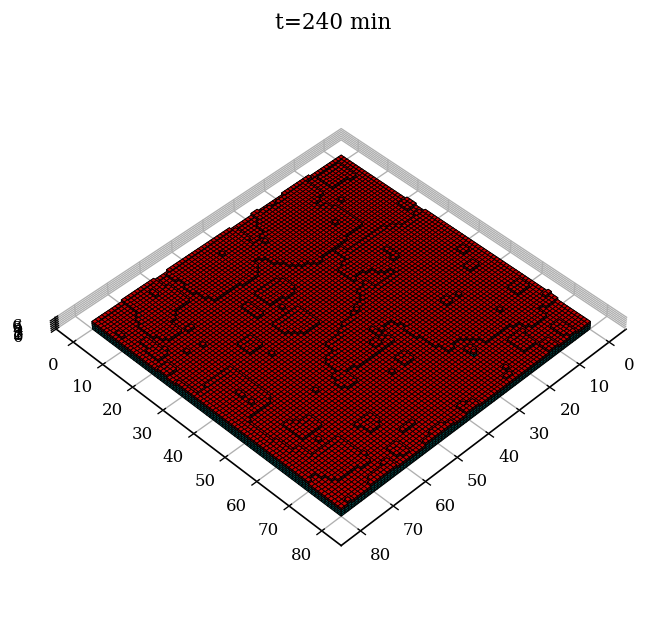
\includegraphics[width=\linewidth]{results/iso_c_3.png}
        %\caption{Imagen 3}
    \end{subfigure}

    \vspace{0.3cm}

    \begin{subfigure}[t]{0.33\textwidth}
        \centering
        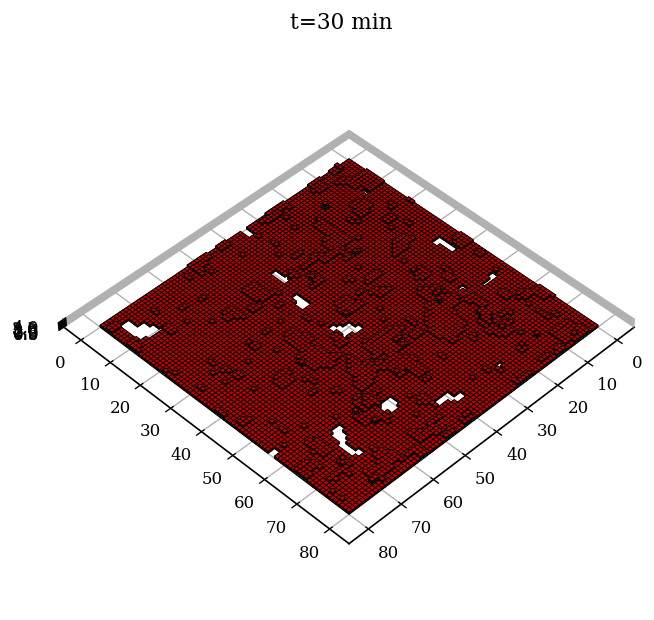
\includegraphics[width=\linewidth]{results/iso_d_1.png}
        %\caption{Imagen 4}
    \end{subfigure}\hfill
    \begin{subfigure}[t]{0.33\textwidth}
        \centering
        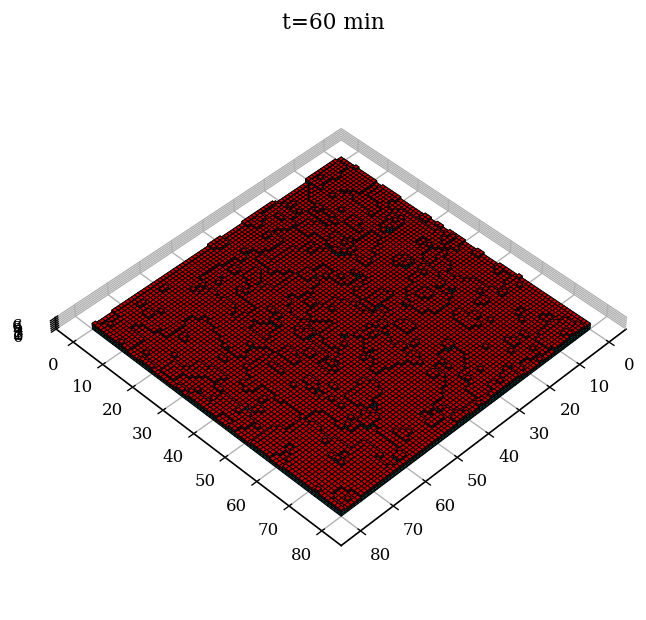
\includegraphics[width=\linewidth]{results/iso_d_2.png}
        %\caption{Imagen 5}
    \end{subfigure}\hfill
    \begin{subfigure}[t]{0.33\textwidth}
        \centering
        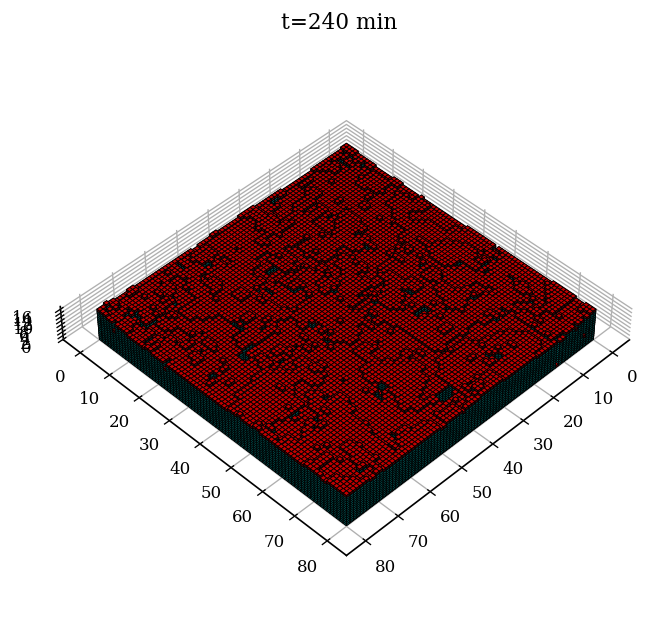
\includegraphics[width=\linewidth]{results/iso_d_3.png}
    \end{subfigure}

    \vspace{0.3cm}
    \begin{subfigure}[t]{0.33\textwidth}
        \centering
        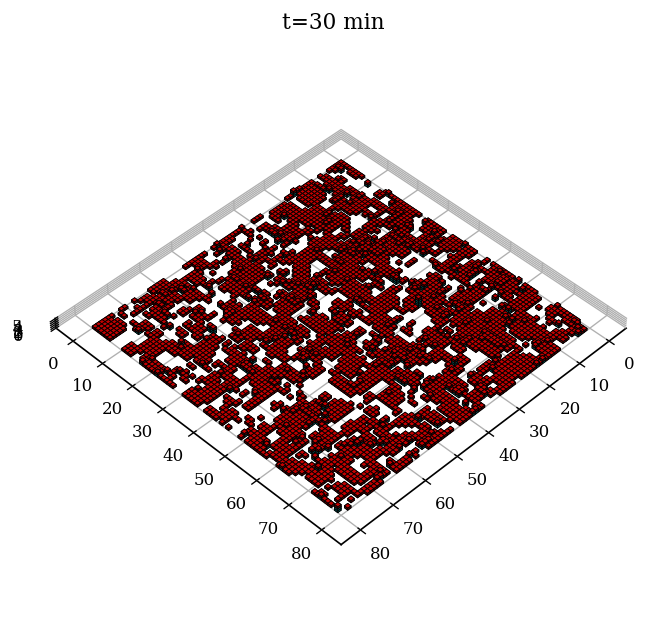
\includegraphics[width=\linewidth]{results/iso_e_1.png}
        %\caption{Imagen 4}
    \end{subfigure}\hfill
    \begin{subfigure}[t]{0.33\textwidth}
        \centering
        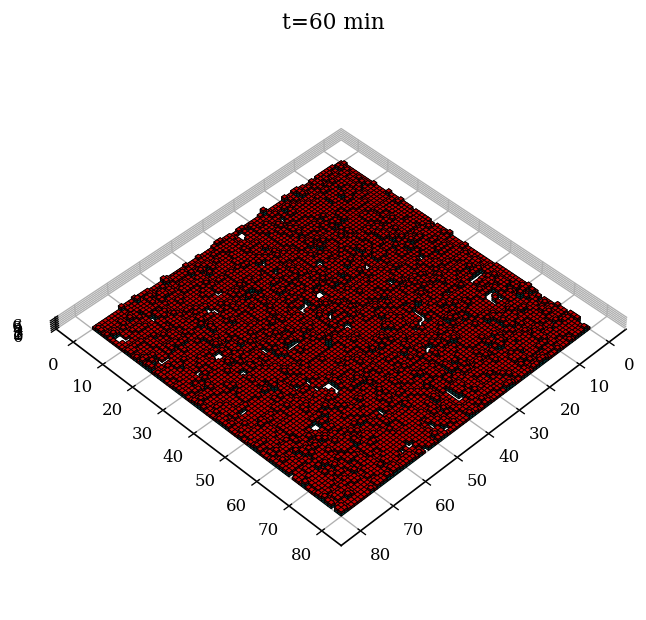
\includegraphics[width=\linewidth]{results/iso_e_2.png}
        %\caption{Imagen 5}
    \end{subfigure}\hfill
    \begin{subfigure}[t]{0.33\textwidth}
        \centering
        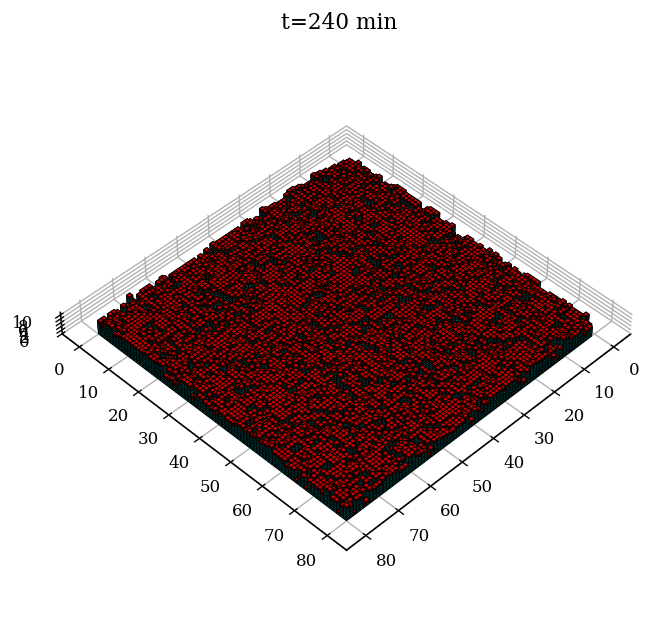
\includegraphics[width=\linewidth]{results/iso_e_3.png}
    \end{subfigure}

    \caption{Snapshots en diferentes tiempos del crecimiento en el modelo 3D isotrópico.}
    \label{fig:snaps_iso}
\end{figure}\\



\begin{figure}[h!]
    \centering
    
    \begin{subfigure}[t]{0.33\textwidth}
        \centering
        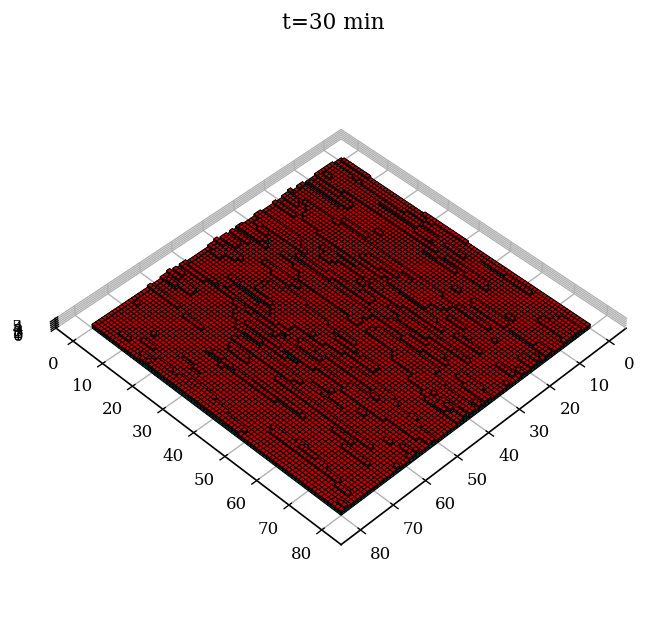
\includegraphics[width=\linewidth]{results/aniso_c_1.png}
        %\caption{Imagen 1}
    \end{subfigure}\hfill
    \begin{subfigure}[t]{0.33\textwidth}
        \centering
        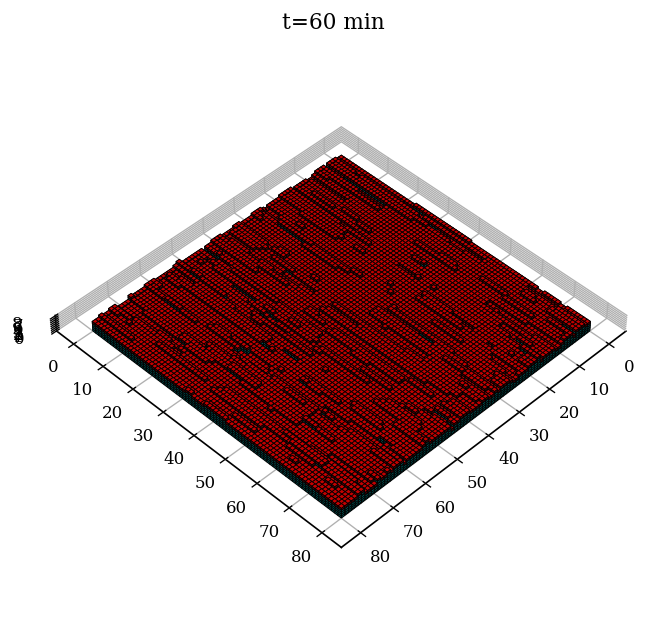
\includegraphics[width=\linewidth]{results/aniso_c_2.png}
        %\caption{Imagen 2}
    \end{subfigure}\hfill
    \begin{subfigure}[t]{0.33\textwidth}
        \centering
        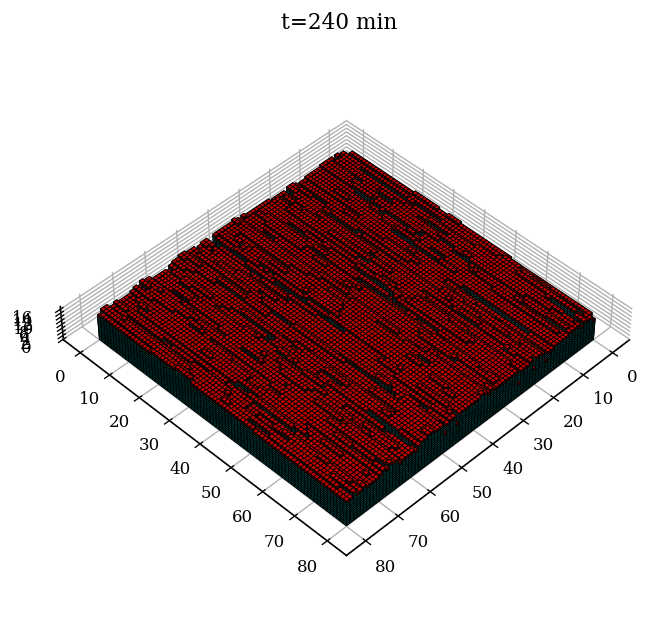
\includegraphics[width=\linewidth]{results/aniso_c_3.png}
        %\caption{Imagen 3}
    \end{subfigure}

    \vspace{0.3cm}

    \begin{subfigure}[t]{0.33\textwidth}
        \centering
        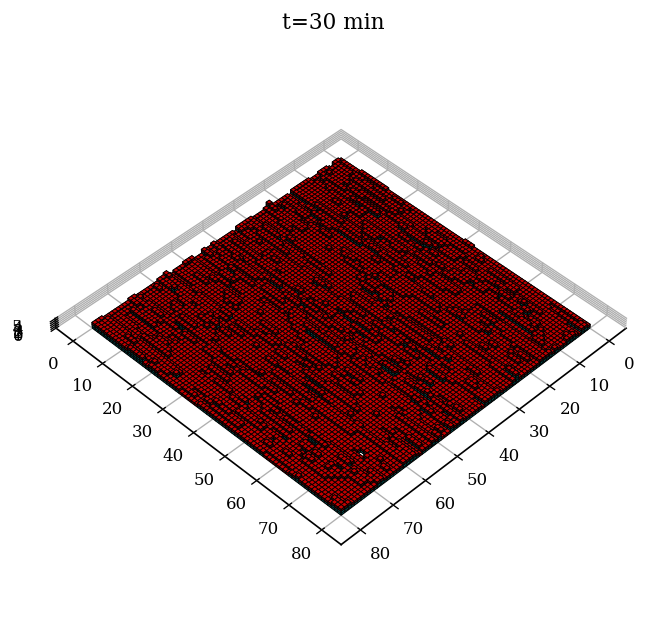
\includegraphics[width=\linewidth]{results/aniso_d_2.png}
        %\caption{Imagen 4}
    \end{subfigure}\hfill
    \begin{subfigure}[t]{0.33\textwidth}
        \centering
        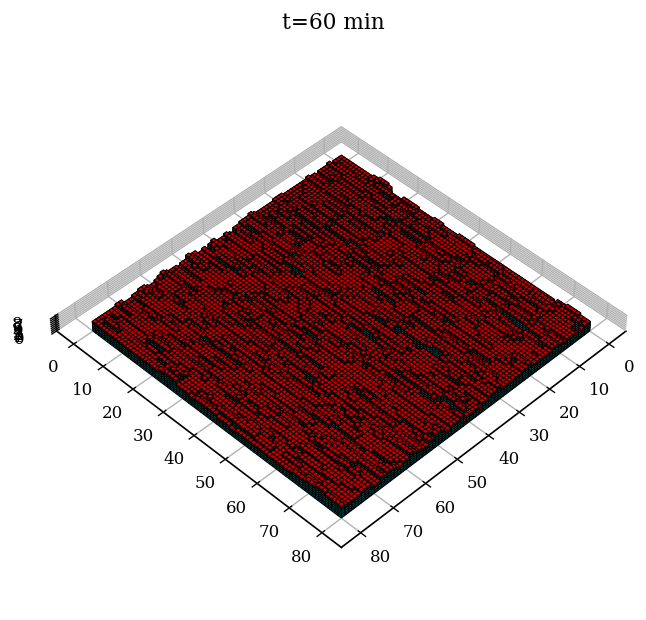
\includegraphics[width=\linewidth]{results/aniso_d_1.png}
        %\caption{Imagen 5}
    \end{subfigure}\hfill
    \begin{subfigure}[t]{0.33\textwidth}
        \centering
        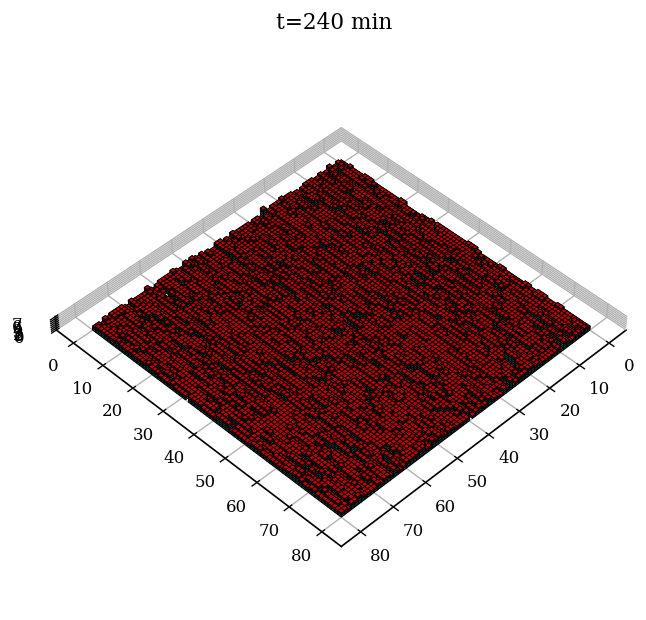
\includegraphics[width=\linewidth]{results/aniso_d_3.png}
    \end{subfigure}

    \vspace{0.3cm}
    \begin{subfigure}[t]{0.33\textwidth}
        \centering
        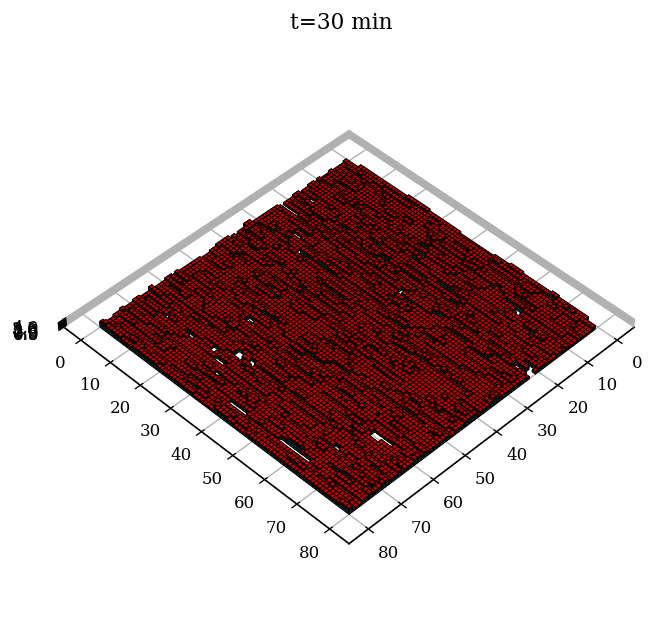
\includegraphics[width=\linewidth]{results/aniso_e_1.png}
        %\caption{Imagen 4}
    \end{subfigure}\hfill
    \begin{subfigure}[t]{0.33\textwidth}
        \centering
        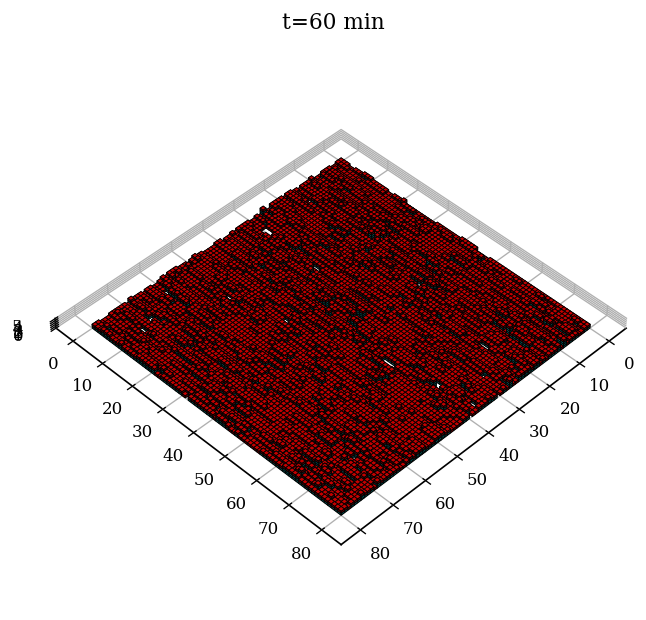
\includegraphics[width=\linewidth]{results/aniso_e_2.png}
        %\caption{Imagen 5}
    \end{subfigure}\hfill
    \begin{subfigure}[t]{0.33\textwidth}
        \centering
        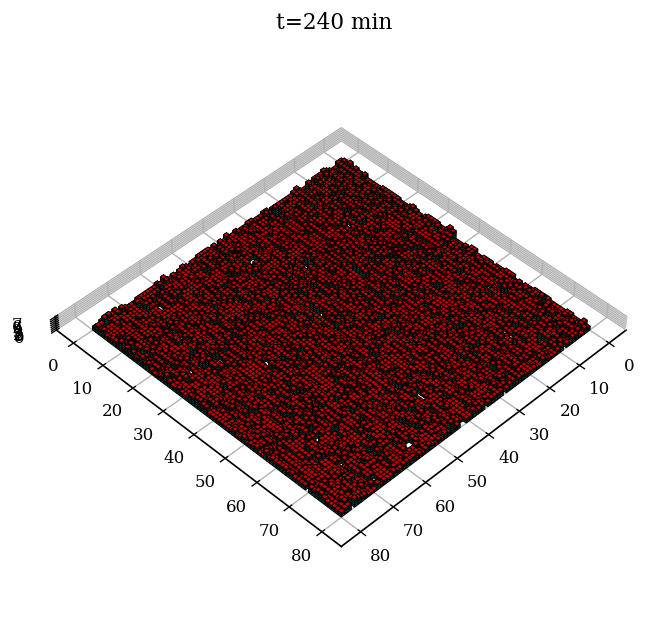
\includegraphics[width=\linewidth]{results/aniso_e_3.png}
    \end{subfigure}

    \caption{Snapshots en diferentes tiempos del crecimiento en el modelo 3D anisotrópico.}
    \label{fig:snaps_aniso}
\end{figure}\\

Los snapshots muestran la correspondencia directa entre el valor de sobresaturación (mediado por $\sigma$ en este trabajo) y el régimen de crecimiento, mostrando cualitativamente que, a medida que aumenta la sobresaturación, aumenta la rugosidad superficial de crecimiento, tanto para el crecimiento isotrópico como anisotrópico. Se nota que, cuando la sobresaturación es baja, hay convivencia entre islas más grandes con otras más pequeñas, bien diferenciadas. Pero, a medida que la sobresaturación crece, las islas van desapareciendo y el crecimiento es mucho más desordenado.\\

En un trabajo realizado por Olafson et al. en 2017 \cite{Olafson2017KineticRoughening}, obtienen imágenes de la evolución de la morfología superficial de la cara cristalográfica [100] de cristales de $\beta$-hematina durante su crecimiento a diferentes valores de sobresaturación, observada mediante microscopía de fuerza atómica (AFM por sus siglas en inglés) en modo de fase. Allí, ellos mismos señalan cómo a bajas sobresaturaciones el crecimiento ocurre mediante un mecanismo de nucleación bidimensional y propagación de escalones lo que produce superficies lisas y bien facetadas, y al incrementar la sobresaturación la densidad de núcleos sobre la superficie aumenta considerablemente y los escalones individuales dejan de distinguirse, dando lugar a una interfaz rugosa. Esta transición evidencia el cambio desde un crecimiento ordenado por capas hacia un crecimiento dominado por la nucleación simultánea de múltiples islas, fenómeno que constituye uno de los principales resultados experimentales reportados por Olafson et al. Estos resultados experimentales resultan interesantes para comparar con los resultados obtenidos mediante el modelo kMC, y se pueden observar en la figura \ref{fig:morfo_compa}.\\

\begin{figure}[h!]
    \centering
    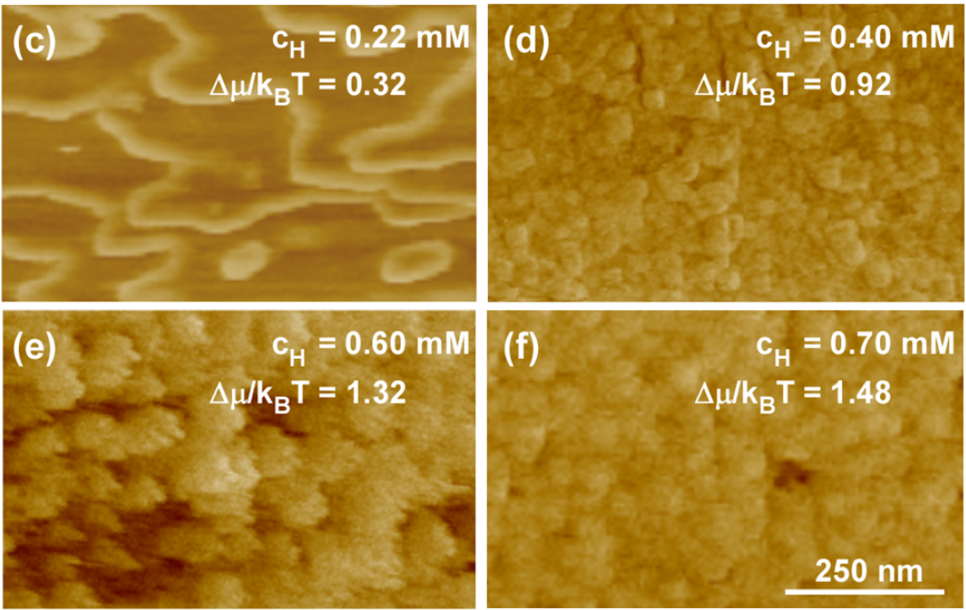
\includegraphics[width=0.8\linewidth]{figures/morfo_compara.png}
    \caption{Resultados experimentales del trabajo de Olafson et al. para la morfología superficial de crecimiento en función de la sobresaturación.}
    \label{fig:morfo_compa}
\end{figure}\\

Con el fin de garantizar la reproducibilidad computacional y transparencia de este trabajo, se dispus el código fuente de todas las implementaciones y simulaciones en un repositorio público de GitHub: \url{https://github.com/SebastGg99/MalariaProject}.


\chapter{Conclusiones y perspectivas}
A partir de los resultados obtenidos y las interpretaciones de los mismos, se puede llegar a las siguientes conclusiones:

\begin{itemize}
    \item El modelo 2D reproduce la cinética de crecimiento de cristales de HZ (BH) y se ajusta a los datos experimentales de manera satisfactoria.
    \item El modelo 2D no reproduce de manera cualitativa la morfología de crecimiento superficial de cristales de HZ (BH), esto debido a sus limitaciones geométricas.
    \item El modelo 2D sirve como un buen paso inicial para implementar el algoritmo BKL con la intención de crear un modelo kMC para simular el crecimiento de cristales de HZ. Sin embargo, se queda corto en cuanto a la morfología superficial. Por lo tanto, se hace notoria la necesidad de un modelo 3D.
    \item El modelo 3D, aunque de una manera un poco menos precisa, también reproduce la cinética de crecimiento de cristales de HZ (BH) y se ajusta a los datos experimentales satisfactoriamente.
    \item Tanto la variantes isotrópica como la anisotrópica del modelo 3D reproducen, al menos de forma cualitativa, la morfología de crecimiento superficial de cristales de HZ (BH), representando claramente las transiciones del régimen de crecimiento a mediad que cambia el valor de sobresaturación. Así, el modelo 3D representa una buena base para simular el crecimiento de cristales de HZ (BH) a partir del algoritmo BKL.
\end{itemize}\\

\subsubsection{Perspectivas}

Aunque el presente trabajo puede tener muchas y muy variadas perspectivas que abarcan muchos temas de estudio, voy a mencionar las más importantes a mi parecer:

\begin{itemize}
    \item Se pueden definir y calcular parámetros de orden para tener un registro más cuantitativo y menos cualitativo de la morfología de nucleación y crecimiento en el modelo 3D.
    \item El modelo 3D puede ser integrado y acelerado con Transformers de Series Temporales, como lo proponen Nagpal et al. en su trabajo.
    \item El modelo 3D puede ser extendido a uno mejorado que modele y simule el crecimiento de cristales de HZ (BH) en presencia de antimaláricos.
\end{itemize}

% ==========================================
% APÉNDICES Y BIBLIOGRAFÍA
% ==========================================

\newpage
%\begin{thebibliography}{99}
%\addcontentsline{toc}{chapter}{Bibliografía}

%\bibitem{ejemplo1}
%Autor. \textit{Título del libro}. Editorial, Año.

%\end{thebibliography}

\bibliographystyle{ieeetr} %unsrt, abbrv ieeetr
\bibliography{thesis_ref}
%\bibliography{ref_mace}

\end{document}